\documentclass[letterpaper,12pt,oneside]{book}
\usepackage{geometry}
\usepackage{amsmath}
\usepackage{amsfonts}
\usepackage{amssymb}
\usepackage{fancyhdr}
\usepackage{titlesec}
\usepackage{titletoc}
\usepackage{natbib}
%\usepackage{chapterbib}
\usepackage{graphicx}
\usepackage{etoolbox}
\usepackage{algorithm}
\usepackage{algpseudocode}
\usepackage{setspace}
\usepackage{tocloft}
\usepackage{caption}
\usepackage{footmisc}
\usepackage[nottoc,notlof,notlot]{tocbibind} % GET REFERENCES IN TOC

%% MAKE FOOTNOTES USE SYMBOLS INSTEAD OF NUMBER
%%%%%%%%%%%%%%%%%%%%%%%%%%%%%%%%%%%%%%%%%%%%%%%%%%%%%%%%%%%%%%%%%%%%%
\renewcommand{\thefootnote}{\fnsymbol{footnote}}

%% STOP GIVING SMALL FIGURES A FULL PAGE
%%%%%%%%%%%%%%%%%%%%%%%%%%%%%%%%%%%%%%%%%%%%%%%%%%%%%%%%%%%%%%%%%%%%%
\renewcommand{\floatpagefraction}{.6}

%% SET SMALLER FIGURE CAPTION FONT SIZE
%%%%%%%%%%%%%%%%%%%%%%%%%%%%%%%%%%%%%%%%%%%%%%%%%%%%%%%%%%%%%%%%%%%%%
\captionsetup[figure]{font=footnotesize,labelfont=footnotesize}
\captionsetup[table]{font=footnotesize,labelfont=footnotesize}

%% SET CHAPTERNONUM COMMAND
%%%%%%%%%%%%%%%%%%%%%%%%%%%%%%%%%%%%%%%%%%%%%%%%%%%%%%%%%%%%%%%%%%%%%
\newcommand{\chapternonum}[1]{\chapter*{#1}
                              \addcontentsline{toc}{chapter}{#1}}

%% SET NEWAPPENDIX COMMAND
%%%%%%%%%%%%%%%%%%%%%%%%%%%%%%%%%%%%%%%%%%%%%%%%%%%%%%%%%%%%%%%%%%%%%
\newlistof{appendices}{apc}{\listappendicesname}
\newcommand{\addcontentslines}[1]{\addcontentsline{apc}{appendices}{#1}
                                  \addcontentsline{toc}{section}{#1}}
\newcommand{\newappendix}[1]{\section*{#1}
                             \addcontentslines{#1}}

%% SET SPACING
%%%%%%%%%%%%%%%%%%%%%%%%%%%%%%%%%%%%%%%%%%%%%%%%%%%%%%%%%%%%%%%%%%%%%
%\doublespacing
%\onehalfspacing
\singlespacing

%% INCLUDE THE WORD "CHAPTER" IN TOC
%%%%%%%%%%%%%%%%%%%%%%%%%%%%%%%%%%%%%%%%%%%%%%%%%%%%%%%%%%%%%%%%%%%%%
\titlecontents
{chapter}% section type
[0.0in]% spacing
{\vspace*{0.2in}} % space above code
{\bfseries CHAPTER \thecontentslabel:\ } % numbered entry format
{\bfseries} % numberless entry format
{\bfseries\hfill\contentspage} % blank filler
[\vspace{0.0in}] % space after code
%{\titlerule*[0.77pc]{.}\contentspage} % dotted filler line

%% CUTOMIZE CHAPTER TITLES
%%%%%%%%%%%%%%%%%%%%%%%%%%%%%%%%%%%%%%%%%%%%%%%%%%%%%%%%%%%%%%%%%%%%%
\titleformat
{\chapter} % command
[display] % shape
{\centering\bfseries\large} % format
{CHAPTER \thechapter} % label
{0.2in} % sep between number and name
{} % before-code

%% CUTOMIZE SECTION TITLES
%%%%%%%%%%%%%%%%%%%%%%%%%%%%%%%%%%%%%%%%%%%%%%%%%%%%%%%%%%%%%%%%%%%%%
\titleformat
{\section}
[block] % Block puts the section number and name on the same line 
{\bfseries\large}
{\thesection}
{0.1in} % sep between number and name
{}

%% CUTOMIZE SUBSECTION TITLES
%%%%%%%%%%%%%%%%%%%%%%%%%%%%%%%%%%%%%%%%%%%%%%%%%%%%%%%%%%%%%%%%%%%%%
\titleformat
{\subsection}
[block] % Block puts the section number and name on the same line 
{\bfseries\normalsize} 
{\thesubsection}
{0.1in} % sep between number and name
{}

%% SET MARGINS
%%%%%%%%%%%%%%%%%%%%%%%%%%%%%%%%%%%%%%%%%%%%%%%%%%%%%%%%%%%%%%%%%%%%%
\geometry{top=1in,bottom=1in,left=1in,right=1in}

%% SET HEADER AND FOOTER
%%%%%%%%%%%%%%%%%%%%%%%%%%%%%%%%%%%%%%%%%%%%%%%%%%%%%%%%%%%%%%%%%%%%%
\pagestyle{fancy}
\fancyhf{}
\rhead{}
\lhead{}
\cfoot{\thepage}
\renewcommand{\headrulewidth}{0pt} % no horizontal line

%% SET LABLE AND STYLE FOR TOC, LIST OF FIGURES, AND LIST OF TABLES
%%%%%%%%%%%%%%%%%%%%%%%%%%%%%%%%%%%%%%%%%%%%%%%%%%%%%%%%%%%%%%%%%%%%%
\renewcommand*\contentsname{\centerline{\large{\textbf{TABLE OF CONTENTS}}}}
\renewcommand*\listfigurename{\centerline{\large{\textbf{LIST OF FIGURES}}}}
\renewcommand*\listtablename{\centerline{\large{\textbf{LIST OF TABLES}}}}
\newcommand*\listappendicesname{\centerline{\large{\textbf{LIST OF APPENDICES}}}}

%% CHANGE BIBLIOGRAPHY NAME TO REFERENCES
%%%%%%%%%%%%%%%%%%%%%%%%%%%%%%%%%%%%%%%%%%%%%%%%%%%%%%%%%%%%%%%%%%%%%
\renewcommand\bibname{REFERENCES}

%% CHANGE BIBLIOGRAPHY FROM A CHAPTER TO NUMBERED SECTION
%%%%%%%%%%%%%%%%%%%%%%%%%%%%%%%%%%%%%%%%%%%%%%%%%%%%%%%%%%%%%%%%%%%%%
%\renewcommand{\bibsection}{\section{\bibname}}

\begin{document}
%% FRONT MATTER
%%%%%%%%%%%%%%%%%%%%%%%%%%%%%%%%%%%%%%%%%%%%%%%%%%%%%%%%%%%%%%%%%%%%%
\frontmatter % sets roman numeral page numbering

%% TITLE PAGE
%%%%%%%%%%%%%%%%%%%%%%%%%%%%%%%%%%%%%%%%%%%%%%%%%%%%%%%%%%%%%%%%%%%%%
\thispagestyle{empty} % removes page numbering
\begin{singlespacing} % make just the title page single spaced
\begin{center}
\vspace*{1.5in}
\textbf{\large{Transient Ground Deformation in Tectonically Active
Regions and Implications for the Mechanical Behavior of the Crust and
Upper Mantle}}

\vspace*{0.2in}
by

\vspace*{0.2in}
Trever T. Hines 

\vspace*{1.0in}
A dissertation submitted in partial fulfillment

of the requirement for the degree of 

Doctor of Philosophy

(Earth and Environmental Sciences)

in the University of Michigan

2017
\end{center}
\vspace*{1.5in}
Doctoral Committee:

\vspace*{0.1in}
\hspace*{0.2in}
Associate Professor Eric Hetland, Chair

\hspace*{0.2in}
Associate Professor Jeremy Bassis

\hspace*{0.2in}
Professor Jeroen Ritsema

\hspace*{0.2in}
Professor John Boyd

\hspace*{0.2in}
Associate Professor Nathan Niemi

\end{singlespacing}
\newpage

%% IDENTIFIER
%%%%%%%%%%%%%%%%%%%%%%%%%%%%%%%%%%%%%%%%%%%%%%%%%%%%%%%%%%%%%%%%%%%%%
\thispagestyle{empty} % removes page numbering
\begin{center}
\vspace*{1.0in}
Trever T. Hines

hinest@umich.edu

ORCID iD: 9999-9999-9999-9999
\end{center}
\newpage

%% ACKNOWLEDGEMENTS
%%%%%%%%%%%%%%%%%%%%%%%%%%%%%%%%%%%%%%%%%%%%%%%%%%%%%%%%%%%%%%%%%%%%%
\chapternonum{ACKNOWLEDGEMENTS}

Blerg blargle blorg blerp 

\newpage

%% PREFACE
%%%%%%%%%%%%%%%%%%%%%%%%%%%%%%%%%%%%%%%%%%%%%%%%%%%%%%%%%%%%%%%%%%%%%
\chapternonum{PREFACE}

Blerg blargle blorg blerp 

\newpage

%% TABLE OF CONTENTS
%%%%%%%%%%%%%%%%%%%%%%%%%%%%%%%%%%%%%%%%%%%%%%%%%%%%%%%%%%%%%%%%%%%%%
\tableofcontents
\newpage
\listoffigures\addcontentsline{toc}{chapter}{LIST OF FIGURES}
\newpage
\listoftables\addcontentsline{toc}{chapter}{LIST OF TABLES}
\newpage
\listofappendices\addcontentsline{toc}{chapter}{LIST OF APPENDICES}
\newpage

%% ABSTRACT
%%%%%%%%%%%%%%%%%%%%%%%%%%%%%%%%%%%%%%%%%%%%%%%%%%%%%%%%%%%%%%%%%%%%%
\chapternonum{ABSTRACT}

%% MAIN MATTER
%%%%%%%%%%%%%%%%%%%%%%%%%%%%%%%%%%%%%%%%%%%%%%%%%%%%%%%%%%%%%%%%%%%%%
\mainmatter

\chapter{Bias in estimates of lithosphere viscosity from interseismic deformation}

\section{Abstract}
The estimation of uniform viscosities representing the lower crust and uppermost mantle from post- or interseismic deformation ({\it i.e.}, apparent viscosities) is inherently biased with respect to a depth-dependence of the viscosities within each layer. Estimates are biased toward a more viscous lower crust or a less viscous lithospheric mantle, depending on the relative geometric mean viscosities of the two layers. When there is a low viscosity shear zone beneath the fault, apparent viscosities are close to that of the shear zone immediately after the earthquake, although the apparent viscosities increase significantly during the later interseismic period.  Inferences made from interseismic deformation that the lower crust is more viscous than the upper mantle may be entirely consistent with depth-dependent viscosity profiles that have a significant increase in viscosity from the lowermost crust to the uppermost mantle.

\section{Introduction}
Numerous studies in tectonically active regions have sought estimates of the viscosities of the ductile lithosphere, including the lower crust and uppermost mantle \citep[{\it e.g.},][]{Hetland2003,Pollitz2003,Pollitz2005,Johnson2007,Hearn2009}. Here we consider estimates of the ductile lithosphere made by fitting predictions of surface deformation from mechanical models to geodetic measurements of interseismic deformation, including both post- and interseismic deformation.  Most studies of interseismic deformation concluded that the lower crust has a higher viscosity than the uppermost mantle \citep{Burgmann2008,Thatcher2008}. The majority of mechanical models used in these studies approximated the ductile lithosphere using two homogeneous viscoelastic layers representing the lower crust and uppermost mantle \citep[{\it e.g.},][]{Hetland2003,Pollitz2003,Hearn2009}. These simplistic layered models are commonly used because they are computationally cheap and because geodetic data are only capable of resolving a limited number of independent rheologic parameters \citep[{\it e.g.},][]{Riva2009,Pollitz2010}.  However, the simplifications made in the layered models may result in inferred viscosities that are not directly applicable to the real viscosity structure of the ductile lithosphere \citep{Riva2009}.
Temperature increases with depth and viscosity has a strong temperature dependence \citep[{\it e.g.},][]{Kohlstedt1995}.  The viscosity of the ductile lithosphere also has a stress-dependence \citep[{\it e.g.},][]{Kohlstedt1995}, although  the ductile lithosphere is often approximated as Maxwell viscoelastic in these models \citep[{\it e.g.},][]{Hetland2003,Johnson2007,Riva2009, Yamasaki2012a}.  This may be a reasonable approximation if stresses resulting from coseismic deformation are small compared to background stresses.  The Newtonian viscosity inferred in postseismic deformation studies may not be constant over time and could be interpretted as an effective viscosity of a power-law creep \citep[{\it e.g.},][]{Freed2006b}. Indeed, to describe geodetic observations, models of postseismic deformation in the months to years following an earthquake often require apparent viscosities up to several orders of magnitude smaller than those required in models of deformation later in the interseismic period \citep[{\it e.g.},][]{Pollitz2005,Johnson2007,Meade2013}. It is important to note that estimates of viscosities from the first few months following an earthquake may not be directly applicable to the steady viscosities of the lithosphere, as the immediate transient postseismic deformation is often considered to be due to postseismic fault creep, poroelastic rebound, or a transient rheology \citep[{\it e.g.},][]{Pollitz2003,Freed2006b,Hearn2009}. We save the investigation of models with non-linear, power-law creep and/or stress driven fault creep to a subsequent study, and here we only consider stress-linear viscoelasticity, allowing for a robust depth-dependence of viscosities.

We address the question of how inferences of single viscosities representing the entire lower crust and uppermost mantle are related to depth-dependent viscosities throughout the ductile lithosphere. We consider inferred viscosities made from rheologically idealized models of interseismic deformation to be apparent viscosities, and explore the biases incurred through using simplified models. For brevity, we use the term ``strength'' to refer to viscosity, or equivalently Maxwell relaxation time, $\tau_M$ ($\tau_M = \eta/\mu$, where $\eta$ is viscosity and $\mu$ is shear modulus), and thus we use ``strong'' or ``weak'' to refer to high or low viscosities, respectively. We show that estimates of the lithosphere's strength, based on simplified layered models, are almost always biased towards a stronger lower crust or a weaker upper mantle.

\section{Interseismic models}
We create synthetic surface deformation using 2D earthquake cycle models composed of an infinite length, vertical strike-slip fault in an elastic layer of thickness $D$ representing the upper crust, overlying a Maxwell viscoelastic substrate representing the ductile lithosphere (Figure 1). We impose uniform slip on the fault with repeat time $T$, until the surface deformation reaches a cycle invariant state ({\it i.e.}, the model is spun-up). The lower viscoelastic substrate is composed of a layer of thickness $D$, representing the lower crust, and a layer of thickness $8D$, representing the lithospheric mantle. We choose the thickness of the latter to be large enough such that the specific thickness does not affect the surface deformation.  Below $10D$, in the asthenosphere, we assume a homogeneous viscosity of $10^{19}$ Pa$\cdot$sec to the base of the model domain.  Models of infinite length, vertical strike-slip faults are anti-symmetric, and we only model one side of the fault. We use the finite element program GeoFEST \citep{Lyzenga2000} and take the model domain to be $120D$ wide by $100D$ deep. We impose an anti-symmetry boundary condition on the model edge containing the fault, a far-field velocity, $v_T$, on the opposite boundary, chosen so that there is no net strain accumulation in each earthquake cycle, and the top and bottom of the model are stress free (the bottom of the model domain is sufficiently deep that the bottom stress free boundary condition does not affect the surface deformation).  We consider only Maxwell viscoelasticity, but include depth-dependent viscosities within the lower crust and uppermost mantle. We assume that the shear modulus is uniform throughout the model and that viscosities vary smoothly, except possibly at $z = 2D$ ({\it i.e.}, the Moho) and at $z = 10D$ ({\it i.e.}, base of the lithosphere).  We non-dimensionalize the spatial dimensions by the fault locking depth, $D$, and time by $T$, and thus the non-dimensional Maxwell relaxation time is $\tau = \tau_M/T$. 

\begin{figure}\label{Fig1}
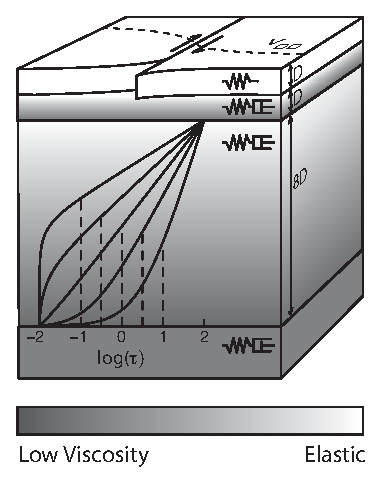
\includegraphics{ch1/figures/Figure1.eps}
\caption{Schematic of the earthquake cycle model: springs indicate elasticity and dashpots indicate Newtwonian viscosity. Example depth-dependent $\tau$ profiles are shown in the upper mantle, for the case when $\tau^{\min}_{UM} = 10^{-2}$, $\tau^{\max}_{UM} =10^{2}$, and $\bar{\tau}_{UM}$ indicated by vertical dotted lines.}
\end{figure}

\subsection{Depth-dependence of $\tau$}
Motivated by the fact that effective viscosity decreases exponentially with increasing temperature \citep[{\it e.g.},][]{Kohlstedt1995}, we take $\tau$ to decrease exponentially with depth. For generality, we do not assume any particular geotherm or composition of the ductile lithosphere, and instead specify that $\tau$ decreases in each layer as
\begin{equation}
\tau(z) = \alpha + \beta e^{-\gamma z},
\label{tau}
\end{equation}
where $z$ is depth within the layer, and $\alpha$, $\beta$, and $\gamma$ are parameters that vary for each layer.  The parameters in equation (\ref{tau}) depend on the maximum, $\tau_j^{\max}$, minimum, $\tau_j^{\min}$, and geometric mean, $\bar{\tau}_j$, relaxation times within layer $j$, where $j$ is ``LC'' or ``UM'' for the lower crust or mantle lithosphere, respectively.  We consider a wide range of viscosity profiles such that $10^{-1} \leq \tau_j^{\max} \leq 10^{2}$, $10^{-2} \leq \tau_j^{\min} \leq 10^{1}$, and $10^{-1} \leq \bar{\tau}_j \leq 10^{1}$, in increments of $10^{0.5}$.  With these ranges, we consider 5,625 depth-dependent lithosphere viscosity structures. The relaxation times are non-dimensionalized by $T$, so for a 100 year recurrence time, the shortest and longest Maxwell relaxation times we consider are 1 year and $10^{4}$ years, respectively (corresponding to viscosities of about $10^{18}$ Pa$\cdot$s and $10^{22}$ Pa$\cdot$s for $\mu \approx 30$ GPa).   Note that we consider profiles both in which the largest decrease of  $\tau$ is predominantly in the top or bottom of the layer (Figure 1), and we remark on the impact of this on our results below.

\section{Determination of apparent strength}
We define the apparent relaxation times (or equivalently the apparent viscosities) of the lower crust, $\hat{\tau}_{LC}$, and mantle lithosphere, $\hat{\tau}_{UM}$, as the relaxation times inferred from surface interseismic deformation using a model composed of constant viscosities in the two layers ({\it i.e.}, a layered model). In general, $\hat{\tau}_{LC}$ and $\hat{\tau}_{UM}$ have a temporal \citep{Riva2009} and spatial \citep{Yamasaki2012} dependence.  Both of which can be thought of as variables of interseismic surface deformation given a particular mechanical representation of the ductile lithosphere, but here we only consider the time dependence of inferred viscosities.  We denote the interseismic surface velocities in the models with depth-dependent $\tau$ as $v_{DD}$, and the velocities in a layered model as $v_{L}$.  We use a grid search to determine the $\hat{\tau}_j$ in a layered model that produced surface velocities that closest match the surface velocities in each of the depth-dependent models at 100 evenly spaced times throughout the interseismic period.  In the grid search, we search over $10^{-2} \leq \hat{\tau}_j \leq 10^2$, minimizing the root mean square error (RMSE) between $v_{DD}$ and $v_L$ at $0.5D$ increments of distance from the fault from $0.5D$ to $12D$\@.  We note that the upper limit of $\hat{\tau}_j$ searched over is a bit excessive because, for practical purposes, $v_{L}$ is insensitive to changes in relaxation time for $\tau \gtrsim 10^1$, as the layer is effectively elastic over interseismic periods \citep{Savage1978} (Auxiliary Figure 1).  Finally, we assume that the fault slip-rate and thickness of the lower crust and upper mantle are known.

About halfway through the interseismic period, surface deformation for almost all models we consider, both layered and depth-dependent, is indistinguishable from the deformation predicted by an elastic model with slip rate $v_T$ and locking depth $D$ \citep{Savage1973a} (Figure 2A). Because all models simultaneously predict surface interseismic velocities similar to the elastic model, $\hat{\tau}_j$ cannot be definitively resolved for a period during the middle of the earthquake cycle (Figure 3C). The exact times within the earthquake cycle in which the elastic model describes $v_{DD}$ as well as a layered model, depends on the specific $\tau$ profiles, but it is during the time period about $.4T$--$.5T$ for most of the models. 

\begin{figure}\label{Fig2}
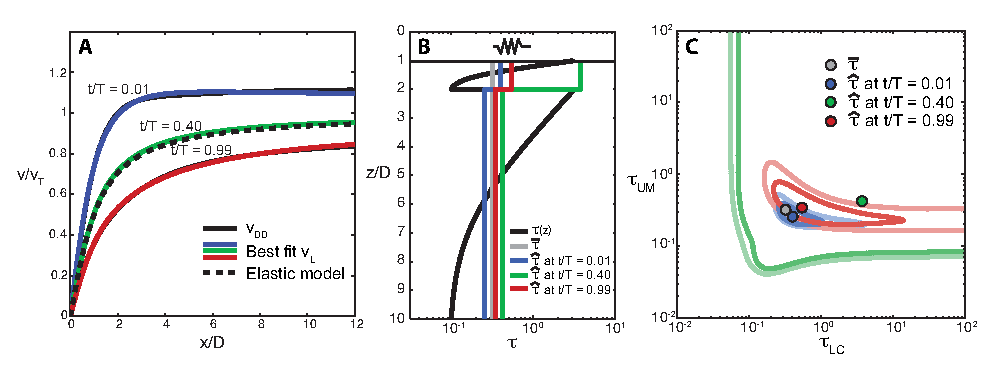
\includegraphics{ch1/figures/Figure2.eps}
\caption{A) Velocities for a depth-dependent model, $v_{DD}$ (black solid lines) and the best fitting velocities predicted by a layered model, $v_{L}$ (colored solid lines).  Black dashed line is the velocities predicted by an elastic earthquake model with the same $D$ and $v_{T}$.  B) $\tau$ profiles corresponding to $v_{DD}$ in (A) and $\hat{\tau}_j$ associated with the best fitting $v_{L}$ in (A).  C) $\bar{\tau}_j$ for the $\tau$ profile in (B) with $\hat{\tau}_j$ for each of the cases in (B). Solid lines indicate misfit contours in the grid-search estimation of $v_{L}$ in (A); contours shown are RMSE = 0.02 (dark lines) and 0.04 (faded lines), and color indicates the time.}
\end{figure}

\begin{figure}\label{Fig3}
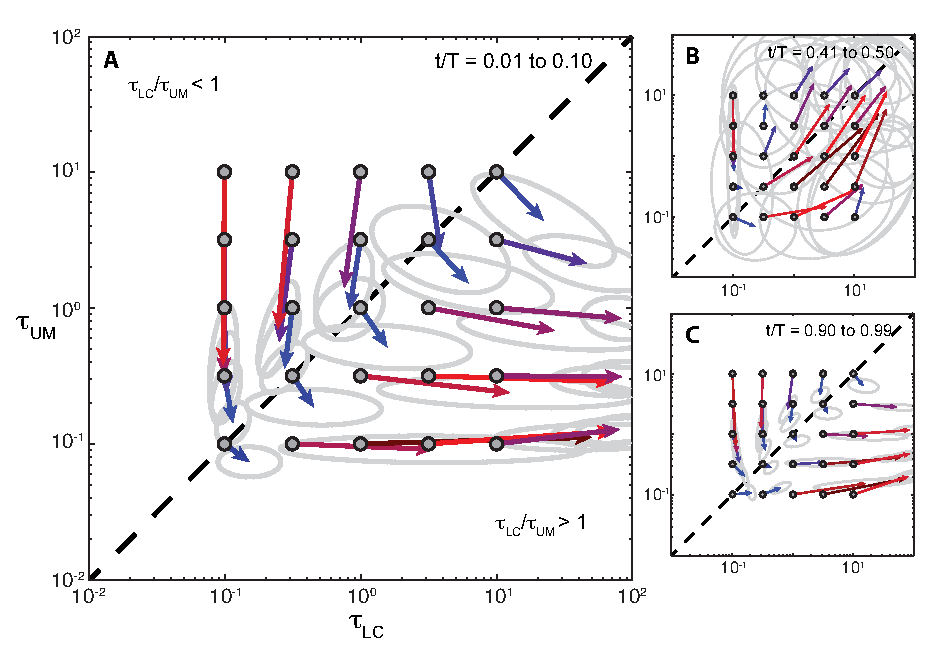
\includegraphics{ch1/figures/Figure3.eps}
\caption{$\bar{\tau}_j$ for all depth-dependent $\tau$ models considered (gray dots), along with the estimation Bias($\hat{\tau}_j$) (vectors) early (A), midway (B), and late (C) in the interseismic period.  Each vector points to the mean $\hat{\tau}_j$ estimated from depth-dependent models with the same $\bar{\tau}_j$, and the gray ovals indicate one standard deviation of $\hat{\tau}_j$.  The vector colors reflect the magnitude of the bias and help to distinguish overlapping vectors.}
\end{figure}

In general, the misfit between $v_{DD}$ and $v_{L}$ is largest early in the earthquake cycle for models with low $\bar{\tau}_{LC}$ and/or $\bar{\tau}_{UM}$ (Auxiliary Figure 2). The heightened misfit reflects the fact that there is more postseismic creep in the mid-crust and/or beneath the Moho in the layered models, resulting in differences in the wavelength of surface deformation compared to the depth-dependent models in which $\tau$ is larger in the mid-crust and/or beneath the Moho.  Misfit decreases to a minimum halfway into the earthquake cycle when deformation appears elastic.  The misfit increases again late in the earthquake cycle, although $v_{L}$ is a significantly better match to $v_{DD}$ compared to immediately after the earthquake.

We illustrate the determination of $\hat{\tau}_j$ using a model with a depth-dependent $\tau$ profile such that $\bar{\tau}_{LC} = \bar{\tau}_{UM} = 10^{-0.5}$, $\tau_{LC}^{\max} = \tau_{UM}^{\max} = 10^{0.5}$, and  $\tau_{LC}^{\min} = \tau_{UM}^{\min} = 10^{-1}$ (Figure 2). For this particular case, the misfit surfaces in the grid search shows clear minima and $\hat{\tau}_j$ is a fair approximation for $\bar{\tau}_j$ early and late in the interseismic period, although the lower crust relaxation time is slightly overestimated (Figure 2C). About halfway into the cycle, the layered model that best fits $v_{DD}$ dramatically overestimates the lower crust relaxation time (Figure 2B); however, there is a large range of $\hat{\tau}_j$ that would sufficiently match $v_{DD}$ (Figure 2C), since during this period the surface velocities for all models are very close to the velocities for the elastic model with identical fault slip rate and locking depth (Figure 2A). In this particular depth-dependent model, the velocities throughout the interseismic period are quite similar to those from elastic models, albeit with different slip rates and locking depths.

\section{Biases in apparent strength}
One might assume that the apparent $\tau$ estimated using a simple layered model, $\hat{\tau}_j$, reflects the geometric mean $\tau$ in those layers, $\bar{\tau}_j$. In general, $\hat{\tau}_j$ estimated from $v_{DD}$ at any time in one of the depth-dependent models may be significantly different than $\bar{\tau}_j$.  We consider the difference between the two values to be an error in the estimation of $\bar{\tau}_j$ and approximate the bias in the estimation throughout the interseismic period as
\begin{equation}
\mathrm{Bias}(\hat{\tau}_j; \bar{\tau}_j) = E[\hat{\tau}_j] - \bar{\tau}_j,
\label{bias}
\end{equation}
where $E[\hat{\tau}_j]$ is the geometric mean of $\hat{\tau}_j$ estimated from the collection of the depth-dependent models that all have the same $\bar{\tau}_j$. 

$\mathrm{Bias}(\hat{\tau}_j; \bar{\tau}_j)$ represents the bias in the estimated relaxation times for the lower crust and uppermost mantle with respect to the geometric mean relaxation time of the two layers.  In the wide range of models we considered, the bias depends on the contrast between the geometric mean relaxation times in the lower crust and upper mantle, $\bar{\tau}_{LC} /\bar{\tau}_{UM}$.  Early and late in the earthquake cycle there is a distinct bias towards an apparently weak upper mantle when $\bar{\tau}_{LC} / \bar{\tau}_{UM} < 1$ and a bias exaggerating the strength of the lower crust by up to a few orders of magnitude when $\bar{\tau}_{LC} / \bar{\tau}_{UM} > 1$ (Figure 3A,C).  About halfway through the interseismic period, the biases we calculate are not well constrained, but are generally towards a stronger lower crust and uppermost mantle (Figure 3B). These biases hold when we only consider $\tau$ profiles in which $\tau$ decays with depth faster than log-linearly (Auxiliary Figure 4), which indicates the biases are not sensitive to the specific decay of viscosity with depth provided that there is still some depth-dependence  within both layers.

When we consider models in which the lower crust is homogeneous, and include a depth-dependent $\tau$ only in the uppermost mantle, there is no clear bias when $\bar{\tau}_{LC} / \bar{\tau}_{UM} < 1$.  However, when  $\bar{\tau}_{LC} / \bar{\tau}_{UM} > 1$, there is a bias to a stronger lower crust and only a slight bias in the upper mantle strength (Auxiliary Figure 3A,C).  Conversely, when the uppermost mantle has a uniform relaxation time and $\tau$ is depth-dependent only in the lower crust, there is no bias when $\bar{\tau}_{LC} / \bar{\tau}_{UM} > 1$, but when $\bar{\tau}_{LC} / \bar{\tau}_{UM} < 1$ there is a bias towards a weaker upper mantle, while the lower crust relaxation time is accurately represented (Auxiliary Figure 3D,F). This may be counterintuitive, as one might think that if the lower crust or mantle was truly homogenous with respect to its relaxation time, then a simplified layered model should accurately capture that uniform relaxation time. In the case of both the lower crust and uppermost mantle being homogeneous, this would be true. However, if only one layer has a homogeneous relaxation time which is longer than the mean relaxation time in the depth-dependent layer, then strength estimates for that layer are biased.  This leads us to conclude that the biases are created by the depth-dependence of $\tau$ in the weaker of the two ductile lithospheric layers.

\section{Lower crustal shear zones}
It is likely that highly sheared rocks directly beneath a fault are considerably weaker than the surrounding lower crust \citep[{\it e.g.},][]{Montesi2003}, and lower crustal shear zones are well documented \citep[{\it e.g.},][]{Vauchez2003}. In all of the models that we present above, the largest $\tau$ in the lower crust is immediately beneath the fault.  These long relaxation times may suppress the relaxation of coseismic stresses in the lowermost crust, where the relaxation times are shorter, and thus may significantly influence our above conclusion that estimates of lower crustal strength are biased to stronger values than its geometric mean strength. To investigate the potential effect of a lower crustal shear zone on the biases in $\hat{\tau}_j$, we include a $D$ wide vertical shear zone extending through the lower crust beneath the fault.  We assume that the shear zone is Maxwell viscoelastic with a constant relaxation time of $\tau_{SZ} = 10^{-2}$, which is at least an order of magnitude faster than the surrounding lower crust. 

With a weak shear-zone, immediately following an earthquake the velocities are quite large, and as a result both the lower crust and uppermost mantle appear uniformly weaker than their geometric mean strength, with $\hat{\tau}_{LC}$ close to $\tau_{SZ}$ (Figure 4). These heightened postseismic velocities decay rapidly, although how $\hat{\tau}_{LC}$ or $\hat{\tau}_{UM}$ increases over time depends on $\bar{\tau}_{LC}/\bar{\tau}_{UM}$. If $\bar{\tau}_{LC}/\bar{\tau}_{UM} > 1$ then $\hat{\tau}_{LC}$ increases by orders of magnitude, exceeding $\bar{\tau}_{LC}$  (Figure 4B).  Otherwise, $\hat{\tau}_{UM}$ rapidly increases early in the cycle. For all models,  $\hat{\tau}_j$ evolves towards a more reasonable approximation of $\bar{\tau}_j$ late in the cycle  (Figure 4B). Additionally, the velocities are relatively steady throughout the later interseismic period compared to a model without a shear zone but with similar heightened postseismic velocities (Figure 4A).

\begin{figure}\label{Fig4}
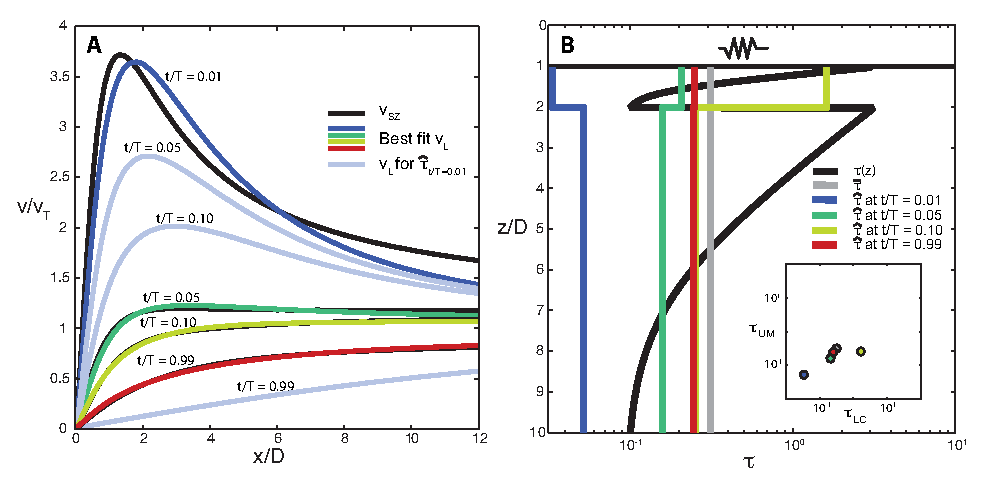
\includegraphics{ch1/figures/Figure4.eps}
\caption{A) Interseismic velocities, $v_{SZ}$, in a model with both a lower crustal shear zone and depth-dependent $\tau$ in the surrounding lithosphere (black lines) along with the best fit $v_{L}$ (colored lines).  Shown as light blue lines are the velocities in a layered model with the dark blue viscosity profile shown in (b), which are the apparent viscosities estimated from $v_{SZ}$ at $t/T = 0.01$.  B)  $\tau$ profile outside of the shear zone corresponding to $v_{SZ}$ (black line; $\tau$ = $10^{-2}$ within the shear zone), $\bar{\tau}$ outside the shear zone, and $\hat{\tau}_j$ associated with the best fitting $v_{L}$ in (A) (colored lines, color corresponds to time in cycle). Inset in (B) shows $\bar{\tau}_j$ and $\hat{\tau}_j$ (dot color corresponds to line colors in (A) and (B)).}
\end{figure}

\section{Discussion}
In the wide range of cases we consider, the biases in $\hat{\tau}_j$ inferred throughout the interseismic period almost always are such that $\hat{\tau}_{LC}/\hat{\tau}_{UM}$ is larger than $\bar{\tau}_{LC}/\bar{\tau}_{UM}$, except for midway through the interseismic period when all velocities are close to the elastic limit (Figure 3B).  Additionally, $\hat{\tau}_{LC}$ is often larger than $\tau^{\max}_{LC}$ and $\hat{\tau}_{UM}$ is often lower that $\tau^{\min}_{UM}$.  In models where $\bar{\tau}_{LC} \ne \bar{\tau}_{UM}$, inferences of $\hat{\tau}_{LC}/\hat{\tau}_{UM}>1$ ($<1$) correspond to models in which $\bar{\tau}_{LC}/\bar{\tau}_{UM}>1$ ($<1$). In other words, a lower crust that appears stronger than the mantle when approximated by uniform strength layers corresponds to models in which the geometric mean strength of the lower crust is also stronger than that in the mantle, and {\it vice versa}.  We note that several of the $\tau$ profiles with $\bar{\tau}_{LC} > \bar{\tau}_{UM}$ are characterized by significant portions of the lowermost crust having much lower viscosities than the uppermost mantle.

The biases we present in this paper can be viewed as relating $\hat{\tau}_j$ to $\bar{\tau}_j$.  However, the specific relationship between $\hat{\tau}_j$ and $\bar{\tau}_j$ depends not only on the details of how $\tau$ varies in the ductile lithosphere, but also on the time in the interseismic period. In the latter regard, it is also important to note that we have assumed periodic offsets on an infinite length fault, whereas real earthquakes are non-periodic and finite.  It is also important to note that we grouped all $\tau$ profiles according to the $\bar{\tau}_j$ in each layer irrespective of $\tau^{\max}_j$ and $\tau^{\min}_j$, and only considered how profiles with the same $\bar{\tau}_j$ relate to $\hat{\tau}_j$.  For these reasons, these biases cannot be used to back-out specific depth-dependent $\tau$ profiles, or even unique $\bar{\tau}_j$, consistent with $\hat{\tau}_j$ estimated from geodetic data using a simplified model of the lithosphere.  The coherency of the bias estimates suggest that it may be possible to develop probabilistic relationships between $\hat{\tau}_j$ and $\bar{\tau}_j$, assuming that the general time within the earthquake cycle the geodetic data are sampling is known.  For example, if $\hat{\tau}_{LC} \approx 10^{1}$ and $\hat{\tau}_{UM} \approx 10^{-1}$ were inferred from geodetic data late in a seismic cycle, then those estimates would be equivalent to depth-dependent $\tau$ profiles with $\bar{\tau}_{LC}$ around $10^{-0.5}$ to $10^{1}$ and $\bar{\tau}_{UM}$ on order of $10^{-1}$ (Figure 3C). Further exploration of the relationships between specific $\tau$ profiles and $\hat{\tau}_j$ would be required in order to establish whether inferences of apparent strength could be used to constrain the range of permissible $\tau$ profiles that are consistent with surface deformation at any one time.  It may also be possible to constrain depth-dependent $\tau$ profiles by considering how inferred viscosities vary as a function of distance from the fault \citep{Yamasaki2012}.

In the depth-dependent $\tau$ models we consider, the postseismic velocities are either only slightly above the elastic velocities or are large but decay over a relatively long portion of the interseismic period. Both of these cases are in contrast with many observations of heightened postseismic velocities decaying over on order of a decade following earthquakes \citep[{\it e.g.},][]{Ergintav2009}. Models including transient rheologies or power-law creep have been proposed to explain transient postseismic velocities \citep[{\it e.g.},][]{Pollitz2003,Freed2006b,Ryder2007}.  Adding a weak shear zone to a model with depth-dependent $\tau$ and only Maxwell viscoelasticity can also result in heightened postseismic velocities that rapidly decay over the postseismic period, while the surface velocities throughout the majority of the latter interseismic period are only slightly depressed compared to those in an elastic model with identical slip-rate and locking depth (Figure 4A).

\section{Conclusions}
  Assuming a uniform viscosity for the lower crust and uppermost mantle results in biased estimates of viscosity for those two layers if the viscosity is highly depth-dependent.  Estimates of viscosity tend to be biased either towards a weaker upper mantle or a stronger lower crust, depending on the relative viscosity of the two layers.  When there is a low viscosity lower crustal shear zone present, immediately after the earthquake the lower crust and uppermost mantle both appear weak, with apparent viscosities close to that of the shear zone, and then the apparent strength of the lower crust or upper mantle increases dramatically over the early interseismic period.  Using simplified models, inferences made from interseismic deformation that the lower crust is orders of magnitude more viscous than the upper mantle may be entirely consistent with depth-dependent viscosity profiles that have smaller contrasts between the geometric mean viscosities of lower crust and upper mantle and may be associated with a significant increase in viscosity across the Moho.

\section{Acknowledgments}
This research was funded by NSF grant EAR 1045372. We thank editor E. Calais, G. Houseman, and an anonymous reviewer.

\bibliographystyle{agu04}
\bibliography{refs}







\chapter{Rapid and simultaneous estimation of fault slip and heterogeneous lithospheric viscosity from postseismic deformation}

\section{Summary}
Postseismic deformation is commonly attributed to viscoelastic
relaxation and/or afterslip, although discerning between the two
driving mechanisms can be difficult.  A major complication in modeling
postseismic deformation is that forward models can be computationally
expensive, making it difficult to adequately search model space to
find the optimal fault slip distribution and lithospheric viscosity
structure that can explain observable postseismic deformation.  We
propose an inverse method which uses coseismic and early postseismic
deformation to rapidly and simultaneously estimate a fault slip
history and an arbitrarily discretized viscosity structure of the
lithosphere. Our method is based on an approximation which is
applicable to the early postseismic period and expresses surface
deformation resulting from viscoelastic relaxation as a linearized
function with respect to lithospheric fluidity.  We demonstrate this
approximation using two-dimensional earthquake models.  We validate
the approximation and our inverse method using two three-dimensional
synthetic tests. The success of our synthetic tests suggests that our
method is capable of distinguishing the mechanisms driving early
postseismic deformation and recovering an effective viscosity
structure of the lithosphere.

\section{Introduction}
Geodetic observations of surface deformation in the months to years
following an earthquake are often attributed to afterslip
\citep[e.g.][]{Marone1991}, viscoelastic relaxation in the lithosphere
\citep[e.g.][]{Nur1974}, and/or poroelastic relaxation
\citep[e.g.][]{Peltzer1998}.  If postseismic deformation can be
entirely described by afterslip, then one could easily constrain the
spatial distribution of slip on prescribed fault geometries with a
linear least squares inversion \citep[e.g.][]{Harris1987,Burgmann2002,Freed2007},
which could then provide insight into the frictional properties of
faults \citep[e.g.][]{Hsu2006,Barbot2009}.  However, postseismic deformation
following large ($M_w\geq7$) earthquakes is often attributed to
viscoelastic relaxation in the lithosphere
\citep[e.g.][]{Hetland2003,Pollitz2003,Pollitz2005} or a combination of both afterslip
and viscoelastic relaxation \citep[e.g.][]{Freed2006a,Hearn2009,Johnson2009,Rollins2015}.
In such cases, postseismic deformation can be used to also constrain
the viscous properties of the lithosphere, although this is a more
difficult task than constraining just a slip distribution.  Not only
do the competing deformation mechanism need to be discerned, finding
the viscosity distribution of the lithosphere from postseismic
deformation is a computationally expensive nonlinear inverse problem.
Typically, the estimation of viscosities is approached with a forward
modeling, grid search or Monte Carlo method.  These forward modeling
techniques require the number of unknown parameters being estimated to
be small, meaning that significant and potentially inappropriate
modeling assumptions must be made.  Namely, studies seeking to
estimate the viscosity structure of the lithosphere often assume for
computational tractability that the lithosphere is composed of two or
three homogeneously viscoelastic layers, which may not be appropriate
for describing a more realistic depth dependent viscosity structure
\citep{Riva2009,Hines2013}.

In this paper we propose a relatively fast method to invert coseismic
and postseismic deformation to simultaneously estimate a
time-dependent distribution of fault slip and an arbitrarily
discretized viscosity structure of the lithosphere.  Our method is
based on an approximation which linearizes the rate of early
postseismic deformation with respect to the viscosity of the
lithosphere.  We demonstrate the effectiveness and limitations of our
method through two synthetic tests.

\section{Approximation for postseismic deformation} 
We assume that the lithosphere can be approximated as a Maxwell
viscoelastic material on the timescales of postseismic deformation,
where shear stress, $\mathbf{\sigma}$, and strain,
$\mathbf{\varepsilon}$, are related by
\begin{equation}
  \frac{\partial\mathbf{\varepsilon}}{\partial t}=\frac{\mathbf{\sigma}}{2\eta} + 
                              \frac{1}{2\mu}\frac{\partial\mathbf{\sigma}}{\partial t}.
\end{equation}
We use $\eta$ and $\mu$ to represent viscosity and shear modulus,
respectively.  This constitutive relationship implies that a sudden
strain from an earthquake will instantaneously stress the lithosphere
elastically (assuming the lithosphere is undergoing quasi-static
deformation).  Viscoelastic creep will initiate immediately after the
earthquake, where the initial viscous strain rate in each parcel of
the lithosphere will be proportional to the fluidity ($1/\eta$) in
that parcel, and independent of the fluidity elsewhere because the
initial stresses are only controlled by the elastic properties of the
lithosphere.  Stresses from the earthquake will dissipate over time
through viscoelastic relaxation.  During the period in which stress
changes from viscoelastic relaxation are small compared to the initial
elastic stresses, each parcel will continue to creep at a rate that is
approximately proportional to its fluidity.  In this early postseismic
period, the surface deformation from creep in each parcel will have an
amplitude that is also proportional to the fluidity in that parcel and
independent of the fluidity elsewhere.  As we will show, the early
surface expression of creep in the entire lithosphere is therefore a
sum of the surface deformation from each parcel and is linear with
respect to lithospheric fluidity.  We demonstrate this property of
early postseismic surface deformation in this section using simple
infinite length, strike-slip earthquake models, where the lithosphere
is approximated as a layered half-space. In Section \ref{SynthTest} we
consider two finite fault models with an arbitrarily discretized
lithospheric viscosity structure, the first with only Maxwell
viscoelasticity and the second with Burgers viscoelasticity.

\subsection{Two-dimensional earthquake models}\label{2DModel}
The easiest way to demonstrate how postseismic deformation can be
linearized with respect to lithospheric viscosity is with a
two-dimensional earthquake model consisting of a long, vertical,
surface rupturing, strike-slip fault that is embedded in a
viscoelastic horizontal layer overlying a viscoelastic half-space.  We
make use of the Correspondence Principle of Viscoelasticity
\citep[e.g.][]{Flugge1975}, which states that the Laplace transform of
deformation in a viscoelastic body has the same form as the Laplace
transform of deformation in a elastic body with the same geometry and
subjected to the same boundary conditions. The solution for
displacements following an earthquake in a viscoelastic lithosphere
can then be readily found provided that the corresponding elastic
solution is known \citep[e.g.][]{Nur1974,Savage1978,Hetland2005}.  One only
needs to replace the shear modulus in the Laplace transform of the
elastic solution with the effective viscoelastic shear modulus and
then compute the inverse Laplace transform.

\subsubsection{Two layered model}\label{2D2LModel}
From the solution of \citet{Rybicki1971}, surface displacements,
$u_{e}(x,t)$, resulting from slip on a fault in an elastic surface
layer overlying a semi-infinite elastic substrate are
\begin{equation}\label{TwoLayerElastic}
  u_{e}(x,t) = b(t)\left(\frac{1}{2} W(0) + 
    \sum_{n=1}^\infty \Gamma^nW(n)\right),
\end{equation}
where
\begin{equation}
  W(n) = \frac{1}{\pi}\left(\tan^{-1}\left(\frac{2nH + D}{x}\right) 
    - \tan^{-1}\left(\frac{2nH - D}{x}\right)\right)
\end{equation}
and
\begin{equation}
  \Gamma = \frac{\mu_1 - \mu_2}{\mu_1 + \mu_2}.
\end{equation}
In the above equation, $b(t)$ describes cumulative slip on the fault
through time and can describe coseismic slip and/or afterslip. $D$ is
the locking depth of the fault, $H$ is the thickness of the upper
layer, and $\mu_1$ and $\mu_2$ are the shear moduli in the upper
layer and lower substrate, respectively.  The Laplace transform of
eq. (\ref{TwoLayerElastic}) is
\begin{equation}\label{TwoLayerElasticLaplace}
 \hat{u}_e(x,s) = \hat{b}(s)\left(\frac{1}{2} W(0) +\sum_{n=1}^\infty\Gamma^nW(n)\right).
\end{equation}
We replace $\mu_1$ and $\mu_2$ in eq. (\ref{TwoLayerElasticLaplace})
with the equivalent shear moduli for Maxwell materials in the Laplace
domain, $\hat{\mu}_1$ and $\hat{\mu}_2$, to get the Laplace
transform of surface displacements in the two-layered, viscoelastic
half-space,
\begin{equation}\label{TwoLayerViscousLaplace}
 \hat{u}_v(x,s) = \hat{b}(s)\left(\frac{1}{2}W(0) +\sum_{n=1}^\infty\hat{\Gamma}^nW(n)\right),
\end{equation}
where
\begin{equation}
  \hat{\Gamma} = \frac{\hat{\mu_1} - \hat{\mu_2}}{\hat{\mu_1} + \hat{\mu_2}}
\end{equation}
and
\begin{equation}
  \hat{\mu_i} = \frac{s}{\frac{s}{\mu_i} + \frac{1}{\eta_i}}.
\end{equation}
To find the surface displacements in the time domain one must find the
inverse Laplace transform of eq. (\ref{TwoLayerViscousLaplace}), which
is typically done using the method of residues. However, we are
interested in characterizing the behavior of only the early
postseismic deformation and it serves us better to instead perform the
inverse Laplace transform with an extension of the initial value
theorem (Appendix A). We assume for simplicity that the shear modulus
for the viscoelastic lithosphere is homogeneous (i.e. $\mu_1 = \mu_2$)
and demonstrate in a supplementary IPython notebook that our
conclusions still hold when $\mu_1 \neq \mu_2$.  The surface
displacements in the time domain are
\begin{equation}
 u_v(x,t) = b(t)\frac{1}{2}W(0) + 
            b(t)\ast\mathcal{L}^{-1}\left[\sum_{n=1}^\infty\hat{\Gamma}^{n}W(n)\right],
\end{equation}
where we use $*$ to denote a convolution with respect to time.
Evaluating the above inverse Laplace transform using the method
described in Appendix A, we find
\begin{align}\label{TwoLayerViscous}
  u_v(x,t) = &b(t)\frac{1}{2}W(0) +\nonumber\\
             &b(t)\ast\left(\frac{\mu}{2\eta_2}W(1) - \frac{\mu}{2\eta_1}W(1)\right) +\nonumber\\
             &b(t)\ast\left(\left(\frac{\mu^2t}{4\eta_2^2} -
                  \frac{\mu^2t}{4\eta_1\eta_2}\right) \left(W(1) - W(2)\right) +
                  \left(\frac{\mu^2t}{4\eta_1\eta_2} - \frac{\mu^2t}{4\eta_1^2}\right)
                  \left(W(1) + W(2)\right)\right) + \nonumber\\ 
             &\dots.
\end{align}
The first term in eq. (\ref{TwoLayerViscous}) is the elastic response
to slip on the fault.  The remaining terms describe the surface
displacement due to viscoelastic relaxation.  We refer to the first of
these remaining terms as the initial viscoelastic response, which
describes surface deformation resulting from viscoelastic creep during
the period in which the stresses from fault slip are unaltered by
viscoelastic relaxation.  The initial viscoelastic response is linear
with respect to the fluidity in each of the two layers.

If the time since the rupture is sufficiently small compared to the
relaxation times of each layer, $\tau_i=\eta_i/\mu$, (i.e. the third
and following terms in eq. (\ref{TwoLayerViscous}) are small) and the
timescale of slip described by $b(t)$ is also short compared to the
relaxation times in the half-space, then we can truncate the series and
approximate early surface deformation using only the elastic response
and the initial viscoelastic response,
\begin{equation}\label{TwoLayerViscousApprox}
 u_v(x,t) \approx b(t)\frac{1}{2}W(0) + 
          \int_0^t b(\theta)\left(\frac{\mu}{2\eta_2}W(1) - 
                  \frac{\mu}{2\eta_1}W(1)\right)d\theta.
\end{equation} 
An approximation similar to eq. (\ref{TwoLayerViscousApprox}) was
demonstrated by \citet{Segall2010} for an elastic layer over a Maxwell
viscoelastic substrate. 

\begin{figure}
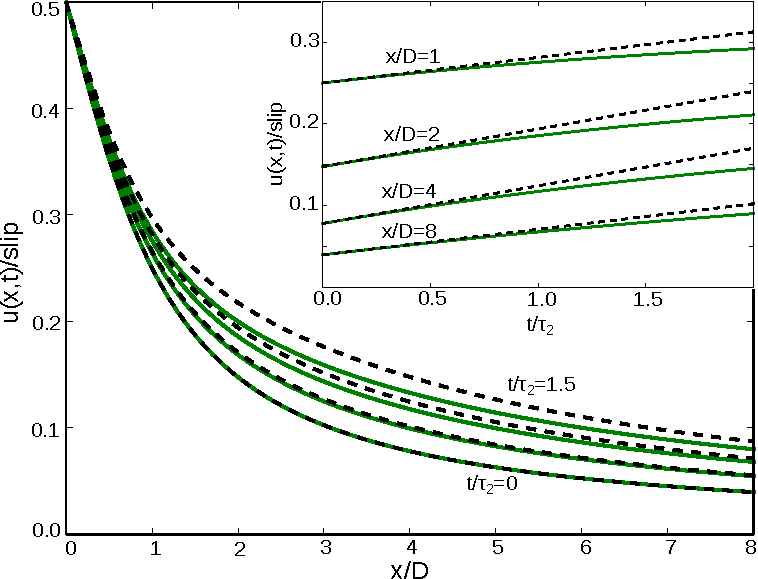
\includegraphics{ch2/figures/Fig1.pdf}
\caption{Surface displacements predicted by eq.
(\ref{TwoLayerViscous}) truncated after ten terms (green) and the
approximation given by eq. (\ref{TwoLayerViscousApprox}) (dotted
black).  Times are normalized by the lowest relaxation time in the
lithosphere, $\tau_2$, and distances are normalized by the fault
locking depth, $D$.  Displacements are shown as a function of distance
from the fault at times $t/\tau_2 = 0.0,0.5,1.0$ and $1.5$. The inset
figure shows displacement time series at locations $x/D = 1, 2, 4$ and
$8$.}
\label{figure1}
\end{figure} 

Fig. 1 shows the series solution from eq. (\ref{TwoLayerViscous})
truncated after sufficiently many terms along with the approximation
given by eq. (\ref{TwoLayerViscousApprox}). In this comparison, we use
$H=15$ km, $D=10$ km and a shear modulus of 32 GPa throughout the
lithosphere.  The upper layer is given a viscosity of $10^{20}$ Pa s
($\tau\approx 100$ years) and the substrate is given a viscosity of
$10^{19}$ Pa s ($\tau\approx 10$ years).  We let $b(t)$ describe a
unit of instantaneous slip at $t=0$.  In the series solution, the
rate of surface deformation decreases over time as stresses in the
half-space decay through viscoelastic relaxation.  Because $b(t)$ is a
constant after $t=0$, the initial viscoelastic response in
eq. (\ref{TwoLayerViscousApprox}) describes a constant rate of surface
deformation and so eq. (\ref{TwoLayerViscousApprox}) is a good
approximation for as long as the rate of deformation predicted by
eq. (\ref{TwoLayerViscous}) is also approximately constant. We find
the that the approximation is indistinguishable from the series
solution for at least as long as half the lowest of the two relaxation
times, regardless of our choice of model parameters.  The
approximation breaks down faster than what is show in Fig. 1 when
the upper layer is more fluid than the substrate or when we decrease the
depth of the material interface (i.e. when the more fluid material is
closer to the fault).  We also note that the approximation has more
longevity for locations further away from the fault, where it starts
to break down at about the minimum relaxation time in the lithosphere.

\subsubsection{Three layered and continuous depth dependent models}\label{2d3LModel}
We follow the same procedure as above to find the surface
deformation resulting from slip on a strike-slip fault in a three
layered viscoelastic half-space.  Starting from the layered elastic
solution from \citet{Chinnery1972}, we evaluate the solution for the
viscoelastic problem in our supplementary IPython notebook.  We find
the initial viscoelastic response to a unit of slip to be
\begin{equation}\label{ThreeLayerViscousResponse}
\frac{\partial}{\partial t}u(x,t)\big|_{t=0} = \frac{\mu}{2\eta_3}W(1,1)
                                      +\frac{\mu}{2\eta_2}(W(0,1) - W(1,1))
                                      -\frac{\mu}{2\eta_1}W(0,1),
\end{equation}
where
\begin{equation}
  W(n,m) = \frac{1}{\pi}\left(\tan^{-1}\left(\frac{2nH_2 + 2mH_1 + D}{x}\right) - 
                              \tan^{-1}\left(\frac{2nH_2 + 2mH_1 - D}{x}\right)\right),
\end{equation}
$\eta_1$, $\eta_2$, and $\eta_3$ are the viscosities of the top,
middle, and bottom layers, respectively, and $H_1$ and $H_2$ are the
thicknesses of the top and middle layers, respectively.  We see that
eq. (\ref{ThreeLayerViscousResponse}) is once again linear with
respect to the fluidity in each of the three layers.  We can
approximate early postseismic deformation resulting from slip
described by $b(t)$ as
\begin{equation}\label{ThreeLayerViscousApprox}
u(x,t) \approx b(t)\frac{1}{2} W(0,0) + 
         \int_0^tb(\theta)\left(\frac{\mu}{2\eta_3}W(1,1)
                               +\frac{\mu}{2\eta_2}(W(0,1) - W(1,1))
                               -\frac{\mu}{2\eta_1}W(0,1)\right)d\theta.
\end{equation}
We can see that eq. (\ref{ThreeLayerViscousApprox}) reduces to eq.
(\ref{TwoLayerViscousApprox}) when $\eta_3 = \eta_2$.

At this point we posit that a similar approximation can be made for an
arbitrarily layered lithosphere. In Appendix B we use
eq. (\ref{ThreeLayerViscousResponse}) to find an initial viscoelastic
response kernel.  We then integrate that kernel over the depth of the
lithosphere to find the initial viscoelastic response for an arbitrary
depth dependent viscosity structure.  If the lithosphere is elastic
above the fault depth, $D$, and described by $\eta(z)$ below $D$ then
early postseismic deformation can be approximated as
\begin{equation}\label{ContinuousViscousApprox}
u(x,t) \approx \frac{b(t)}{\pi}\tan^{-1}(\frac{D}{x}) + 
               \int_o^t\int_D^\infty \frac{\mu b(\theta)}{2\pi\eta(z)}
                                    \left(\frac{2x}{x^2 + \left(D + 2z\right)^2} - 
                                    \frac{2x}{x^2 + \left(2z - D\right)^2}\right)
                                    dz d\theta.
\end{equation}
Although the above equation is capable of describing surface
deformation for an arbitrary depth dependent viscosity structure, it
falls short of being useful as the forward solution in an inverse
problem aimed at estimating lithospheric viscosity.  This shortcoming
is because the above equation makes the nonphysical assumption that the
fault is infinitely long, in addition to the restriction of only being
applicable to a vertical strike-slip fault.  The assumption of
infinite length would introduce first order errors, which would likely
wash out the second order effect of viscosity. However,
eq. (\ref{ContinuousViscousApprox}) is useful for making estimates of
the depth sensitivity of postseismic deformation.

\subsection{Three-dimensional earthquake models}\label{3DModel}
Motivated by our above results, we make the assertion that the initial
viscoelastic response to an instantaneous unit dislocation in a
three-dimensional Maxwell viscoelastic medium, which has been
arbitrarily discretized into $N$ regions, will have the form
\begin{equation}\label{PostseismicInitialVelocity}
  \frac{\partial}{\partial t}\vec{u}(\vec{x},t)\big|_{t=0} = \sum_j^N\frac{1}{\eta_j}G_j(\vec{x}).
\end{equation}
We denote $\vec{u}$ and $\vec{x}$ as vectors to emphasize that
eq. (\ref{PostseismicInitialVelocity}) is generalized to
three-dimensional problems.  We use $G_j(\vec{x})$ to represent the
initial rate of surface deformation at position $\vec{x}$ resulting
from viscoelastic creep in region $j$ with unit fluidity, where
fluidity is zero (i.e. elastic) in all other regions.  In this sense,
$G_j(\vec{x})$ can be thought of as a Green's function for the initial
viscoelastic response, and thus we refer to $G_j(\vec{x})$ as the initial
viscoelastic Green's functions.  We verify
eq. (\ref{PostseismicInitialVelocity}) numerically in Section \ref{Validation} and
save a theoretical justification for a later paper.

Using eq. (\ref{PostseismicInitialVelocity}), we can approximate
early surface deformation in a form that is consistent with
eqs. (\ref{TwoLayerViscousApprox}) and
(\ref{ThreeLayerViscousApprox}):
\begin{equation}\label{intermediate}
\vec{u}(\vec{x},t) \approx b(t)F(\vec{x}) + \sum_j^N\int_0^t
\frac{b(\theta)}{\eta_j}G_j(\vec{x}) d\theta,
\end{equation}
where $F(\vec{x})$ is the elastic Green's function, which describes the
elastic deformation resulting from a dislocation.  We further
generalize the approximation of surface deformation in
eq. (\ref{intermediate}) to allow for an arbitrary spatial
distribution of slip by using linear superposition.  If the elastic
deformation in a viscoelastic lithosphere can be described in terms of
$M$ elastic dislocation sources, then early surface deformation
resulting from both elastic dislocations and viscous creep can be
approximated as 
\begin{equation}\label{Postseismic_Approximation}
\vec{u}(\vec{x},t) \approx \sum_i^Mb_i(t)F_i(\vec{x}) +
\sum_i^M\sum_j^N\int_0^t\frac{b_i(\theta)}{\eta_j}G_{ij}(\vec{x}) d\theta.
\end{equation}
The initial viscoelastic Green's function is dependent upon both the
region it represents as well as the dislocation source inducing the
viscoelastic creep in that region, hence the two indices on
$G_{ij}(\vec{x})$.  It is worth restating that the approximation given
above does not account for the viscoelastic coupling between the
regions, since in eq. (\ref{Postseismic_Approximation}) each region's
contribution to surface deformation is independent of the viscosity
elsewhere.  This approximation is therefore appropriate for as long as
the regions do not significantly transfer stresses between each other
through viscoelastic deformation.  Alternatively, since our initial
viscoelastic Green's functions do not have time dependence, one could
view eq. (\ref{Postseismic_Approximation}) as being appropriate up
until surface velocities resulting from viscoelastic creep have
decayed appreciably.

\section{Inversion method}\label{InverseMethod}
The approximation of postseismic deformation given by eq.
(\ref{Postseismic_Approximation}) can be cast as an inverse problem
aimed at finding the distribution of slip on a fault and an
arbitrarily complicated lithosphere viscosity structure from
postseismic deformation. We assume that the slip history in any one
direction on each fault patch, $b_i(t)$, can be expressed as $P$ linear
terms such that
\begin{equation}
  b_i(t) = \sum_k^P \alpha_{ik}A_k(t),
\end{equation}
where $A_k(t)$ can be any parameterized slip function.  For this
paper $A_k(t)$ consists of either unit step functions describing
coseismic slip on a fault patch, or ramp functions, which increase
from 0 to 1 over some time interval, that are intended to represent
afterslip.  The coefficient $\alpha_{ik}$ then represents either the
amount of coseismic slip or the cumulative slip over a time interval.
The approximation given by eq. (\ref{Postseismic_Approximation}) now
becomes
\begin{equation}\label{Postseismic_Approximation2}
  \vec{u}(\vec{x},t) \approx
  \sum_i^M\sum_k^P\alpha_{ik}F_i(\vec{x})A_k(t) +
  \sum_i^M\sum_j^N\sum_k^P\int_0^t\frac{\alpha_{ik}}{\eta_j}G_{ij}(\vec{x})A_k(\theta)d\theta.
\end{equation}
If we assume a fault geometry and the elastic properties of the
lithosphere, $F_i(\vec{x})$ can be computed with finite element
software or with an analytic solution, for instance using
\citet{Okada1992} or \citet{Meade2007}. Likewise, $G_{ij}(\vec{x})$ can be
computed using finite element software.  If the assumed geometry of
the viscoelastic regions is sufficiently simple, $G_{ij}(\vec{x})$ may
also be computed with semi-analytic techniques
\citep[e.g.][]{Pollitz1997,Fukahata2006,Barbot2010}.

We estimate the unknown slip parameters, $\alpha_{ik}$, and unknown
viscosities in each region of the lithosphere, $\eta_j$, from
observations of surface deformation in a least squares sense. Let
$\mathbf{u_{\mathrm{obs}}}$ be a vector of observed coseismic and
postseismic surface displacements at various locations and points in
time.  Let $\mathbf{m}$ be a vector of all the unknown parameters
$\alpha_{ik}$ and $\eta_j$, and let $\mathbf{u(m)}$ be a vector of
postseismic surface displacements predicted by eq.
(\ref{Postseismic_Approximation2}). We seek to solve
\begin{equation}\label{Inverse_Problem}
  \mathrm{min}
  \big|\big|\mathbf{f(m)}\big|\big|_2^2
\end{equation}
subject to the constraint that
\begin{equation}
  \mathbf{m}\geq0,
\end{equation}
where 
\begin{equation}\label{ResidualFunction}
  \mathbf{f(m)} = 
    \begin{vmatrix}
      \mathbf{W\left(u(m)-u_{\mathrm{obs}}\right)}\\
      \lambda_s\mathbf{L_sm}\\
      \lambda_v\mathbf{L_vm}\\
    \end{vmatrix} .
\end{equation}  
In the above equation, $\mathbf{W}$ is a diagonal matrix containing the
reciprocal of the data uncertainties
(i.e. $\mathbf{W^TW}=\mathbf{C_d^{-1}}$ where $\mathbf{C_d}$ is
the data covariance matrix), and $\mathbf{L_s}$ and $\mathbf{L_v}$ are
regularization matrices.

We impose a non-negativity constraint on $\mathbf{m}$ which ensures that
inferred slip is in one predominant direction and that viscosities are
positive.  Specifically, the rake of the inferred slip on each fault
patch is constrained to be within a $90^\circ$ window defined by the
rakes of chosen orthogonal basis slip directions. For instance, the
basis slip directions could be chosen such that only slip rakes within
$45^\circ$ of pure strike-slip, normal, or thrust are permissible.

Because this inverse problem inevitably has non-unique solutions for
$\mathbf{m}$, we put additional constraints on the inferred slip and
inferred viscosity with the matrices $\mathbf{L_s}$ and $\mathbf{L_v}$,
respectively.  In our following synthetic test, we constrain the
solution by minimizing the Laplacian of the spatial distribution of
fault slip and lithospheric viscosity by letting $\mathbf{L_s}$ and
$\mathbf{L_v}$ be umbrella operators \citep{Desbrun1999}.  The parameters
$\lambda_v$ and $\lambda_s$ in eq. (23) control how much we enforce
the smoothness constraint.  In our synthetic test, we choose these
parameters using L-curves, which describe the trade off between the
model smoothness and data misfit.  We first set $\lambda_v=0$ and then
use an L-curve to pick $\lambda_s$.  We then fix $\lambda_s$ at our
chosen value and use another L-curve to pick $\lambda_v$.  We explored
using cross-validation to choose our model parameters, but we found
that the optimal pair of penalty parameters picked through
cross-validation tended to significantly degrade our fit to near-field
sites.

We find $\mathbf{m}$ that satisfies the above conditions using the
Gauss-Newton method \citep[e.g.][]{Aster2011}.  The best fit model parameters are
found by making an initial guess for the solution and then iteratively
solving
\begin{equation}\label{Gauss-Newton}
\mathbf{J}(\mathbf{m}^{k})\mathbf{m}^{k+1} = -\mathbf{f}(\mathbf{m}^k) + \mathbf{J}(\mathbf{m}^{k})\mathbf{m}^{k}
\end{equation}
for $\mathbf{m}^{k+1}$, where $\mathbf{J}(\mathbf{m}^k)$ is the Jacobian
of $\mathbf{f(m)}$ with respect to $\mathbf{m}$ evaluated at
$\mathbf{m^k}$. We impose the non-negativity constraint on $\mathbf{m}$
by solving eq. (\ref{Gauss-Newton}) with a non-negative least squares
algorithm \citep{Lawson1995}. In a nonlinear least squares algorithm,
computing the Jacobian can often be the largest computational burden
when an analytic solution for the Jacobian is not available. By
linearizing the viscoelastic response in early postseismic deformation
with respect to $1/\eta_j$, we have made our forward problem,
eq. (\ref{Postseismic_Approximation2}), sufficiently simple that
evaluating its Jacobian for a given $\mathbf{m}$ only requires a few
computationally inexpensive matrix operations. Consequently, our
nonlinear least squares algorithm converges to a solution for
$\mathbf{m}$ in a matter of seconds on a desktop computer.  The main
computational burden is in computing $F_i(x)$ and $G_{ij}(x)$ which
only needs to be done once for a given fault and lithosphere geometry.

\begin{figure}
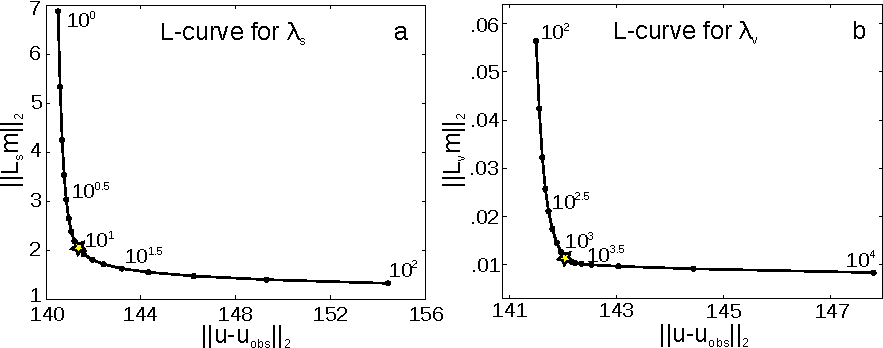
\includegraphics{ch2/figures/Fig2.pdf}
\caption{L-curves used to select the penalty parameters. Panel (a)
shows the trade-off between slip smoothness and data misfit while
varying $\lambda_s$ and keeping $\lambda_v$ fixed at zero.  Panel (b)
shows the trade off between smoothness of inferred viscosity and
misfit while varying $\lambda_v$ and keeping $\lambda_s$ fixed at the
value chosen from Panel (a).  Stars indicate our chosen penalty
parameters.}
\label{figure2}
\end{figure}

\section{Synthetic test}\label{SynthTest}
We demonstrate with two synthetic tests that our inverse method is
capable of recovering fault slip and an effective lithospheric
viscosity from postseismic deformation.  We use the finite element
software, PyLith \citep{Aagaard2013}, to compute the surface deformation
resulting from a specified amount of slip on a fault in a lithosphere
with either Maxwell or Burgers viscoelasticity.  We invert this
synthetic surface deformation using the method described above to
recover the imposed model parameters.  The synthetic tests also serve
to demonstrate that eqs. (\ref{PostseismicInitialVelocity}) and
(\ref{Postseismic_Approximation}) are indeed valid for three
dimensional earthquake models.

Our synthetic models consist of a 50 km long by 20 km wide strike-slip
fault, striking to the north and dipping $60^{\circ}$ to the east
(Fig. 5). At $t=0$ we impose $6.5\times 10^{19}$ N m of surface
rupturing, right-lateral coseismic slip with a distribution shown in
Fig. 3. After the coseismic slip, we impose 2 years of afterslip just
below the coseismic rupture zone.  The spatial distribution of
afterslip on the fault remains constant throughout the 2 years but the
rate of afterslip decreases by a factor of 2 every 0.5 years.  The
cumulative moment of afterslip over the first year is about $1.6\times
10^{19}$ N m, while the cumulative moment of afterslip over the second
year is $4.0\times 10^{18}$ N m.  We do not impose any fault slip
beyond $t=2$ years.

We compute surface displacements at 50 randomly chosen observation
points within a 400 km square centered about the fault (Fig. 5), which
is intended to roughly correspond with the density of GPS station at a
well instrumented plate boundary.  Displacements are computed at 0.05
year intervals up until $t=10$ years.  We add temporally correlated
noise to the computed displacements through time, consistent with what
one would expect from GPS observations.  The standard deviation of
northing and easting displacements is 1 mm, and the standard deviation
of the vertical displacements is 2.5 mm.  We add temporal covariance
with an exponential noise model that has a characteristic timescale of
0.25 years, which is intended to simulate seasonal processes that are
typically present in GPS time series.

\subsection{Green's functions}\label{GreensFunc}
We invert the synthetic surface displacements for fault slip on a 4 km
by 4 km discretization of the planar fault.  We estimate a constant
viscosity in 10 km thick horizontal layers from the surface down to 70
km depth and for a lower substrate. We compute the elastic Green's
functions, $F_i(\vec{x})$, and initial viscoelastic Green's functions,
$G_{ij}(\vec{x})$, numerically using PyLith.  The elastic Green's
functions are the initial surface displacements resulting from 1 m of
imposed slip on fault patch $i$.  For each fault patch, we use basis
slip directions with rake $45^\circ$ up-dip and $45^\circ$ down-dip of
pure right-lateral slip.  These slip basis directions restrict all
inferred slip to have rakes within $45^\circ$ of right-lateral. We
find the initial viscoelastic Green's functions, $G_{ij}(\vec{x})$, by
computing the initial rate of surface deformation due to 1 m of slip
on fault patch $i$ in a model that is elastic everywhere except in
region $j$, which is assigned a unit fluidity.  In the interests of
numerical stability we used $10^{-18}$ Pa$^{-1}$ s$^{-1}$ as our unit
of fluidity.  We emphasize that the amount we perturb the fluidity in
region $j$ will have no influence on our computation of $G_{ij}(x)$
because the initial rate of deformation computed with Pylith will be
proportional to $G_{ij}(x)$ times our fluidity perturbation.

We define the basis slip functions, $A_k(t)$, as a Heaviside function
centered at $t=0$ and twenty ramp functions which describe 1 m of
cumulative slip over the time intervals $t = (0,0.5), (0.5,1.0),
\dots,$ and $(9.5,10.0)$ years. We note that the synthetic model does
not have any fault slip from $t=2$ to 10 years and the postseismic
deformation over that interval is resulting purely from viscoelastic
creep.

\subsection{Synthetic model with Maxwell viscoelasticity}\label{MaxModel}

\begin{figure}
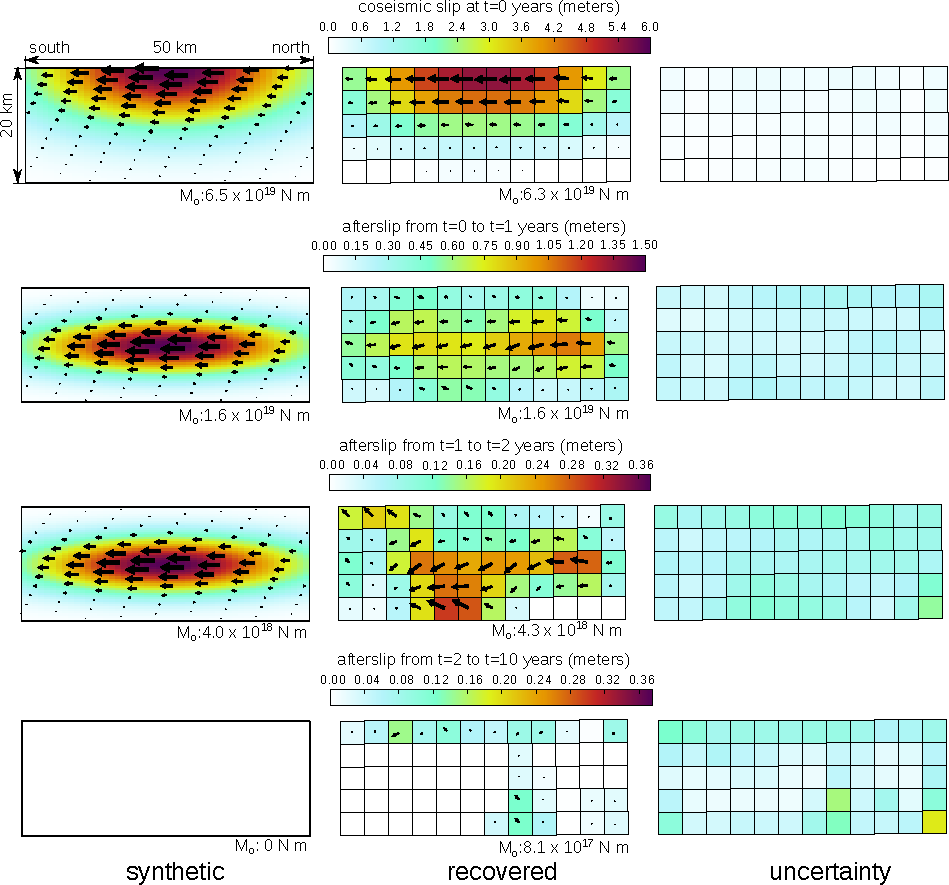
\includegraphics{ch2/figures/Fig3.pdf}
\caption{Slip distribution imposed in both synthetic models (left),
slip recovered for the synthetic model with Maxwell viscoelasticity
(middle), and uncertainty in the recovered slip magnitude (right).
Colors indicate magnitude of slip and arrows indicate direction of
slip (arrows pointing right indicate left-lateral and up is thrust).
The panels showing afterslip display cumulative slip over the
specified time interval.  The slip uncertainties are the standard
deviation of inferred slip magnitude during the specified period,
which were derived from 100 iterations of bootstrapping.}
\label{figure3}
\end{figure}

\begin{figure}
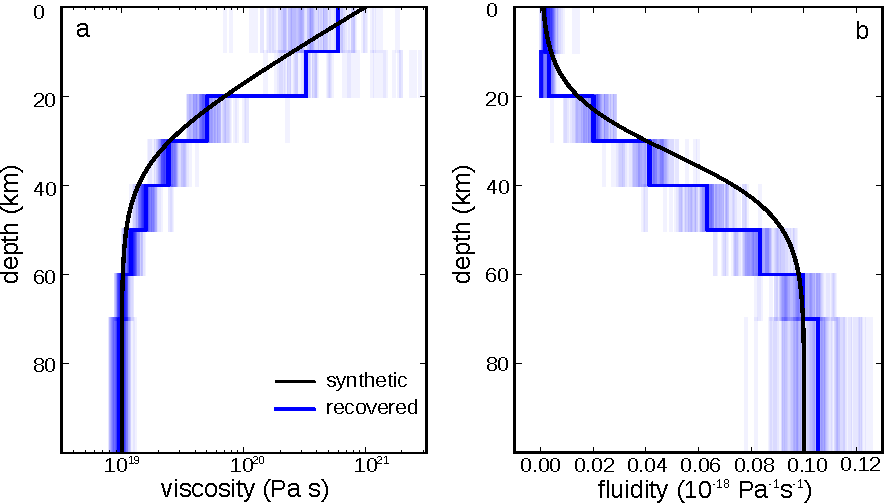
\includegraphics{ch2/figures/Fig4.pdf}
\caption{Synthetic and recovered lithospheric viscosities (left) and
associated fluidities (right).  Semi-transparent lines are recovered
models found through bootstrapping and indicate the degree of
uncertainty on the inferred viscosity structure.}
\label{figure4}
\end{figure}

\begin{figure}
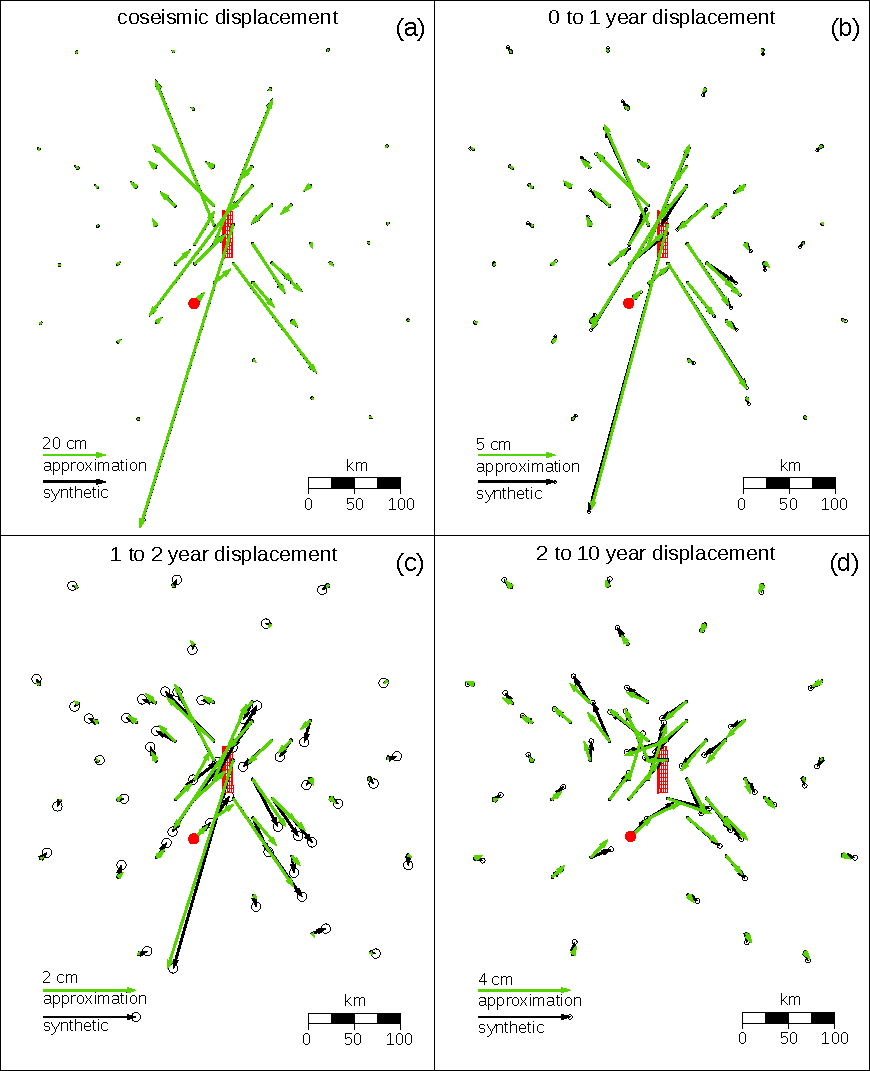
\includegraphics{ch2/figures/Fig5.pdf}
\caption{Synthetic surface displacements (black) and best fitting
surface displacements using eq. (\ref{Postseismic_Approximation2})
(green).  Vertical displacements are used in the inversion but are not
shown here. Panel (a) shows coseismic displacements and the remaining
panels show the cumulative displacements over the indicated time
intervals. Ellipses indicate 1 standard deviation uncertainty in the
synthetic data. Red dot indicates the position of the time series
shown in Fig. 6 and Fig. 9. The surface projection of the discretized
synthetic fault is depicted in red.}
\label{figure5}
\end{figure}

The lithosphere in our first synthetic model is Maxwell viscoelastic
with homogeneous Lam\'e parameters $\lambda = 32$ GPa and $\mu = 32$
GPa.  The viscosity in the lithosphere decays from $10^{21}$ Pa s
($\tau\approx1,000$ years) at the surface to $10^{19}$ Pa s
($\tau\approx10$ years) at 75 km depth (Fig. 4).  For the timescales
of this synthetic test, the uppermost lithosphere is effectively
elastic.

We use the penalty parameters chosen in Fig. 2 and our recovered model
of slip on the fault is shown in Fig. 3.  We use 100 iterations of
bootstrapping to assess how sensitive our recovered model is to the
imposed data noise.  The standard deviation of coseismic slip and
cumulative afterslip over the indicated interval is shown in the right
column of Fig. 3.  The spatial distribution and direction of inferred
coseismic slip are a good match to the synthetic coseismic slip.  The
distribution of afterslip was decently recovered but not as well as
the coseismic slip was recovered. Inferred afterslip over the first
year is smoother than the true slip due to the regularization,
although there is a high concentration of slip on the northern portion
of the fault which is consistent with the synthetic model.  We
attribute the better resolved northern portion of the fault to a
proximal surface observation point.  There are a few artifacts in the
distribution of inferred afterslip from $t=1$ to 2 years which are not
present in the synthetic model, such as slip on the deepest portion of
the fault. Our inability to recover the details of the imposed
afterslip as well as the coseismic slip could be because the data
noise is obscuring some of the postseismic signal (Fig. 5b and 5c
compared to Fig. 5a) and causing higher variability in inferred slip
models. Nevertheless, the inferred moment of both coseismic slip and
afterslip, which is proportional to slip integrated over the fault
plane, is within 10\% of the moment in the synthetic model.  Although
the spatial distribution of inferred slip may be more difficult to
recover, the slip moment seems to be consistently recovered.

The inferred slip over the last time interval, $t=2$ to 10 years, is
also consistent with the synthetic model.  The moment of slip over
this interval is $8.1\times 10^{17}$ N m, which is two orders of
magnitude smaller than the moment for the coseismic slip in the
synthetic model and is accounting for, at most, a few mm's of surface
displacement from $t=2$ to 10 years, which is on order of the data
uncertainty. We can further dismiss inferred afterslip during this
period as being negligibly small because the magnitude of inferred
slip is on order of the the uncertainty inferred from bootstrapping
(Fig. 3).  The majority of surface deformation during this time
interval (Fig. 5d) is therefore being properly attributed to
viscoelastic relaxation in the inversion results.

The inferred viscosities in each of the eight layers are shown in
Fig. 4(a).  The recovered viscosities correspond well with the
synthetic model.  The uncertainties of the recovered viscosities are
inferred using bootstrapping and we find that the strongest layers
near the surface, despite being close to the earthquake source,
have the highest uncertainties.  However, viscosities greater than
$~10^{20}$ Pa s are effectively elastic on the timescales of this
synthetic test and so a wide range of high viscosities for the upper
layers would just as adequately be able to describe the synthetic
surface displacements.  When looking at inferred values of fluidity
(Fig. 4b), we see that the uncertainties are lowest at the surface and
increase with depth, as is perhaps more intuitive.

Viscoelastic relaxation immediately below the fault and afterslip on
the fault would have similar surface manifestations, and thus it is
reasonable to explore the trade-off between these processes.  We use
the collection of models obtained through bootstrapping and compute
the correlation coefficient between the estimates of cumulative
afterslip moment over 10 years and the inferred fluidity for select
layers. Not surprisingly, the correlation coefficient is -0.16, and
-0.25 in the layer from 10 to 20 km depth and 20 to 30 km depth,
respectively, which means that higher estimates of fluidities in those
layers tend to be compensated by lower estimates of slip on the fault.
Interestingly, there is a positive correlation of 0.38 between
cumulative afterslip moment and the fluidity in the uppermost layer
containing the fault. The positive correlation is because deformation
resulting from viscoelastic relaxation in the uppermost layer
containing the fault tends to be in the opposite direction as deformation
resulting from fault slip. This means that a high fluidity in the
uppermost layer will tend to produce deformation that is balanced out by
higher amounts of slip.  It is conceivable that such a correlation
could lead to unrealistic inferences of viscosity in the near surface
and it may be necessary to assume that viscous regions containing a
fault are elastic.  There is no significant correlation between
afterslip and fluidity in layers below 30 km depth.

\subsubsection{Validation}\label{Validation}

\begin{figure}
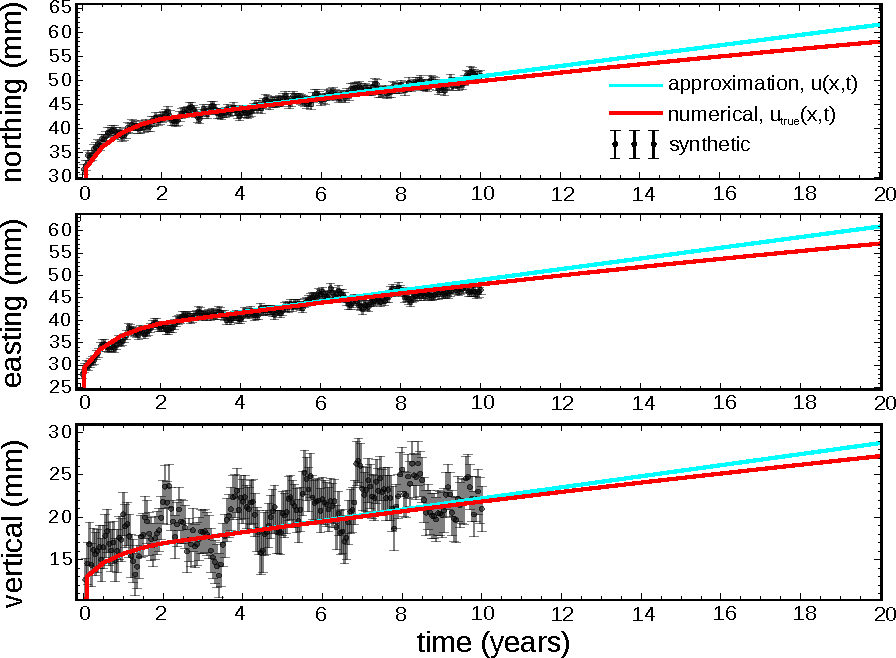
\includegraphics{ch2/figures/Fig6.pdf}
\caption{Displacement time series for the position shown in Fig. 5
(black), best fitting surface displacements using the approximation
from eq. (\ref{Postseismic_Approximation2}) (green) and surface
displacements computed with PyLith using the inferred slip
distribution and viscosity structure (red). Coseismic displacements at
$t=0$ are not shown.}
\label{figure6}
\end{figure}

\begin{figure}
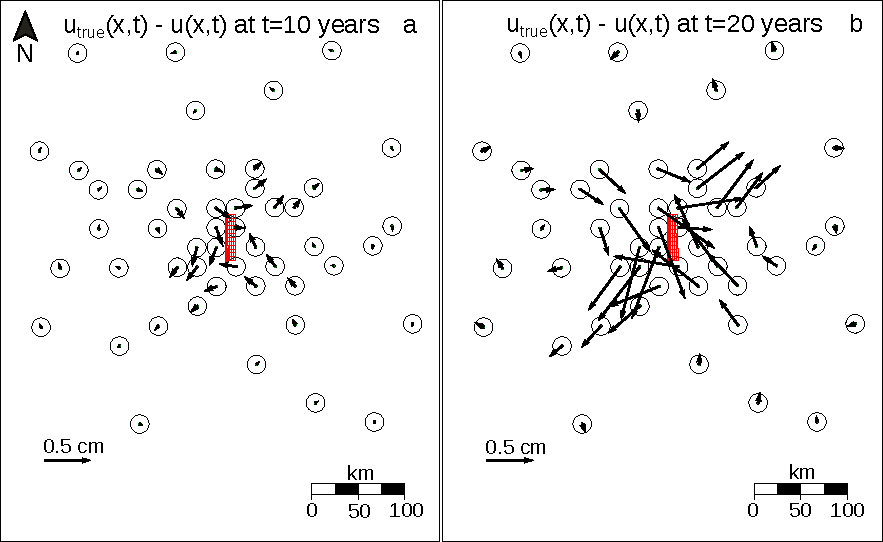
\includegraphics{ch2/figures/Fig7.pdf}
\caption{Approximation error at $t=10$ years and $t=20$ years. Circles
with 1 mm radius are centered at each station to compare the accuracy
of $\vec{u}(\vec{x},t)$ to the noise in the synthetic data.}
\label{figure7}
\end{figure}

The fact that our recovered fault slip and lithospheric viscosity are
in good agreement with the synthetic model suggests that the
approximation given by eq. (\ref{Postseismic_Approximation2}) is
accurate over the 10 years of synthetic data.  We further assess the
accuracy of eq. (\ref{Postseismic_Approximation2}) by running a
forward model with PyLith where the imposed fault slip and
lithospheric viscosity are those estimated from the synthetic data.
We then compare the displacements from the numerically computed
forward model with the displacements predicted by
eq. (\ref{Postseismic_Approximation2}).  We refer to the numerically
computed displacements as $\vec{u}_{\mathrm{true}}(\vec{x},t)$ and the
displacements predicted by the approximation as $\vec{u}(\vec{x},t)$
(Fig. 6).  We refer to the difference between
$\vec{u}_{\mathrm{true}}(\vec{x},t)$ and $\vec{u}(\vec{x},t)$ as the
approximation error (Fig. 7). At $t=10$ years the approximation error
is on order of a few mm's for each location, which is the magnitude of
the data uncertainty.  Additionally, the approximation error is small
compared to the cm's of deformation resulting from viscoelastic
relaxation, indicating that eq. (\ref{Postseismic_Approximation2}) is
indeed a fair approximation up to $t=10$ years.  At $t=20$ years the
approximation error is about one cm in magnitude for near field sites,
indicating that the approximation has broken down in the near field by
this time, while the error is still on order of a few mm's for the far
field sites.  The faster divergence for the near field sites is
consistent with the comparison we made between the approximate and
true displacements for a two-dimensional, two layered earthquake model
in Section \ref{2D2LModel} (Fig. 1).

The accuracy of eq. (\ref{Postseismic_Approximation2}) is also
demonstrated in Fig. 6, which shows $\vec{u}(\vec{x},t)$ and
$\vec{u}_{\mathrm{true}}(\vec{x},t)$ at a sample site near the fault.
The numerical solution asymptotically approaches the rate of
deformation predicted by eq. (\ref{Postseismic_Approximation2}) as
time goes to zero, demonstrating that
eq. (\ref{PostseismicInitialVelocity}) accurately describes the
initial viscoelastic response.  Additionally, the magnitude of the
difference between $\vec{u}(\vec{x},t)$ and
$\vec{u}_{\mathrm{true}}(\vec{x},t)$ is smaller than the uncertainty
of our synthetic data throughout the time series, indicating that
eq. (\ref{Postseismic_Approximation2}) is appropriate for this
synthetic test.  For this site and other near field sites, the
approximation starts to break down at about $t=10$ years. The lowest
relaxation time in our synthetic lithosphere is also about 10 years
and so the duration over which eq. (\ref{Postseismic_Approximation2})
is accurate is longer than what we found in our analysis for a
two-dimensional, two layered earthquake model in Section \ref{2D2LModel}.

\subsection{Synthetic model with Burgers viscoelasticity}\label{BurgersModel}
In the above synthetic example, we conveniently picked the length of
our displacement time series to correspond with the shortest
relaxation time in the lithosphere.  If the length of the time series
is significantly shorter than the relaxation time of the lithosphere,
then eq. (\ref{Postseismic_Approximation2}) would be an appropriate 
approximation and fault slip would be accurately recovered, although
there would not be a significant amount of deformation resulting from
viscoelastic relaxation and so inferences of viscosity would have high
uncertainty.  When the length of the time series is significantly
longer than the shortest relaxation time of the lithosphere then the
approximation would not be accurate and we would see a notable misfit
in our best fitting prediction of the data. Here we use another
synthetic test to demonstrate an iterative approach to finding the
optimal time series duration. We also use this synthetic test to
demonstrate how fluidities inferred using our inverse method can be
used to constrain the viscous properties of a non-Maxwell viscoelastic
lithosphere.

We consider a synthetic model with the same fault geometry and
prescribed slip as the synthetic model described in Section \ref{MaxModel}, but
the lithosphere now has a Burgers rheology.  A Burgers rheology can be
modeled schematically as a Maxwell spring-dashpot system connected in
series with a Kelvin spring-dashpot system. There are five rheologic
parameters needed to describe a Burgers rheology, the first Lam\'e
parameter, $\lambda$, shear moduli of the Maxwell and Kelvin elements,
$\mu_m$ and $\mu_k$, and the viscosities of the Maxwell and Kelvin
elements, $\eta_m$ and $\eta_k$.  In this synthetic test, we set
$\mu_m=\lambda=32$ GPa and $\eta_m$ equal to the viscosity structure
from the synthetic model in Section \ref{MaxModel}.  We also set $\mu_k=\mu_m$
and $\eta_k=0.1\eta_m$ so the lowest kelvin relaxation time
($\eta_k/\mu_k$) in our synthetic model is 1 year (Fig. 8).

We use the same $F_i(\vec{x})$, $G_{ij}(\vec{x})$, and $A_k(t)$,
described in Section \ref{GreensFunc} and estimate an effective
Maxwell viscosity by using 0.5, 2.0 and 5.0 years of synthetic data.
Our inverse method allows us to estimate a single value of viscosity
for each discretized region of the lithosphere and so we are unable to
recover both $\eta_k$ and $\eta_m$.  Instead, our method allows us to
estimate an effective viscosity for a Burgers viscoelastic lithosphere
during the early postseismic period.  We demonstrate in our
supplementary IPython notebook that when assuming $\mu_m$ is equal to
the shear modulus used to construct $F_i(\vec{x})$ and
$G_{ij}(\vec{x})$ then the effective fluidity inferred using our
method, $1/\eta$, is equivalent to
\begin{equation}\label{EquivalentBurgers}
\frac{1}{\eta} = \left(\frac{1}{\eta_k} + \frac{1}{\eta_m}\right).
\end{equation}

The recovered viscosities for each time series duration are shown in
Fig. 8 and we show the moment of inferred afterslip as a function of
time in Fig. 9. The synthetic and predicted displacement time series
at the observation point indicated in Fig. 5 are shown in Fig. 10.  We
are able to accurately predict the synthetic displacements (red line
in Fig. 10) and recover the fluidities expected following
eq. (\ref{EquivalentBurgers}) when using a 0.5 year time series. The
relatively few number of observations constraining the fluidity
inferences leads to large uncertainties as indicated by the
distribution of bootstrapped models.  When we use 2 years of
displacements, exceeding the minimum Kelvin relaxation time in the
synthetic model, the best fitting predicted displacements are still a
good fit to the synthetic data (green line), but it is difficult to
discern whether some of the systematic misfit is due to the inability
of eq. (\ref{Postseismic_Approximation2}) to describe the transient
displacement or because of the temporal correlation of our added
noise.  The inferences of fluidity when using 2 years of displacement
are consistently off by a factor of 0.5.  The underestimation of
fluidity is then compensated by a slight overestimation of cumulative
fault slip (Fig. 9). Although the estimated fluidities are incorrect,
the relative strength of the different layers is well recovered.  When
using 5 years of synthetic deformation, the depth dependence of
fluidity no longer resembles the true depth dependence and the
inferred moment of afterslip is appreciably higher than what was
imposed in the synthetic model. Even though additional afterslip is
describing some of the transient viscoelastic deformation, there is
still a systematic misfit in the best fitting prediction to the 5 year
time series (Fig. 10) indicating that
eq. (\ref{Postseismic_Approximation2}) is not valid for that duration
of time.  The length of the time series used for our inverse method
should be just long enough so that the best fitting predictions to the
data do not have any systematic misfit.  It is difficult to
distinguish by the fit to the data whether the model recovered using a
0.5 year time series or a 2 year time series is a better estimate of
the true model, although one can easily run a forward calculation for
each of the recovered models to see how well they predict the later
deformation.

\begin{figure}
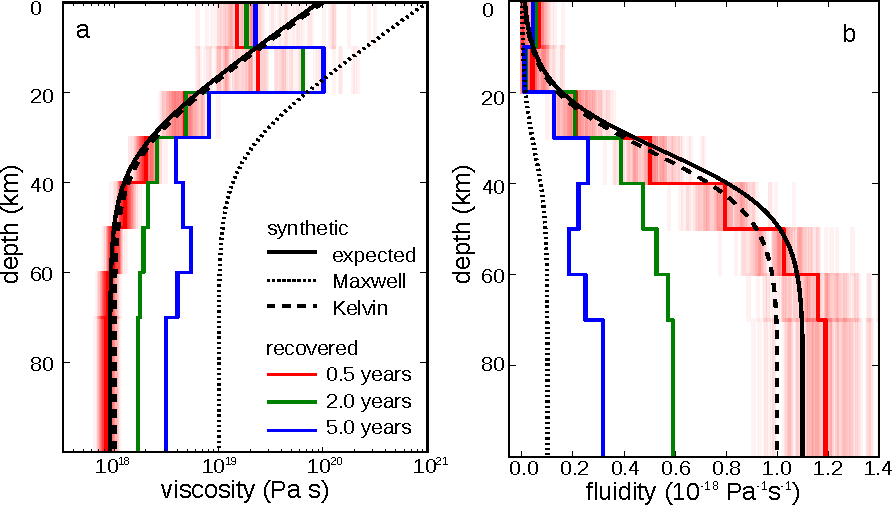
\includegraphics{ch2/figures/Fig8.pdf}
\caption{Synthetic and recovered lithospheric viscosities (left) and
fluidities (right) for the synthetic model with a Burgers rheology.
Dotted and dashed lines show the Maxwell and Kelvin viscosity in the
synthetic model, respectively.  The solid black line indicates the
effective viscosity from eq. (\ref{EquivalentBurgers}).  The red,
green, and blue lines show the inferred viscosities and fluidities
when inverting a 0.5, 2.0, and 5.0 year long time series,
respectively.  The light red lines are the bootstrapped fluidities and
viscosities inferred using the 0.5 year time series.}
\label{figure8}
\end{figure}

\begin{figure}
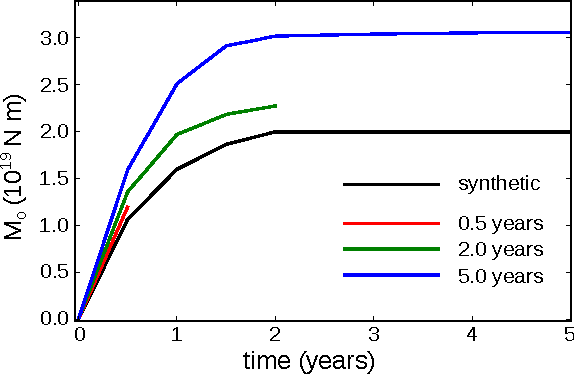
\includegraphics{ch2/figures/Fig9.pdf}
\caption{Afterslip moment over time for the synthetic model (black)
and the inferred afterslip moment when inverting 0.5, 2.0, and 5.0
years of displacements (red, green, and blue).}
\label{figure9}
\end{figure}

\begin{figure}
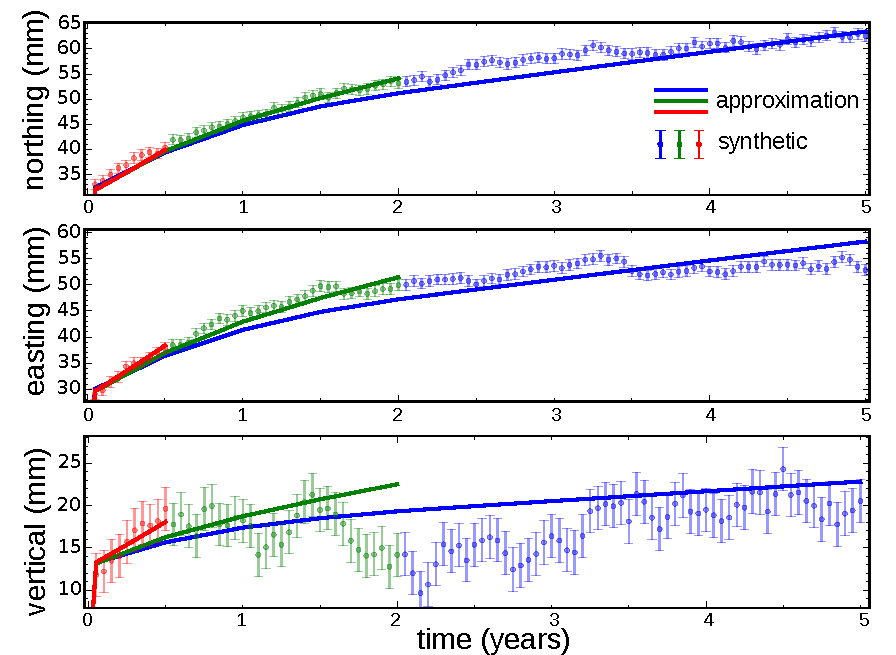
\includegraphics{ch2/figures/Fig10.pdf}
\caption{Synthetic and predicted displacement time series with
length 0.5, 2.0, and 5.0 years.  The time series shown is for the
observation point indicated in Fig 5.}
\label{figure10}
\end{figure}

\section{Discussion}
A fundamental assumption in our method for estimating slip and
viscosity from postseismic deformation is that the timescale of
relaxation in the weakest part of the lithosphere is at least as long
as the timescales over which postseismic deformation is observed.
This assumption allows us to approximate the surface expression of
viscous creep as a linear system with respect to lithospheric
fluidity, which greatly facilitates and expedites the inverse
problem. Since the relaxation times in a given region are generally
not well known \textit{a priori}, one must use an iterative approach as
described in Section \ref{BurgersModel} to determine the appropriate length of the time
series used in the inversion.  

We can look at previous studies to gauge the duration over which
our approximation would be accurate.  Surface deformation following large
($\geq M_w=7$) earthquakes often is characterized by transient and
rapid postseismic deformation in the first year after and earthquake
followed by steady deformation in later years
\citep[e.g.][]{Savage1997,Savage2005,Ergintav2009}.  Several studies have attributed
rapid early transient deformation following an earthquake to
afterslip, while describing the later steady deformation with viscous
relaxation in a Maxwell viscoelastic lower crust or upper mantle
\citep[e.g.][]{Perfettini2005,Johnson2009,Hearn2009,Freed2006a,Rollins2015}.  These studies have
found that lithospheric relaxation times no shorter than years or
decades are needed to describe postseismic deformation.  Indeed,
\citet{Perfettini2005} describes the trend in two years of postseismic
deformation following the 2001 $M_w=8.4$ Peru earthquake by assuming
that the lithospheric viscosity was sufficiently high that the rate of
deformation from viscoelastic creep could be considered constant,
which is the assumption that we make in formulating
eq. (\ref{Postseismic_Approximation}). If transient postseismic
deformation can be attributed to fault slip followed by steady
viscoelastic creep, then eq. (\ref{Postseismic_Approximation}) should
be able to describe displacements on the timescale of years or decades
after an earthquake.

Several studies have used rheologies containing a transient phase of
deformation to explain the early postseismic deformation.  For
example, \citet{Pollitz2003,Pollitz2005} invoked a Burgers rheology upper mantle
to explain surface displacements following the 2002 $M_w=7.9$ Denali
earthquake and the 1999 $M_w=7.1$ Hector Mine earthquake.  In both
cases the best fitting transient relaxation time was on the order of a
month and the best fitting steady-state relaxation time was on the
order of years.  Postseismic deformation following the Denali
earthquake was also successfully modeled by \citet{Freed2006b} with a
power-law rheology in the upper mantle, consistent with laboratory
studies \citep[e.g.][]{Kirby1987}.  The power-law rheology was able to
reproduce the observed transient surface deformation because the high
stresses in the earthquake decreased the effective viscosity of the
upper mantle to $\sim10^{17}$ Pa s resulting in fast surface
deformation.  As stresses from the earthquake relaxed, the effective
viscosity increased and the predicted surface deformation became
steadier. Based on the success of \citet{Pollitz2003,Pollitz2005} and
\citet{Freed2006b}, one may dismiss our method as being unrealistic
because we assume that the lithosphere is Maxwell viscoelastic.
However, our method does not necessarily preclude the possibility of a
Burgers rheology, as demonstrated in Section \ref{BurgersModel}, or a
stress-nonlinear viscosity.  As long as stresses in the lithosphere
remain roughly equal to the the stresses transferred elastically
through fault slip, then a viscosity structure inferred using our
method could be interpreted as the effective viscosity in a transient
viscoelastic or power-law rheology.  One could also use
eq. (\ref{EquivalentBurgers}) to constrain the rheologic properties
for a Burgers rheology.  If the commonly observed early transient
postseismic deformation truly is the result of viscous relaxation in
the lithosphere rather than afterslip, then the results from
\citet{Pollitz2003,Pollitz2005} and \citet{Freed2006b} suggest that the time interval
over which eq. (\ref{Postseismic_Approximation}) is appropriate is on
order of a month after an earthquake.  In such case, our method can be
used to get an initial estimate of lithospheric viscosity, while
unused portion of the displacement time series could be incorporated
in a gradient based nonlinear inverse method where the forward problem
is computed numerically rather than with
eq. (\ref{Postseismic_Approximation}).

Postseismic transient deformation could also be the result of creep in
a weak ductile shear zone which is embedded in a stronger viscoelastic
lithosphere \citep[e.g.][]{Hetland2014}. Sufficiently localized creep in a
shear zone can be modeled as slip on a down-dip extension of the
ruptured fault \citep[e.g.][]{Hearn2002,Kenner2003,Johnson2004} because the two
processes are kinematically indistinguishable.  Likewise,
\citet{Freed2006b} noted that deep fault slip could serve as a proxy for
distributed viscous relaxation in a weak lower crust when only
considering horizontal displacements. The applicability of our method
should therefore be unaffected by localized viscous deformation with
the understanding that inferences of fault slip could be absorbing
that deformation.


\section{Conclusion}
We present a method to invert coseismic and postseismic deformation to
simultaneously estimate a time dependent distribution of fault slip
and an arbitrarily discretized viscosity structure of the lithosphere.
We take advantage of an approximation for early postseismic
deformation resulting from fault slip and viscoelastic relaxation.
This approximation is computationally efficient which allows us to
rapidly search a high dimensional model space and make higher
resolution estimates of effective lithospheric viscosity than what can
feasibly be done with the commonly used grid search methods. Our
method is applicable for as long as this approximation is appropriate,
that is, for as long as stresses resulting from coseismic slip and
afterslip have not significantly decayed due to viscoelastic
relaxation.  Based on inferences of lithospheric viscosity from other
studies, we estimate that our method could be used for postseismic
deformation ranging from months to years after an earthquake.
Despite our methods application to a limited portion of the
postseismic period, we demonstrate that our method is capable of
robustly recovering the mechanisms driving postseismic deformation.


\bibliographystyle{agu04}
\bibliography{refs}

\newappendix{Appendix 2A: Inverse Laplace transform through series expansion}
Let $f(t)$ be analytic at $t=0$ and let there
  be a real valued $M$, and $C$ such that
\begin{equation}\label{constraints}
  \left|f^{(n)}(t)\right| < Ce^{Mt}\quad \forall t\geq 0\text{ and }\forall n\in\{0,1,2,\dots\},
\end{equation}
where $f^{(n)}(t)$ denotes the $n^{th}$ derivative of $f(t)$.  We
define the Laplace transform of $f(t)$ as
\begin{equation}
  \mathcal{L}[f(t)] := \hat{f}(s) := \int_{0}^\infty f(t)e^{-st}dt
\end{equation}
and we restrict our attention to $s\in\mathbb{R}$.  The constraints on
$f^{(n)}(t)$ from eq. (\ref{constraints}) ensure that
\begin{equation}\label{Property2}
  \lim_{s \to \infty}\mathcal{L}[f^{(n)}(t)] = 0.
\end{equation}
It can be shown using integration by parts that
\begin{equation}\label{Property1}
  \mathcal{L}[f^{(n)}(t)] = s^n\hat{f}(s) - \sum_{m=1}^ns^{m-1}f^{(n-m)}(0)
  \quad \forall s>M.
\end{equation}
Substituting eq. (\ref{Property1}) into eq. (\ref{Property2}) and then
rearranging the terms gives us a recursive formula for $f^{(n)}(0)$ in
terms of $\hat{f}(s)$:
\begin{equation}\label{NthDeriv}
  f^{(n)}(0) = \lim_{s \to \infty} s^{n + 1}\hat{f}(s) -
               \sum_{m=1}^{n} s^{m}f^{(n-m)}(0),
\end{equation}
where the base case, $n=0$, is the initial value theorem:
\begin{equation}\label{NthDerivBase}
  f(0) = \lim_{s \to \infty} s\hat{f}(s).
\end{equation}
Since we request $f(t)$ to be analytic at $t=0$, we can construct a
Taylor series expansion of $f(t)$ such that
\begin{equation}\label{TaylorSeries}
  f(t) = \sum_{n=0}^\infty\frac{f^{(n)}(0)}{n!}t^n
\end{equation}
for all values of $t$ within some neighborhood of $t=0$. We find the
inverse Laplace transform of $\hat{f}(s)$ by combining
eq. (\ref{TaylorSeries}) with eqs. (\ref{NthDeriv}) and
(\ref{NthDerivBase}) so that $f(t)$ is expressed in terms of
$\hat{f}(s)$.


\newappendix{Appendix 2B: Postseismic approximation for a two-dimensional earthquake model with a depth dependent viscosity}
We seek to find an approximation for early postseismic deformation in
a two-dimensional, strike-slip earthquake model with an arbitrary
depth-dependent viscosity below the fault locking depth, $D$.  We
first find the initial rate of surface deformation following a unit of
slip in a lithosphere that is elastic except for a viscoelastic layer
which is at depth $z$ and with thickness $\Delta z$. This is found by
making the substitutions $H_1 \to z$, $H_2 \to \Delta z$, $\eta_1 \to
\infty$, $\eta_3 \to \infty$, and $\eta_2 \to \eta$ in
eq. (\ref{ThreeLayerViscousResponse}), which gives us
\begin{equation}
  \frac{\partial}{\partial t}u_1(x,t)\big|_{t=0} = 
  \frac{1}{\eta}(W(z+\Delta z) - W(z)),
\end{equation}
where
\begin{equation}
  W(z) = \frac{\mu}{2\pi}\left(\tan^{-1}\left(\frac{2z-D}{x}\right) -
  \tan^{-1}\left(\frac{2z+D}{x}\right)\right).
\end{equation}
From eq. (\ref{PostseismicInitialVelocity}) we know that the initial
rate of surface deformation for a lithosphere composed of $N$ discrete
layers, each with viscosity $\eta_i$, at depth $z_i$, and having
thickness $\Delta z$, is then
\begin{equation}
  \frac{\partial}{\partial t}u_N(x,t)\big|_{t=0} = \sum_i^N
  \frac{1}{\eta_i}(W(z_i + \Delta z) - W(z_i)).
\end{equation}
The initial rate of surface deformation for a viscosity structure
given by $\eta(z)$ is found by taking the limit as $\Delta z \to 0$
and $N \to \infty$:
\begin{align}\label{ArbitraryViscousResponse}
 \frac{\partial}{\partial t}u(x,t)\big|_{t=0} &= \int_D^\infty
 \frac{1}{\eta(z)}\frac{\partial}{\partial z} W(z) dz\\
 &= \int_D^{\infty}\frac{\mu}{2\pi\eta(z)}\left(\frac{2x}{x^2 + \left(D + 2z\right)^2} -
                     \frac{2x}{x^2 + \left(2z - D\right)^2}\right) dz.
\end{align}
Finally, we add the elastic component of deformation and integrate
eq. (B.5) with the fault slip history to obtain
an approximation for early postseismic deformation:
\begin{equation}
u(x,t) \approx \frac{b(t)}{\pi}\tan^{-1}(\frac{D}{x}) + 
               \int_o^t\int_D^\infty \frac{\mu b(\theta)}{2\pi\eta(z)}
                                    \left(\frac{2x}{x^2 + \left(D + 2z\right)^2} - 
                                    \frac{2x}{x^2 + \left(2z - D\right)^2}\right)
                                    dz d\theta.
\end{equation}


\chapter
[Rheologic constraints on the upper mantle from five years of
postseismic deformation following the El Mayor-Cucapah earthquake]
{Rheologic constraints on the upper mantle from five years of
postseismic deformation following the El Mayor-Cucapah earthquake\footnote[1]{
This chapter has been published as: Hines, T. T., and Hetland, E. A.
(2016). Rheologic constraints on the upper mantle from five years of
postseismic deformation following the El Mayor-Cucapah earthquake.
Journal of Geophysical Research: Solid Earth, 121,
doi:10.1002/2016JB013114.}}

\section{Abstract}
We analyze five years of Southern California GPS data following the
Mw=7.2 El Mayor-Cucapah earthquake.  We observed transient postseismic
deformation which persists for three years at epicentral distances
greater than ${\sim}200$ km.  In the near-field, rapid postseismic
transience decays to a sustained rate which exceeds its preseismic
trend.  We attempt to determine the mechanisms driving this
deformation, where we consider afterslip at seismogenic depths and
viscoelastic relaxation in the lower crust and upper mantle as
candidate mechanisms.  We find that early, rapid, near-field
deformation can be explained with afterslip on the fault that ruptured
coseismically. The later, sustained, near-field deformation can be
explained with viscoelastic relaxation in the lower crust with a
steady-state viscosity of ${\sim}10^{19}$ Pa s and possibly continued
afterslip.  The postseismic deformation in the far-field is best
explained with a transient viscosity of ${\sim}10^{18}$ Pa s in the
upper mantle. We argue that a transient rheology in the mantle is
preferable over a Maxwell rheology because it better predicts the
decay in postseismic deformation, and also because it does not
conflict with the generally higher, steady-state viscosities inferred
from studies of geophysical processes occurring over longer time
scales.

\section{Introduction}
Ground deformation in the years following a large (Mw$\gtrsim$7)
earthquake can be used to gain insight into the mechanical behavior of
the crust and upper mantle. The interpretations of postseismic
deformation are not always conclusive because multiple postseismic
deformation mechanisms, such as afterslip or viscoelastic relaxation
in the lower crust and upper mantle, can have qualitatively similar
surface expressions \citep[e.g.,][]{Savage1990}. This non-uniqueness
complication can potentially be remedied if the postseismic
deformation occurs in an area that is sufficiently well instrumented
with GPS stations \citep{Hearn2003}.  Owing to the dense geodetic
network deployed throughout the 2000s as part of the Plate Boundary
Observatory, the postseismic deformation following the April 4, 2010,
Mw=7.2 El Mayor-Cucapah earthquake in Baja California was observed at
more GPS stations than any other earthquake in California to date (see
\citet{Hauksson2011} and \citet{Fletcher2014} for a detailed
description of this earthquake and its seismotectonic context).  With
such a large collection of data, we attempt to discern the mechanisms
driving the postseismic deformation. Previous studies which have
modeled postseismic deformation following the El Mayor-Cucapah
earthquake include \citet{Pollitz2012}, \citet{Gonzalez-ortega2014},
\citet{Spinler2015}, and \citet{Rollins2015}. Of these studies,
\citet{Gonzalez-ortega2014} and \citet{Rollins2015} have attempted to
describe the postseismic deformation with afterslip in an elastic
half-space.  \citet{Gonzalez-ortega2014} described five months of
postseismic deformation, observed by InSAR and GPS stations within
${\sim}50$ km of the rupture, with afterslip and contraction on the
coseismically ruptured fault. \citet{Gonzalez-ortega2014} noted that
their preferred model underestimated the GPS displacements for
stations $\gtrsim 25$ km from the rupture and suggested that it could
be the result of unmodeled viscoelastic relaxation.  Using only
continuous GPS stations, which are mostly north of the rupture zone,
\citet{Rollins2015} found that three years of postseismic deformation
can be adequately explained by afterslip, albeit with an implausibly
large amount of slip inferred on the least constrained, southern-most
fault segment. Here, we suggest the afterslip inferred by
\citet{Rollins2015} may have been acting as a proxy for distributed
relaxation in the upper mantle.

\citet{Pollitz2012}, \citet{Rollins2015} and \citet{Spinler2015}
explored viscoelastic relaxation in the lower crust and upper mantle
as a potential postseismic deformation mechanism. The rheology of the
crust and mantle is largely unknown and so modeling postseismic
deformation with viscoelastic relaxation requires one to assume a
rheologic model and then find the best fitting rheologic parameters.
The inference of these rheologic parameters is a computationally
expensive non-linear inverse problem which is typically approached
with a forward modeling grid search method.  Consequently, a
simplified structure for the Earth must be assumed in order to
minimize the number of rheologic parameters that need to be estimated.
For example, it is commonly assumed that the lower crust and upper
mantle are homogeneous, Maxwell viscoelastic layers, which may be too
simplistic for postseismic studies \citep{Riva2009,Hines2013}. To
further reduce the dimensions of the model space, it is also necessary
to make simplifying assumptions about the behavior of afterslip. For
example, one can assume a frictional model for afterslip and
parametrize afterslip in terms of the unknown rheologic properties of
the fault \citep[e.g.,][]{Johnson2009,Johnson2004}. One can also
assume that afterslip does not persist for more than a few months and
then model the later postseismic deformation assuming it to be the
result of only viscoelastic relaxation
\citep[e.g.,][]{Pollitz2012,Spinler2015}. However, afterslip in
similar tectonic settings has been observed to persist for decades
following earthquakes \citep{Cakir2012,Cetin2014}. Indeed, the
preferred viscoelastic model from \citet{Pollitz2012} significantly
underestimates deformation in the Imperial Valley, which could be
indicative of unmodeled continued afterslip.  Neglecting to allow for
sustained afterslip as a postseismic mechanism could then lead to
biased inferences of viscosities.

In this study, we perform a kinematic inversion for fault slip,
allowing it to persist throughout the postseismic period, while
simultaneously estimating the viscosity of the lower crust and upper
mantle.  We create an initial model of the fault slip and effective
viscosity necessary to describe early postseismic deformation using
the method described in \citet{Hines2016}.  This method uses a
first-order approximation of surface deformation resulting from
viscoelastic relaxation which is only applicable to the early
postseismic period. In this case, our initial model describes the
first 0.8 years of postseismic deformation following the El
Mayor-Cucapah earthquake.  We then use the inferred effective
viscosity structure from the initial model to create a suite of
postseismic models which we test against the five years of postseismic
data available to date.  Of the suite of models tested, we find that
postseismic deformation following the El Mayor-Cucapah earthquake can
be explained with a combination of afterslip on a fault segment
running through the Sierra Cucapah and viscoelastic relaxation in a
Zener rheology upper mantle with a transient viscosity on the order of
$10^{18}$ Pa s.

\begin{figure}
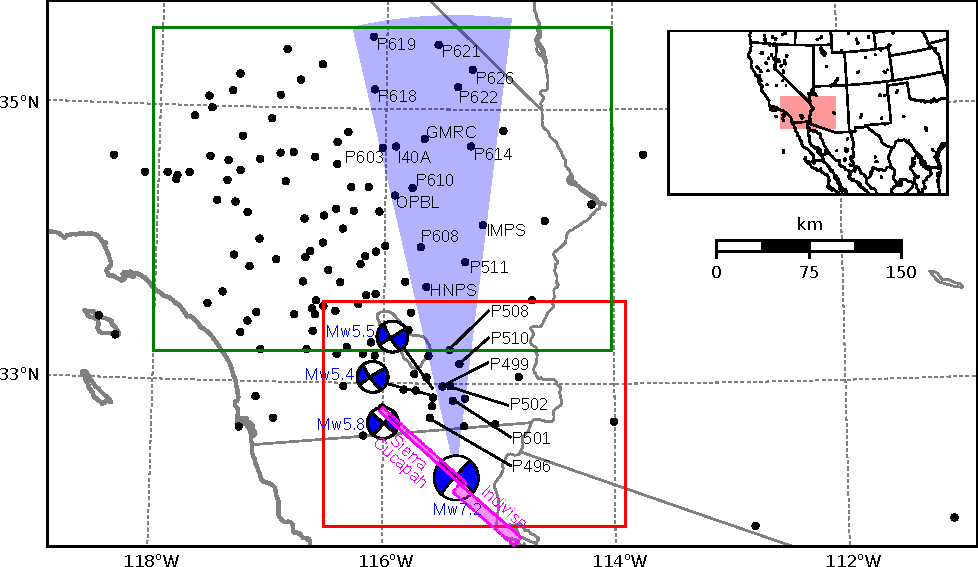
\includegraphics[scale=1.0]{ch3/figures/2016jb013114-p01} 
\caption
[Map of the region considered in this study]
{Map of the region considered in this study.  The large focal
mechanism is the GCMT solution for the El Mayor-Cucapah earthquake,
and the three small focal mechanisms are for the Ocotillo earthquake
and the two main shocks during the Brawley swarm.  The black dots
indicate the locations of GPS stations used in this study.  The fault
geometry used in this study is shown in magenta where dashed lines
indicate buried edges of the fault segments.  The green and red boxes
demarcate the extent of the near-field and far-field maps (Figures
\ref{ch3:fig:NearField} and \ref{ch3:fig:FarField}).  Stations inside
the blue sector, which highlights the area within 10$^\circ$ of the El
Mayor-Cucapah P-axis, are used in Figures
\ref{ch3:fig:RecordSectionMain} and \ref{ch3:fig:RecordSection1}.}
\label{ch3:fig:ContextMap}
\end{figure}

\section{Data processing}\label{ch3:sec:Data}
We use continuous GPS position time series provided by University
Navstar Consortium (UNAVCO) for stations within a 400 km radius about
the El Mayor-Cucapah epicenter. We collectively describe the coseismic
and postseismic displacements resulting from the El Mayor-Cucapah
earthquake as $u_\mathrm{post}(t)$.  We consider the GPS position time
series, $u_\mathrm{obs}(t)$, to be the combination of
$u_\mathrm{post}(t)$, secular tectonic deformation, annual and
semi-annual oscillations, and coseismic offsets from significant
earthquakes over the time span of this study.  The June 14, 2010,
Mw=5.8 Ocotillo earthquake and the Brawley swarm, which included an
Mw=5.5 and an Mw=5.4 event on August 26, 2012 (Figure
\ref{ch3:fig:ContextMap}), are the only earthquakes that produced
noticeable displacements in any of the time series.  We treat the
displacements resulting from the Brawley swarm as a single event
because the daily solutions provided by UNAVCO cannot resolve the
separate events.  Although the Ocotillo earthquake had its own series
of aftershocks \citep{Hauksson2011}, neither the Ocotillo earthquake
nor the Brawley swarm produced detectable postseismic deformation.  We
model displacements resulting from these events with only a Heaviside
function, $H(t)$, describing the coseismic offsets.  We then model
$u_\mathrm{obs}(t)$ as
\begin{equation}
  u_\mathrm{obs}(t) = u_\mathrm{pred}(t) + \epsilon,
\end{equation}
where
\begin{equation}\label{TimeSeriesModel}
  \begin{split}  
    u_\mathrm{pred}(t) = &u_\mathrm{post}(t)H(t-t_\mathrm{emc}) + c_0 + c_1t + \\
                         &c_2\sin(2\pi t) + c_3\cos(2\pi t) + c_4\sin(4\pi t) + c_5\cos(4\pi t) + \\
                         &c_6H(t-t_\mathrm{oc}) + c_7H(t-t_\mathrm{bs}).
  \end{split}
\end{equation}
In the above equations, $t_\mathrm{emc}$, $t_\mathrm{oc}$ and
$t_\mathrm{bs}$ are the times of the El Mayor-Cucapah earthquake,
Ocotillo earthquake, and the Brawley swarm, respectively, $c_0$
through $c_7$ are unknown coefficients, and $\epsilon$ is the
observation noise.  We are using years as our unit of time which makes
$c_2$ through $c_5$ the coefficients for annual and semi-annual
oscillations.  We only estimate jumps associated with the Ocotillo
earthquake and Brawley swarm for stations within 40 km of their
epicenters.

Stations which recorded displacements that clearly cannot be described
by the aforementioned processes are not included in our analysis. This
includes stations in the Los Angeles basin, where anthropogenic
deformation can be larger than the postseismic signal that we are
trying to estimate \citep{Bawden2001,Argus2005}. In order to ensure an
accurate estimation of the secular deformation, we only use stations
that were installed at least six months prior to El Mayor-Cucapah
earthquake even though several GPS stations were installed after the
earthquake to get better coverage of the postseismic deformation field
\citep{Spinler2015}.  It would be possible to subtract secular
velocities derived from elastic block models
\citep[e.g.,][]{Meade2005} from velocities recorded at the newly
installed stations to get an estimate of postseismic velocities at
those stations. However, estimating velocities from an already noisy
displacement time series can introduce significant uncertainties
depending on exactly how the estimation is done.  We therefore use
coseismic and postseismic displacements, rather than velocities, in
our inverse method described in Section \ref{ch3:sec:Model}. This
choice prevents us from using the newly installed stations for our
analysis.

The October 16, 1999, Mw=7.1 Hector Mine earthquake, which occurred
${\sim}270$ km north of the El Mayor-Cucapah epicenter, produced
transient postseismic deformation which we do not wish to model,
either mechanically or through empirical line fitting.  We thus
restrict our analysis to deformation observed six years after the
Hector Mine earthquake, which is when postseismic velocities at sites
near the Hector Mine epicenter are approximately constant
\citep{Savage2009}. When appraising our model fit in Section
\ref{ch3:sec:Model}, we see some systematic residuals in the vicinity
of the Hector Mine epicenter, which may be the result of errors in the
assumption that the trend in Hector Mine postseismic deformation is
linear after six years.

Studies of postseismic deformation typically assume a parametric form
for $u_\mathrm{post}(t)$, such as one with a logarithmic or
exponential time dependence \citep[e.g.,][]{Savage2005a}.  However, by
assuming a logarithmic or exponential form of $u_\mathrm{post}(t)$ we
run the risk of over fitting the GPS time series and inferring a
non-existent postseismic signal. We therefore do not assume any
parametric form for $u_\mathrm{post}(t)$ and rather treat it as
integrated Brownian motion, so that
\begin{equation}
    \dot{u}_\mathrm{post}(t) = \sigma^2\int_0^t w(s) ds,
\end{equation}    
where $w(t)$ is white noise and the variance of
$\dot{u}_\mathrm{post}(t)$ increases linearly with time by a factor of
$\sigma^2$. We use a Kalman filtering approach to estimate
$u_\mathrm{post}(t)$ and the unknown parameters in eq.
(\ref{TimeSeriesModel}).  In the context of Kalman filtering, our time
varying state vector is
\begin{equation}
    \mathbf{X}(t) = [u_\mathrm{post}(t),\dot u_\mathrm{post}(t), c_0, ..., c_7]
\end{equation}
and eq. (\ref{TimeSeriesModel}) is the observation function which maps
the state vector to the GPS observations. We initiate the Kalman
filter by assuming a prior estimate of $\mathbf{X}(t)$ at the first
time epoch, denoted $\mathbf{X}_{1|0}$, which has a sufficiently large
covariance, denoted $\mathbf{\Sigma}_{1|0}$, to effectively make our
prior uninformed.  For each time epoch, $t_i$, Bayesian linear
regression is used to incorporate GPS derived estimates of
displacement with our prior estimate of the state,
$\mathbf{X}_{i|i-1}$, to form a posterior estimate of the state,
$\mathbf{X}_{i|i}$, which has covariance $\mathbf{\Sigma}_{i|i}$.  We
then use the posterior estimate of the state at time $t_i$ to form a
prior estimate of the state at time $t_{i+1}$ through the transition
function
\begin{equation}\label{predict}
  \mathbf{X}_{i+1|i} = \mathbf{F}_{i+1}\mathbf{X}_{i|i} + \mathbf{\delta}_{i+1}, 
\end{equation}
where 
\begin{equation}
  \mathbf{F}_{i+1} = 
  \left[
  \begin{array}{ccc}
    1           & (t_{i+1} - t_i) & \mathbf{0}\\
    0           & 1              & \mathbf{0}\\
    \mathbf{0}  & \mathbf{0}     & \mathbf{I}
  \end{array}
  \right]
\end{equation}
and $\mathbf{\delta}_{i+1}$ is the process noise, which has zero mean
and covariance described by
\begin{equation}
  \mathbf{Q}_{i+1} = 
  \sigma^2 \left[
  \begin{array}{ccc}
  \frac{(t_{i+1} - t_i)^3}{3} & \frac{(t_{i+1} - t_{i})^2}{2} & \mathbf{0}\\
  \frac{(t_{i+1} - t_i)^2}{2} & (t_{i+1} - t_{i}) & \mathbf{0}\\ 
  \mathbf{0} & \mathbf{0} & \mathbf{0}
  \end{array}
  \right].
\end{equation}
The covariance of the new prior state, $\mathbf{X}_{i+1|i}$, is then
described by
\begin{equation}
  \mathbf{\Sigma}_{i+1|i} = \mathbf{F}_{i+1}\mathbf{\Sigma}_{i|i}\mathbf{F}^T_{i+1} + \mathbf{Q}_{i+1}.
\end{equation}
This process is repeated for each of the $N$ time epochs.  We then use
Rauch-Tung-Striebel smoothing \citep{Rauch1965} to find
$\mathbf{X}_{i|N}$, which is an estimate of the state at time $t_i$
that incorporates GPS observation for all $N$ time epochs.  Our final
estimates of $u_\mathrm{post}(t)$ are used in subsequent analysis,
while the remaining components of the state vector are considered
nuisance parameters. In the interests of computational tractability,
we down sample our smoothed time series from daily solutions down to
weekly solutions.

The smoothness of $u_\mathrm{post}(t)$ is controlled by the chosen
value of $\sigma$, which describes how rapidly we expect postseismic
displacements to vary over time.  Setting $\sigma$ equal to zero will
effectively result in modeling $u_\mathrm{post}(t)$ as a straight line
which is insufficient to describe the expected transient behavior in
postseismic deformation. The other end member, where $\sigma$ is
infinitely large, will result in $u_\mathrm{pred}(t)$ overfitting the
data. While one can use a maximum likelihood based approach for
picking $\sigma$ \citep[e.g.,][]{Segall1997}, we instead take a
subjective approach and choose a value for $\sigma$ that is just large
enough to faithfully describe the observed deformation at the most
near-field station in our study, P496, which exhibits the most rapid
changes in velocity. This ensures that $\sigma$ will be sufficiently
large so that our estimate of $u_\mathrm{post}(t)$ does not smooth out
potentially valuable postseismic signal at the remaining stations. We
find that using $\sigma = 50\ \mathrm{mm}/\mathrm{yr}^{1.5}$
adequately describe all but the first week of postseismic deformation
at station P496, which slightly increases our estimate of coseismic
displacements (Figure \ref{ch3:fig:P496}).  We include an example of
estimating $u_\mathrm{post}(t)$ for a far-field station, P619, which
is about 359 km north of the El Mayor-Cucapah epicenter (Figure
\ref{ch3:fig:P619}).  At station P619, along with all the other
stations in the Mojave region, there is a south-trending postseismic
transience that persists for the first three years after the El
Mayor-Cucapah earthquake.  Postseismic deformation that extends to
these epicentral distances has also been observed after the Hector
Mine earthquake \citep{Freed2007a}.

\begin{figure}
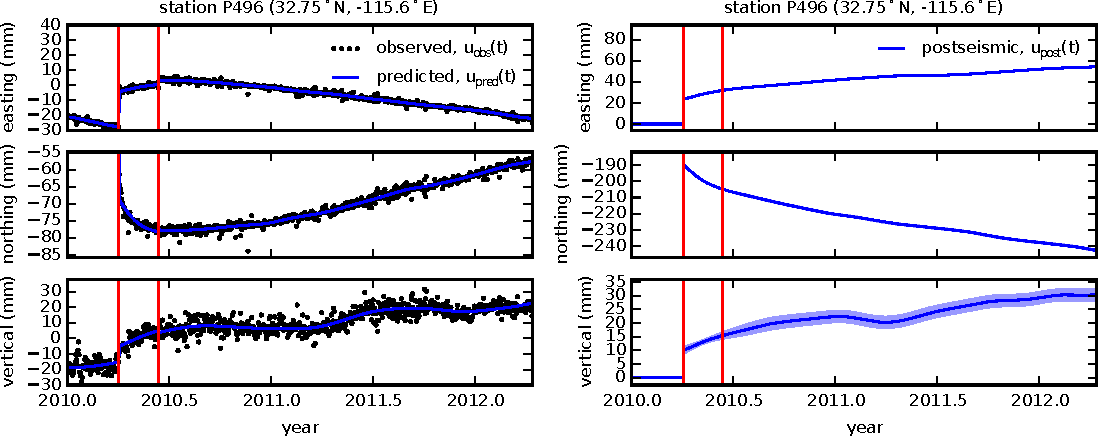
\includegraphics[scale=0.9]{ch3/figures/2016jb013114-p02}
\caption
[Observed displacements and estimated postseismic displacements
for station P496] 
{Left panels show GPS time series from UNAVCO (black) and the
predicted displacement (blue) from eq. (\ref{TimeSeriesModel}) for a
near-field station.  Red lines indicate the times of the El
Mayor-Cucapah and Ocotillo earthquake. The right panels show estimated
coseismic and postseismic displacements, $u_\mathrm{post}$, which are
extracted from the predicted displacements.  The 68\% confidence
interval is shown in light blue.}
\label{ch3:fig:P496}
\end{figure}

\begin{figure}
\noindent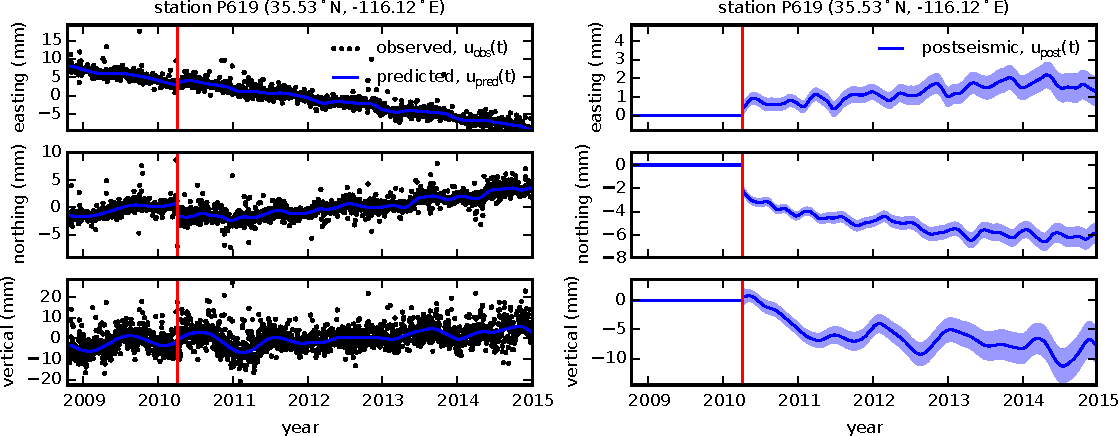
\includegraphics[scale=0.9]{ch3/figures/2016jb013114-p03}
\caption
[Observed displacements and estimated postseismic displacements
for station P619] 
{same as Figure \ref{ch3:fig:P496} but for a far-field station.} 
\label{ch3:fig:P619}
\end{figure}

It is important to note that the shown uncertainties in
$u_\mathrm{post}(t)$ do not account for the non-negligible epistemic
uncertainty in eq. (\ref{TimeSeriesModel}).  For example, we assume a
constant rate of secular deformation, which appears to be an
appropriate approximation for all but perhaps the stations closest to
the Hector Mine epicenter, as noted above.  Also, our model for
seasonal deformation in eq. (\ref{TimeSeriesModel}) assumes a constant
amplitude over time, which means that any yearly variability in the
climatic conditions could introduce systematic residuals
\citep{Davis2012}. Indeed, it would be more appropriate to consider
the seasonal amplitudes $c_2-c_5$ in eq. (\ref{TimeSeriesModel}) as
stochastic variables \citep{Murray2005}. By using constant seasonal
amplitudes, our estimate of $u_\mathrm{post}(t)$ seems to describe
some of the unmodeled annual and semi-annual oscillations (e.g. Figure
\ref{ch3:fig:P619}).

We show in Figures \ref{ch3:fig:NearField} and \ref{ch3:fig:FarField}
the near and far-field coseismic displacements and the postseismic
displacements accumulated over the time intervals 0-1 years, 1-3
years, and 3-5 years.  Stations at epicentral distances beyond
${\sim}200$ km have an elevated rate of deformation for the first
three years following the earthquake.  This far-field deformation is
trending southward at a rate of a few millimeters per year along the
direction of the El Mayor-Cucapah P-axis.  A similar eastward trend
can be seen in the few far-field stations in Arizona, located along
the T-axis.  After three years, the trend in far-field postseismic
deformation is barely perceptible.  Most far-field stations display an
initial subsidence for the first year after the El Mayor-Cucapah
earthquake followed by continued uplift.  This trend in vertical
deformation can be observed in all three of the quadrants where
postseismic data is available, which means that the vertical
deformation does not exhibit an anti-symmetric quadrant pattern, as
would be expected for postseismic processes.  Although we use vertical
deformation in our analysis in Section \ref{ch3:sec:Model}, we do not
put an emphasis on trying to describe the vertical deformation because
it likely does not have postseismic origins.

\begin{figure}
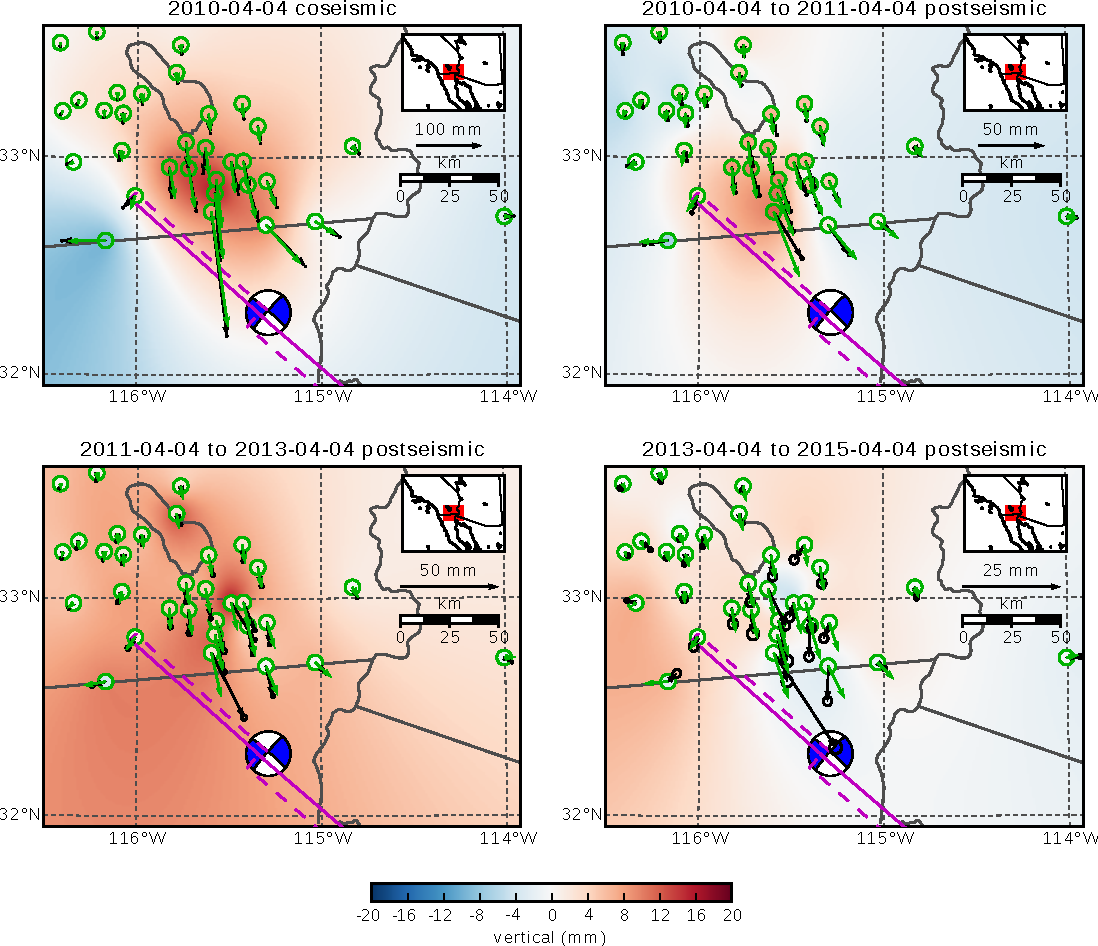
\includegraphics[scale=0.9]{ch3/figures/2016jb013114-p04}
\caption
[Observed and predicted near-field postseismic deformation]
{Near-field coseismic and cumulative postseismic displacements
over the indicated time periods (black) and predicted displacements
for our preferred model from Section \ref{ch3:sec:FullInversion}
(green).  The black error ellipses show the 68\% confidence interval
for the observed horizontal displacements.  Observed vertical
displacements are shown as an interpolated field and predicted
vertical displacements are shown within the green circles.  Note that
the interpolant is not well constrained in Mexico where there is no
data available.}
\label{ch3:fig:NearField}
\end{figure}

\begin{figure}
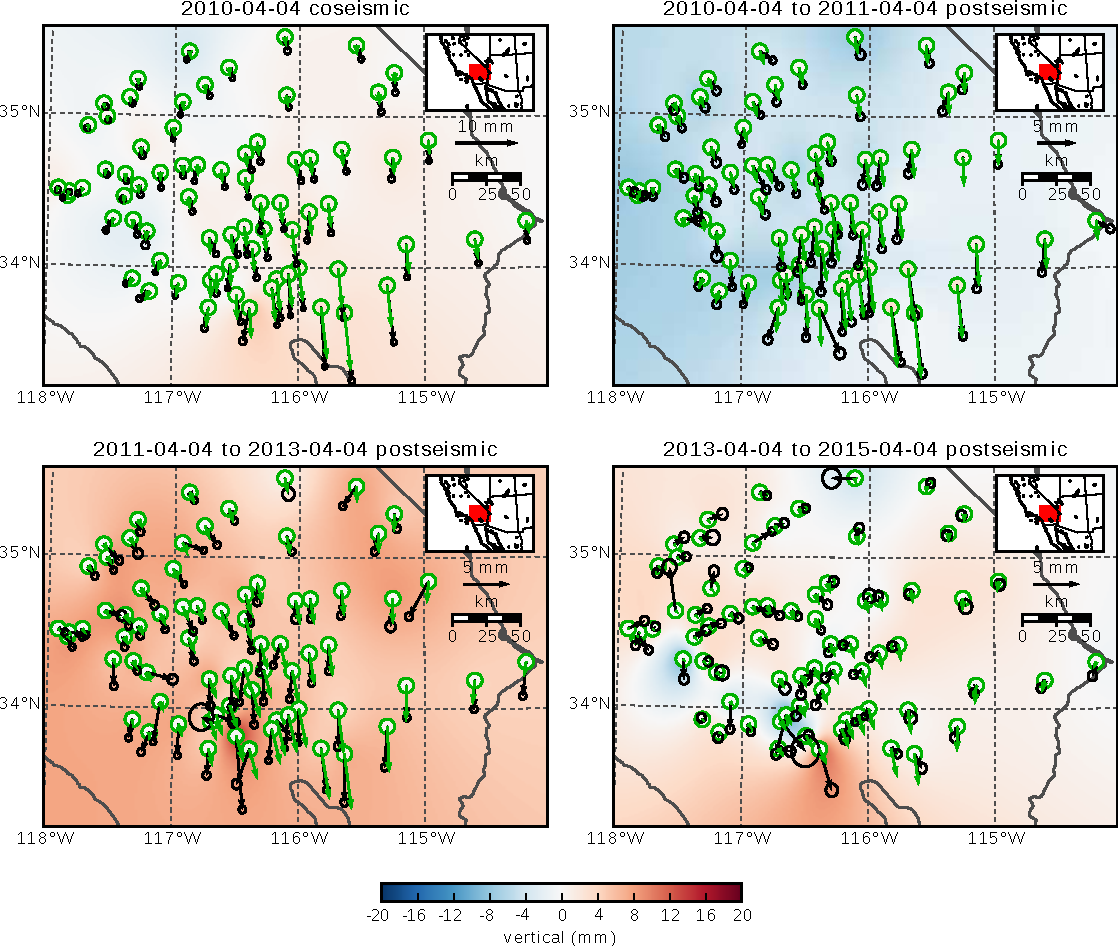
\includegraphics[scale=0.9]{ch3/figures/2016jb013114-p05}
\caption
[Observed and predicted far-field postseismic deformation]
{Same as Figure \ref{ch3:fig:NearField} but for far-field stations.}
\label{ch3:fig:FarField}
\end{figure}

The near-field postseismic deformation is notably sustained when
compared to the far-field deformation.  Namely, the station in this
study which is closest to the El Mayor-Cucapah epicenter, P496, has a
steady postseismic trend of ${\sim}1.5$ cm/yr to the south after about
one year.  Vertical postseismic deformation in the near-field does
display a quadrant pattern which is consistent with the coseismic
vertical deformation, suggesting that it is resulting from postseismic
processes.  However, the vertical postseismic signal is only apparent
for the first year after the earthquake (Figure
\ref{ch3:fig:NearField}).  As with the far-field deformation, there is
a general trend of uplift in the near-field after about one year.

\section{Postseismic modeling}\label{ch3:sec:Model}

\begin{table}\label{ch3:tab:MaterialProperties}
\begin{tabular} {l l l l l}
depth (km) &$\lambda$ (GPa)&$\mu$ (GPa)&$\eta_\mathrm{eff}$ ($10^{18}$ Pa s) & $\mu_\mathrm{k}/\mu$\\ \hline
0-5 & 24.0 & 24.0 & - & -\\
5-15 & 35.0 & 35.0 & - & -\\
15-30 & 42.0 & 42.0 & 44.3 & 0.0\\
30-60 & 61.0 & 61.0 & 5.91 & 0.375\\
60-90 & 61.0 & 61.0 & 1.99 & 0.375\\
90-120 & 61.0 & 61.0 & 1.31 & 0.375\\
120-150 & 61.0 & 61.0 & 1.10 & 0.375\\
150-$\infty$ & 61.0 & 61.0 & 1.07 & 0.375\\
\end{tabular}
\caption
[Assumed and estimated material properties]
{Assumed and estimated material properties. $\lambda$ and
$\mu$ are assumed known \textit{a priori} and are based on the values
used for the coseismic model by \citet{Wei2011}.  The values for
$\eta_\mathrm{eff}$ are estimated in Section
\ref{ch3:sec:InitialInversion}, and $\frac{\mu_k}{\mu}$ are the
optimal shear moduli ratios found in Section
\ref{ch3:sec:FullInversion} for a Zener rheology upper mantle.}
\end{table}

We seek to find the mechanisms driving five years of postseismic
deformation following the El Mayor-Cucapah earthquake and we consider
afterslip and viscoelastic relaxation as candidate mechanisms.
Poroelastic rebound has also been used to model postseismic
deformation \citep[e.g.,][]{Jonsson2003}; however,
\citet{Gonzalez-ortega2014} found that poroelastic rebound is unlikely
to be a significant contributor to postseismic deformation following
the El Mayor-Cucapah earthquake. Furthermore, we consider stations
which are sufficiently far away from the rupture that poroelastic
rebound should be insignificant.

We estimate coseismic and time-dependent postseismic fault slip, both
of which are assumed to occur on a fault geometry modified from
\citet{Wei2011}.  Field studies \citep{Fletcher2014} and LIDAR
observations \citep{Oskin2012} have revealed a significantly more
complicated fault geometry than what was inferred by \citet{Wei2011},
especially within the Sierra Cucapah.  However, we find that a
relatively simple coseismic fault geometry based on \citep{Wei2011} is
adequate because most of the stations used in this study are
sufficiently far from the El Mayor-Cucapah rupture that they are
insensitive to the details in the fault geometry found by
\citet{Fletcher2014} and \citet{Oskin2012}.  The fault geometry used
in this study (Figure \ref{ch3:fig:ContextMap}) consists of the two
main fault segments inferred by \citet{Wei2011}, where the northern
segment runs through the Sierra Cucapah up to the US-Mexico border and
the southern segment is the Indiviso fault which extends down to the
Gulf of California. Both segments extend from the surface to 15 km
depth.  We extend the northern segment by 40 km to the northwest,
which is motivated by the clustering of aftershocks on the northern
tip of the coseismic rupture zone \citep{Hauksson2011,Kroll2013}.
This extended fault segment was also found to be necessary by
\citet{Rollins2015} and \citet{Pollitz2012} in order to describe the
postseismic deformation.

\subsection{Elastic postseismic inversion}\label{ch3:sec:ElasticInversion}    
We consider a variety of rheologic models for the lower crust and
upper mantle. The simplest rheologic model is to consider them to be
effectively elastic and isotropic.  In such case, the rheologic
parameters consist of the reasonably well known Lam\'e parameters,
$\lambda$ and $\mu$, and we use the same values used by
\citet{Wei2011} throughout this paper (Table 1).  The only unknown is
the distribution of fault slip, which can be estimated from
postseismic deformation through linear least squares.
\citet{Rollins2015} used a subset of the GPS stations considered in
this study and found that three years of postseismic deformation
following the El Mayor-Cucapah earthquake can be explained with
afterslip on the coseismic fault plane without requiring any
viscoelastic relaxation. We also perform an elastic slip inversion,
but we use GPS stations within a larger radius about the El
Mayor-Cucapah epicenter (400 km instead of ${\sim}200$ km). Our
forward problem describing predicted postseismic deformation,
$u_\mathrm{pred}$, in terms of time dependent fault slip, $s$, is
\begin{equation}\label{ch3:eq:ElasticForward}
  u_\mathrm{pred}(x,t) = \int_F s(\xi,t)g(x,\xi)d\xi, 
\end{equation}           
where $F$ denotes the fault and $g(x,\xi)$ is the elastic Green's
function describing displacement at surface position $x$ resulting
from slip at $\xi$ on the fault.  We estimate coseismic slip and the
rate of afterslip over the postseismic time intervals 0.0-0.125,
0.125-0.25, 0.25-0.5, 0.5-1.0, 1.0-2.0, 2.0-3.0, 3.0-4.0, and 4.0-5.0
years.  Each fault segment is discretized into roughly 4 km by 4 km
patches an we impose that the direction of slip and slip rate are
within 45$^\circ$ of right-lateral. We also add zeroth-order Tikhonov
regularization so that our solution for $s$ satisfies
\begin{equation}\label{ch3:eq:ElasticObjective}
  \min_s \left(\left|\left|\frac{u_\mathrm{pred}(s) - u_\mathrm{post}}                
                                {\sigma_\mathrm{post}}\right|\right|_2^2 + 
                                \lambda_s||s||_2^2\right),
\end{equation}
where $\sigma_\mathrm{post}$ is the uncertainty on postseismic
displacements and $\lambda_s$ is a penalty parameter which is chosen
with a trade-off curve.  We use Pylith \citep{Aagaard2013} to compute
the Green's functions for this inversion as well as for the remaining
inversions in this paper.

Our coseismic slip and afterslip solutions are shown in Figure
\ref{ch3:fig:ElasticSlip}.  Similar to \citet{Rollins2015}, we find
that a large amount of afterslip on the Indiviso fault segment is
required to explain the observations. The potency of our inferred
coseismic slip is $3.2\times10^9\ \mathrm{m}^3$, equivalent to a
Mw=7.28 earthquake when assuming a shear modulus of 32 GPa.  The
potency of our inferred cumulative five years of afterslip is
$6.1\times10^9\ \mathrm{m}^3$, equivalent to a Mw=7.46 earthquake,
which is unrealistically large if we consider afterslip to be driven
by coseismically induced stresses.  Figure
\ref{ch3:fig:RecordSectionMain} shows the time series for the observed
and predicted postseismic displacements at stations along the El
Mayor-Cucapah P-axis.  We show the radial component of displacements
with respect to the El Mayor-Cucapah epicenter and we also rescale the
displacements so that the difference between the minimum and maximum
observed displacements are the same for each station.  Our elastic
slip model accurately describes near-field postseismic deformation and
systematically underestimates postseismic deformation at epicentral
distances ${\gtrsim}150$ km.  When the fault segments used in the
inversion are extended down to 30 km depth, rather than 15 km, the
systematic far-field residuals are smaller but remain apparent.
Because an elastic model requires an unrealistic amount of afterslip
and is unable to predict far-field deformation, we move on to consider
viscoelastic models in the next section.

\begin{figure}
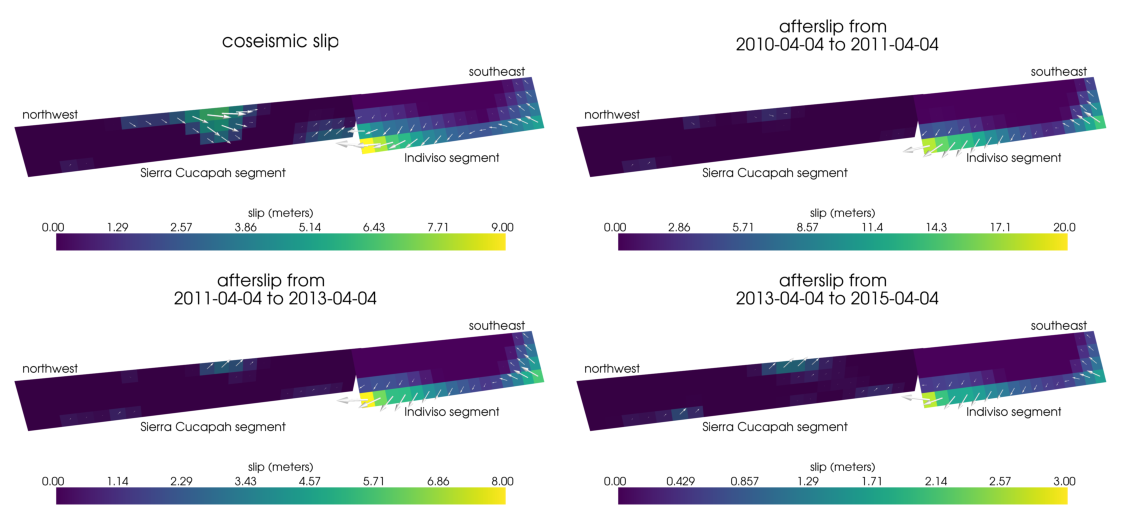
\includegraphics[scale=0.9]{ch3/figures/2016jb013114-p06}
\caption
[Inferred coseismic slip and afterslip when assuming an elastic
lithosphere]
{Coseismic slip and cumulative afterslip over the indicated
time intervals when assuming the crust and mantle are elastic.  Color
indicates the magnitude of slip and arrows indicate the motion of the
hanging wall.}
\label{ch3:fig:ElasticSlip}
\end{figure}

\begin{figure}
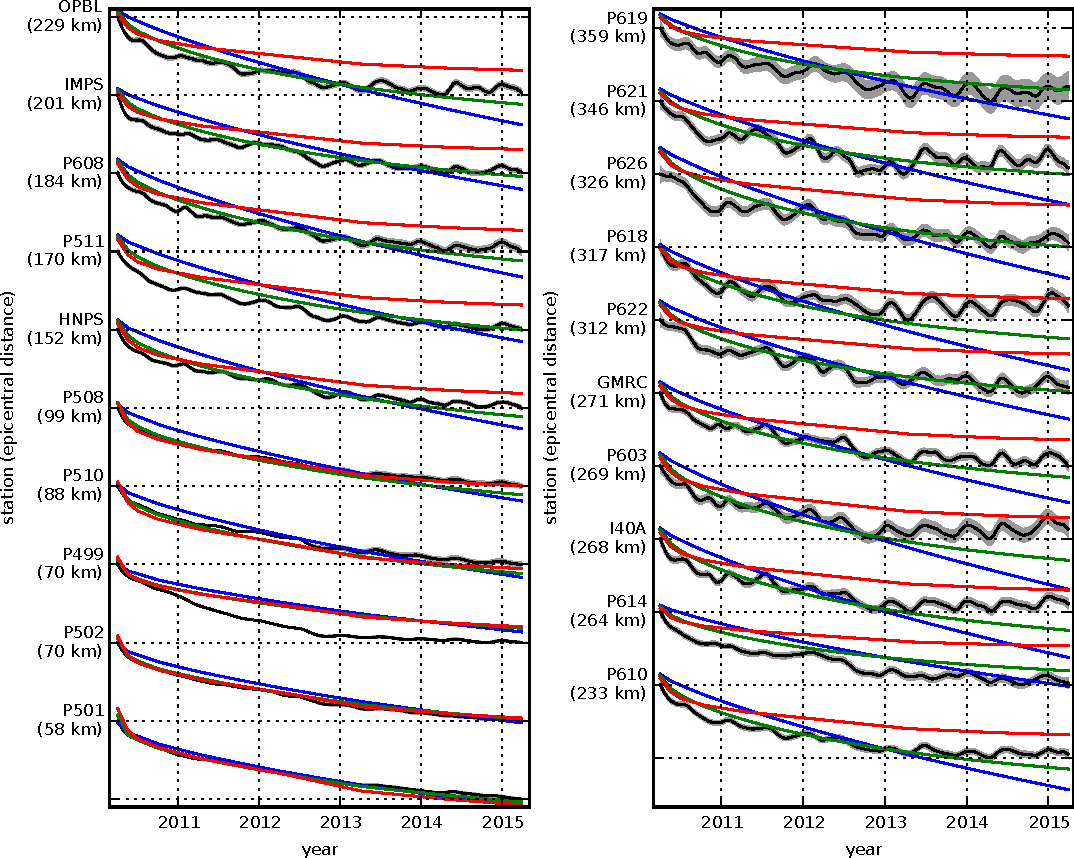
\includegraphics[scale=0.9]{ch3/figures/2016jb013114-p07}
\caption
[Radial components of observed and predicted postseismic displacments]
{Scaled radial component of postseismic displacements.
Downward motion indicates that the station is moving toward the El
Mayor-Cucapah epicenter.  Displacement time series are scaled so that
the minimum and maximum observed values lie on the grid lines.  The
observed postseismic displacements, $u_\mathrm{post}$ are shown in
black with gray indicating the 68\% confidence interval.  The
displacements predicted by the best fitting elastic model are shown in
red.  The blue and green lines are the predicted postseismic
displacements for the models discussed in Section
\ref{ch3:sec:FullInversion}. The blue lines show the predicted
displacements for the model with a Maxwell viscoelastic lower crust
and upper mantle.  The green line shows the predicted displacements
for our preferred model, which has a Maxwell viscoelastic lower crust
and a Zener viscoelastic upper mantle.  The effective viscosities are
the same for both models and are shown in Figure
\ref{ch3:fig:EffectiveViscosity}.}
\label{ch3:fig:RecordSectionMain}
\end{figure}

\subsection{Early postseismic inversion}\label{ch3:sec:InitialInversion}
For any linear viscoelastic rheology of the crust and mantle,
postseismic displacements resulting from time dependent fault slip can
be described as
\begin{equation}\label{GeneralForward}
  u_\mathrm{pred}(x,t) = \int_F s(\xi,t)g(x,\xi)d\xi + 
           \int_0^t\int_F s(\xi,\tau) f(t-\tau,x,\xi) d\xi d\tau,
\end{equation}
where $f(t,x,\xi)$ describes the time-dependent velocity at $x$
resulting from viscoelastic relaxation of stresses induced by slip at
$\xi$. $f$ is a function of $\lambda$, $\mu$, and any additional
rheologic parameters controlling the viscoelastic response, which are
generally not well known. Schematic representations of the
viscoelastic rheologic models considered in this study are shown in
Figure \ref{ch3:fig:Rheology}.  We discuss these rheologic models and
their use in geophysical studies in Section \ref{Discussion}.

\begin{figure}
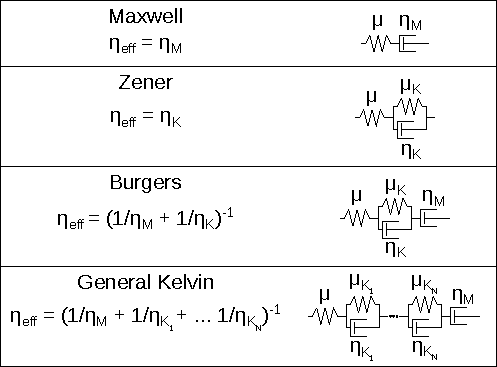
\includegraphics[scale=1.0]{ch3/figures/2016jb013114-f08}
\caption
[Schematic illustration of rheologic models]
{Schematic illustration of the rheologic models considered in
this paper as well as their effective viscosities.}
\label{ch3:fig:Rheology}
\end{figure}

In order to greatly simplify the inverse problem, we use the method
described in \citet{Hines2016} to constrain an initial effective
viscosity structure from the early postseismic deformation.  Our
method uses the fact that coseismic stresses throughout the crust and
upper mantle depend on the instantaneous elastic parameters and are
independent of the viscoelastic parameters which we wish to estimate.
Immediately following an earthquake, each parcel will have a strain
rate that is proportional to the coseismic stress and inversely
proportional to the parcel's effective viscosity, $\eta_\mathrm{eff}$.
Using one-dimensional rheologic models, we define the effective
viscosity as
\begin{equation}
  \eta_\mathrm{eff} = \left.\frac{\sigma}{\dot{\varepsilon}}\right|_{t=0},
\end{equation}
where $\sigma$ is an applied stress at $t=0$ and $\dot\varepsilon$ is
the resulting strain rate.  Figure \ref{ch3:fig:Rheology} shows how
$\eta_\mathrm{eff}$ relates to the parameters for various linear
viscoelastic rheologies.  We can deduce that the initial rate of
surface deformation resulting from viscoelastic relaxation is a
summation of the surface deformation resulting from relaxation in each
parcel, scaled by the reciprocal of the parcel's effective viscosity.
That is to say
\begin{equation}\label{InitialRate}
  f(0,x,\xi) = \int_L \frac{h(x,\xi,\zeta)}{\eta_\mathrm{eff}(\zeta)} d\zeta, 
\end{equation}
where $L$ denotes the crust and mantle and $h(x,\xi,\zeta)$ describes
the initial rate of deformation resulting from viscoelastic relaxation
at $\zeta$ induced by slip at $\xi$. We can combine eq.
(\ref{InitialRate}) with eq. (\ref{GeneralForward}) to get a
first-order approximation for early postseismic deformation,
\begin{equation}\label{ApproxForward}
  u_\mathrm{pred}(x,t) \approx \int_F s(\xi,t)g(x,\xi)d\xi + 
           \int_0^t\int_F\int_L \frac{s(\tau,\xi)}{\eta_\mathrm{eff}(\zeta)} h(x,\xi,\zeta) d\zeta d\xi d\tau,
\end{equation}
which is valid for as long as the rate of deformation resulting from
viscoelastic relaxation is approximately constant.  Although eq.
(\ref{ApproxForward}) may only be valid for a short portion of the
postseismic period, its utility becomes apparent when noting that $g$
and $h$ are only functions of the fault geometry and instantaneous
elastic properties, $\lambda$ and $\mu$, and thus $g$ and $h$ can be
computed numerically as a preprocessing step.  The forward problem in
eq. (\ref{ApproxForward}) can then be rapidly evaluated for any
realization of $s$ and $\eta_{\mathrm{eff}}$.  This is in contrast to
evaluating the full forward problem, eq. (\ref{GeneralForward}),
numerically for each realization of $s$ and the unknown rheologic
properties.

Details on how eq. (\ref{ApproxForward}) is used to estimate $s$ and
$\eta_\mathrm{eff}$ from postseismic deformation can be found in
\citet{Hines2016}.  A non-linear Kalman filter based inverse method
can also be used to estimate $s$ and $\eta_{\mathrm{eff}}$ in a manner
similar to \citet{Segall1997} or \citet{McGuire2003}, in which we
would not have to explicitly impose a time dependent parametrization
of $s$. We have thoroughly explored Kalman filter based approaches,
but we ultimately prefer the method described in \citet{Hines2016}
because of its relative simplicity. Moreover, we believe the piecewise
continuous representation of slip with respect to time is sufficiently
general for the resolving power of these GPS data.

We estimate coseismic slip and afterslip with the same spatial and
temporal discretization as in Section \ref{ch3:sec:ElasticInversion}.
Simultaneously, we estimate $\eta_{\mathrm{eff}}$ within six
vertically stratified layers which have depths ranging from 15-30 km,
30-60 km, 60-90 km, 90-120 km, 120-150 km, and from 150 km to the
bottom of our numerical model domain at 800 km.  We again restrict
fault slip to occur between 0 and 15 km depth, which is done in order
to help eliminate inevitable non-uniqueness in the inversion.  It is
well understood that fault slip at sufficiently great depths can
produce surface deformation that is indistinguishable from
viscoelastic relaxation, at least in two-dimensional earthquake models
\citep{Savage1990}.  Additionally, we note that when simultaneously
estimating both afterslip and viscosity in the lower crust, the
inverse problem becomes particularly ill-posed. This ill-posedness is
illustrated in Figure \ref{ch3:fig:LowerCrust}, which shows the
displacements resulting from a meter of slip on a fault extending from
15 to 30 km depth and the initial velocity resulting from subsequent
viscoelastic relaxation in the lower crust, which is given a viscosity
of $10^{18}$ Pa s.  In this demonstration, the viscoelastic relaxation
is entirely driven by the fault slip in the lower crust.  The
horizontal displacements from fault slip are in the opposite direction
as the displacements resulting from viscoelastic relaxation.  This
means that surface displacements resulting from afterslip at lower
crustal depths can be cancelled out, at least partially, by a low
viscosity lower crust.  We eliminate this null space by allowing only
one mechanism in the lower crust, which we choose to be viscoelastic
relaxation.  This is not to say that we do not believe deep afterslip
is a possibility; rather, we restrict slip to seismogenic depths as a
modeling necessity. Although, it has been noted that the pattern of
vertical postseismic deformation following the El Mayor-Cucpah
earthquake indicates that a significant amount of afterslip must be
shallow \citep{Rollins2015}.
 
\begin{figure}
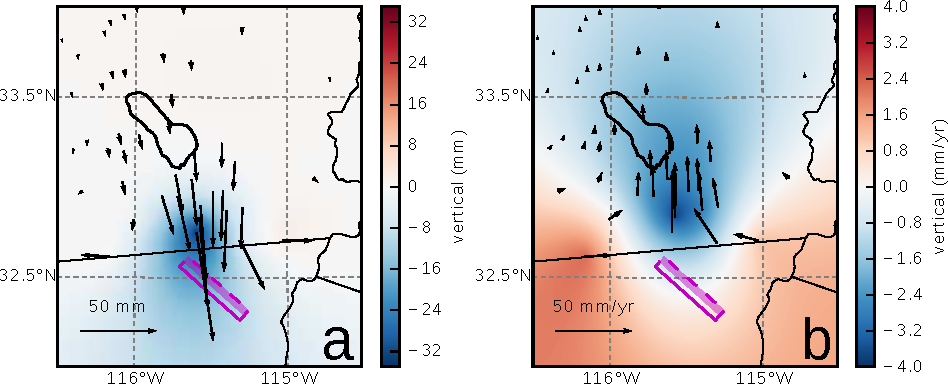
\includegraphics[scale=1.0]{ch3/figures/2016jb013114-p09}
\caption
[Postseismic displacements resulting from deep fault slip and a weak
lower crust]
{Displacements resulting from fault slip at lower crustal
depths (a), and initial velocities resulting from subsequent
relaxation of a viscoelastic lower crust (b).  The fault segment dips
$75^\circ$ to the north-east and its surface projection is outlined in
magenta.  The highlighted area on the fault extends from 15 to 30 km
depth and indicates where 1 meter of right-lateral slip was imposed.
The elastic properties of the crust and mantle are the same as in
Table 1, and $\eta_\mathrm{eff}$ is $10^{18}$ Pa s in the lower crust.
Vertical displacements are interpolated between station locations.}
\label{ch3:fig:LowerCrust} 
\end{figure}
 
We must determine at which point the early postseismic approximation
breaks down, which we will denote as $t_{\mathrm{bd}}$.  As noted, eq.
(\ref{ApproxForward}) is valid for as long as the rate of deformation
resulting from viscoelastic relaxation is approximately constant. We
can almost certainly assume that deformation at the most far-field
stations, which are ${\sim}400$ km away from the El Mayor-Cucapah
epicenter, is the result of viscoelastic relaxation. The approximation
should then be valid for as long as a linear trend adequately
approximates the far-field deformation. Using this logic, it would
appear that $t_{\mathrm{bd}}$ is about one year after the El
Mayor-Cucapah earthquake.  Another way to determine $t_{\mathrm{bd}}$
is to find the best fitting prediction of eq. (\ref{ApproxForward}) to
observed deformation using increasing durations of the postseismic
time series.  $t_\mathrm{bd}$ should be the point when eq.
(\ref{ApproxForward}) is no longer capable of describing the observed
deformation without incurring systematic misfits.  When using eq.
(\ref{ApproxForward}) to fit the entire five years of postseismic
displacements, we see that the near-field displacements (e.g., station
P501) are accurately predicted. When looking at displacements in the
far-field (e.g., station P621), we see that eq. (\ref{ApproxForward})
overestimates the rate of deformation in the later postseismic period
and underestimates the rate of deformation in the early period (Figure
\ref{ch3:fig:RecordSection1}).  Due to the low signal-to-noise ratios
for far-field stations, it is difficult to determine at what point eq.
(\ref{ApproxForward}) is no longer able to predict the observed
displacements; however, we settle on $t_{\mathrm{bd}}=0.8$ years after
the earthquake, while acknowledging that the choice is subjective. As
noted in \citet{Hines2016}, overestimating $t_{\mathrm{bd}}$ will
result in a bias towards overestimating $\eta_{\mathrm{eff}}$, while
picking a $t_\mathrm{bd}$ which is too low will not necessarily result
in a biased estimate of $\eta_\mathrm{eff}$, although the
uncertainties would be larger. We can then consider inferences of
$\eta_{\mathrm{eff}}$ to be an upper bound on the viscosity needed to
describe the far-field rate of deformation during the first 0.8 years
of postseismic deformation.

\begin{figure}
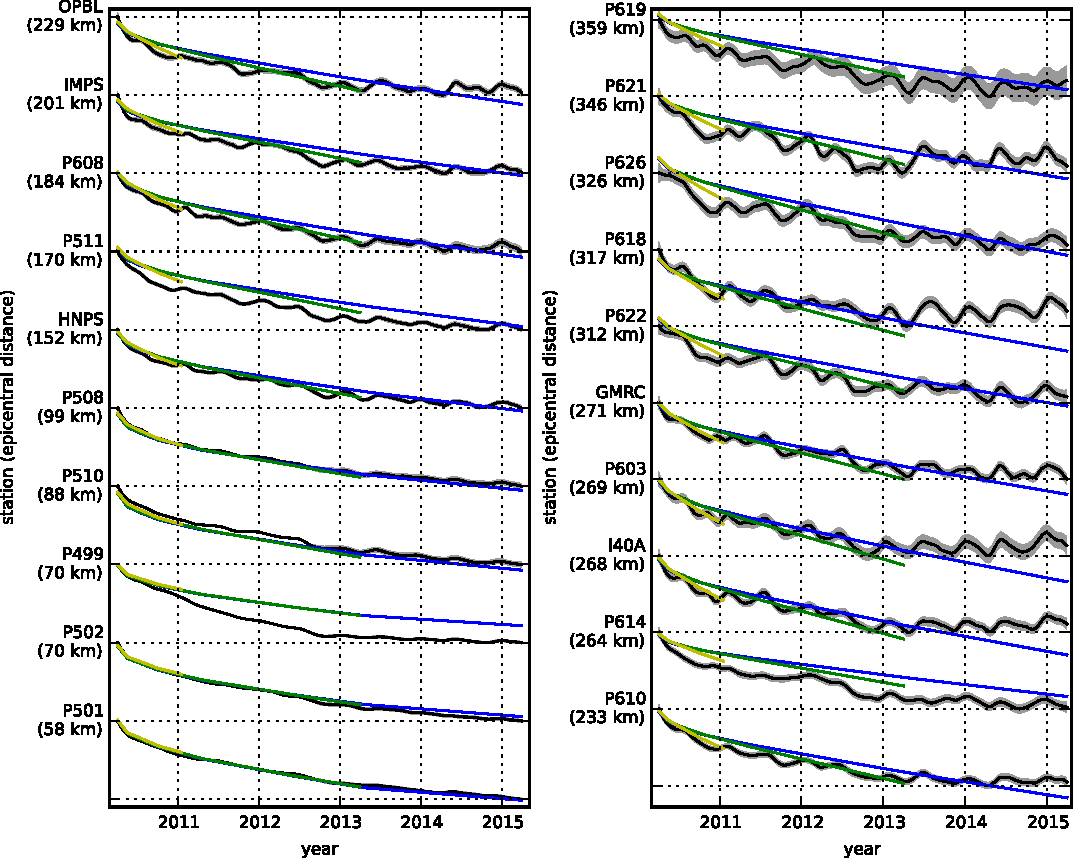
\includegraphics[scale=0.9]{ch3/figures/2016jb013114-p10}
\caption
[Observed postseismic displacments and predicted postseismic
displacments when using varying durations of the data]
{Observed postseismic displacements (black) and best fitting
predictions of eq. (\ref{ApproxForward}) to 5.0 (blue), 3.0 (green),
and 0.8 (yellow) years of the postseismic data.}
\label{ch3:fig:RecordSection1}
\end{figure}

We estimate coseismic slip, afterslip, and effective viscosities by
solving
\begin{equation}\label{ObjectiveFunction}
 \mathrm{min}_{s,\eta_\mathrm{eff}} \left(\left|\left|
 \frac{u_\mathrm{pred}(s,\eta_\mathrm{eff}) - u_\mathrm{post}}
 {\mathbf{\sigma_\mathrm{post}}}\right|\right|_2^2 + 
 \lambda_s||s||_2^2 + 
 \lambda_\eta||\nabla \eta_{\mathrm{eff}}^{-1}||_2^2\right),
\end{equation} 
where $u_\mathrm{post}$ consists of the first 0.8 years of postseismic
deformation and $u_\mathrm{pred}$ are the predicted displacements from
eq. (\ref{ApproxForward}).  Due to inherent non-uniqueness, we have
added zeroth-order Tikhonov regularization to estimates of $s$ and
second-order Tikhonov regularization to estimates of effective
fluidity $\eta_\mathrm{eff}^{-1}$. The degree to which we impose the
regularization on slip and fluidity is controlled by the penalty
parameters $\lambda_s$ and $\lambda_\eta$, which are chosen with
trade-off curves (Figure \ref{ch3:fig:S1}).  Our goal is to get a prior constraint
on $\eta_{\mathrm{eff}}$ to minimize the amount of searching we have
to do when describing the postseismic deformation over the full five
years, which we do in Section \ref{ch3:sec:FullInversion}.  Estimates
of $s$ made here will not be used in Section
\ref{ch3:sec:FullInversion}, and so the motivation behind adding
regularization to $s$ is to ensure that the slip driving viscoelastic
relaxation in eq. (\ref{ApproxForward}) is sensible.

Our initial estimate for coseismic slip and cumulative afterslip over
the first 0.8 years after the El Mayor-Cucapah earthquake are shown in
Figure \ref{ch3:fig:InitialSlip}.  Similar to our elastic slip model
from Section \ref{ch3:sec:ElasticInversion}, a significant amount of
right-lateral and normal coseismic slip is inferred to be on the
Sierra Cucapah segment. Our coseismic slip solution on the Sierra
Cucapah segment is consistent with field studies \citep{Fletcher2014}
and the model from \citet{Wei2011}.  Our inferred slip on the Indiviso
fault segment differs from \citet{Wei2011} because the GPS data used
in this study is not capable of resolving the spatial distribution of
fault slip on that segment (Figure \ref{ch3:fig:S2}).  The potency of inferred
coseismic slip is $3.3\times 10^{9}\ \mathrm{m}^3$, which is also
about the same as that inferred from Section
\ref{ch3:sec:ElasticInversion}. The present inference of afterslip on
the Indiviso fault is significantly less than what was found in the
Section \ref{ch3:sec:ElasticInversion} where we did not account for
viscoelasticity. When fault slip is simultaneously estimated with
viscosity, the potency of inferred afterslip over the first 0.8 years
after the earthquake is $0.85\times 10^9\ \mathrm{m}^3$, compared to
$3.5\times10^{9}\ \mathrm{m}^3$ when we assume the crust and upper
mantle are elastic.  The significant amount of afterslip inferred on
the Indiviso fault in Section \ref{ch3:sec:ElasticInversion} seems to
be compensating for unmodeled viscoelastic relaxation.  The fact that
there is still an appreciable amount of afterslip inferred on the
Indiviso fault raises the question of whether it is compensating for
viscoelastic relaxation that is more localized than what we allow for
since we only estimate depth dependent variations in viscosity.

Our estimated effective viscosities, and corresponding fluidities, are
shown in Figure \ref{ch3:fig:EffectiveViscosity}.  Although fluidity
is rarely used in geophysical literature, eq. (\ref{InitialRate}) is
linear with respect to fluidity and so the fluidity indicates the
amplitude of the viscoelastic signal coming from each layer.  We use
bootstrapping to find the 95\% confidence intervals for our estimated
effective viscosities which are shown as shaded regions in Figure
\ref{ch3:fig:EffectiveViscosity}.  It is important to remember that
the presented effective viscosities were estimated with a smoothing
regularization constraint and so the uncertainties are almost
certainly underestimated \citep{Aster2011}.  Indeed, many viscosity
profiles which are outside of the shown confidence intervals can just
as adequately described the first 0.8 years of postseismic
deformation. Our solution in Figure \ref{ch3:fig:EffectiveViscosity}
should be interpreted as the smoothest effective viscosity profile
which is capable of describing the data.  This means that any sharp
viscosity transitions will be tapered out in the inversion, which we
demonstrate with a synthetic test in Figure \ref{ch3:fig:S2}.  Nonetheless, a robust
feature that we see with a variety of choices for $\lambda_s$,
$\lambda_\eta$, and $t_\mathrm{bd}$ is that the largest jump in
fluidity is at 60 km depth, which is consistent with the range of
lithosphere-asthenosphere boundary depths inferred by
\citet{Lekic2011}. This transitional depth is also consistent with the
the viscosity structure required to explain far-field postseismic
deformation following the Hector Mine earthquake \citep{Freed2007a}.
We find that the viscosity below 60 km depth needs to be
${\sim}1\times10^{18}$ Pa s to describe the early rate of postseismic
deformation at far-field stations while the lower crust and uppermost
mantle need to be relatively stronger.  The viscosity of the lower
crust has the largest uncertainties because there is no evidence of
relaxation in that layer, meaning that it is effectively elastic over
the first 0.8 years after the earthquake.

\begin{figure}
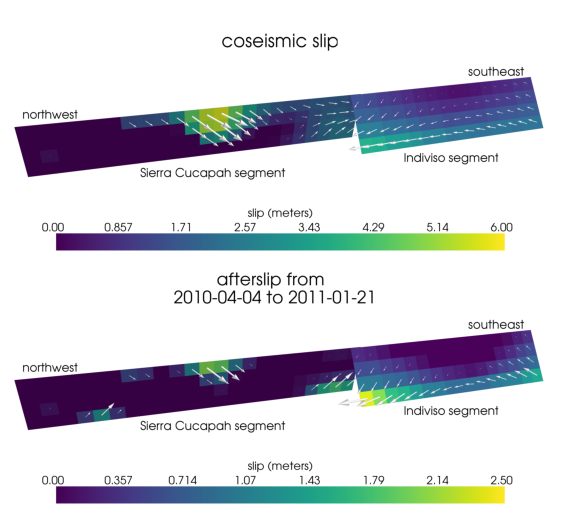
\includegraphics[scale=1.0]{ch3/figures/2016jb013114-p11}
\caption
[Coseismic slip and afterslip inferred from 0.8 years of postseismic
data]
{Coseismic slip and afterslip inferred by fitting eq.
(\ref{ApproxForward}) to the first 0.8 years of postseismic
displacements.}
\label{ch3:fig:InitialSlip}
\end{figure} 

\begin{figure}
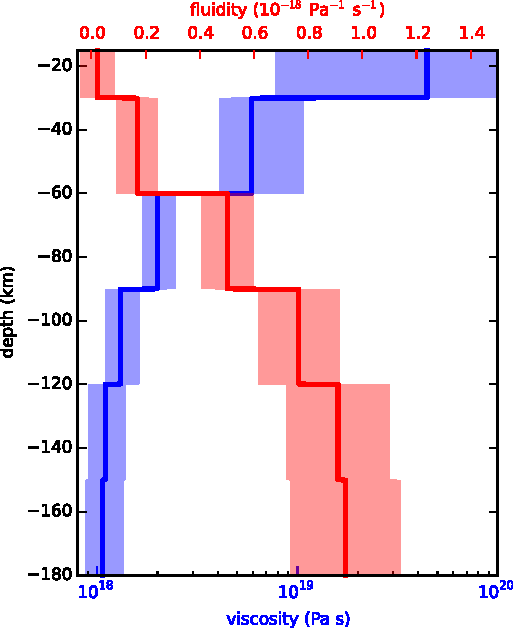
\includegraphics[scale=1.0]{ch3/figures/2016jb013114-p12}
\caption
[Inferred effective viscosities]
{Effective viscosities and associated fluidities inferred by
fitting eq. (\ref{ApproxForward}) to the first 0.8 years of
postseismic displacements. 95\% confidence intervals, estimated from
bootstrapping, are indicated by shaded regions.}
\label{ch3:fig:EffectiveViscosity}
\end{figure} 

\subsection{Full postseismic inversion}\label{ch3:sec:FullInversion} 
In the previous section, we used the inverse method from
\citet{Hines2016} to constrain the effective viscosity structure
required to explain the first 0.8 years of postseismic deformation. In
this section, we use these effective viscosities as a prior constraint
when searching for models which are capable of describing the
available five years of postseismic data, where our forward problem is
now eq. (\ref{GeneralForward}) rather than the approximation given by
eq. (\ref{ApproxForward}).  We perform a series of fault slip
inversions assuming a variety of rheologies for the lower crust and
upper mantle which are consistent with our findings from Section
\ref{ch3:sec:InitialInversion}.  We appraise each model using the mean
chi-squared value,
\begin{equation}\label{ch3:eq:Misfit}
  \bar\chi^2 = \frac{1}{N}\left|\left|\frac{u_\mathrm{pred} - u_\mathrm{post}}{\sigma_\mathrm{post}}\right|\right|_2^2,
\end{equation}
where $N$ is the number of observations.

We first assume that the crust and mantle can be described with a
Maxwell rheology, and we set the steady-state viscosity,
$\eta_\mathrm{M}$, equal to our inference of $\eta_{\mathrm{eff}}$.
We compute $f$ and $g$ from eq. (\ref{GeneralForward}) using Pylith,
and we use the same spatial and temporal discretization of $s$ as in
Sections \ref{ch3:sec:ElasticInversion} and
\ref{ch3:sec:InitialInversion}. We estimate $s$ using linear least
squares and find a misfit of $\bar\chi^2=37.4$. For comparison,
$\bar\chi^2=35.3$ for the elastic model from Section
\ref{ch3:sec:ElasticInversion}.  The Maxwell viscoelastic model has a
larger misfit because it tends to overestimate the rate of deformation
after about three years (Figure \ref{ch3:fig:RecordSectionMain}).
Since our initial estimates of $\eta_\mathrm{eff}$ may be biased
towards overestimating viscosities, we have also performed the slip
inversion where we use uniformly lower viscosities in the crust and
mantle; however, decreasing the viscosity only increases the misfit.
Although, the viscosities used here are consistent with the successful
Maxwell viscoelastic models found by \citet{Rollins2015} and
\citet{Spinler2015}, which had mantle viscosities on the order of
$10^{18}$ Pa s and relatively higher lower crustal viscosities, we
find that such a model is incapable of describing the entire
postseismic time series.  \citet{Pollitz2001} similarly recognized
this deficiency in a Maxwell rheology, which then motivated their
exploration of a Burgers rheology upper mantle \citep{Pollitz2003}.

Instead of exploring a Burgers rheology mantle, which introduces two
new parameters that need to be estimated, the transient viscosity,
$\eta_{K}$, and transient shear modulus, $\mu_{K}$, we first consider
a Zener rheology for the mantle, which only introduces one unknown
model parameter, $\mu_{K}$.  We assume that the lower crust still has
a Maxwell rheology. The steady-state viscosity in the crust and the
transient viscosity in the mantle are set equal to the inferred
effective viscosities.  We then estimate the ratio of shear moduli,
$\frac{\mu_K}{\mu}$. We compute nine different sets of Green's
functions, $f$ and $g$, where we assume values of $\frac{\mu_K}{\mu}$
ranging from 0 to 1. The former being a degenerate case where the
Zener model reduces to the above Maxwell model.  We estimate coseismic
slip and afterslip for each realization of $\frac{\mu_K}{\mu}$.  We
find that a shear moduli ratio of 0.375 yields the best prediction to
the observed postseismic displacements with a misfit of
$\bar\chi^2=31.2$ (Figure \ref{ch3:fig:ShearModulusRatio}).  The
improvement in the Zener model over the Maxwell model can be seen in
the fit to the far-field data (Figure \ref{ch3:fig:RecordSectionMain})
where the Zener model does a significantly better job at explaining
the transient rate of deformation throughout the five years considered
in this study.  The rheologic parameters for our preferred Zener model
are summarized in Table 1.

\begin{figure}
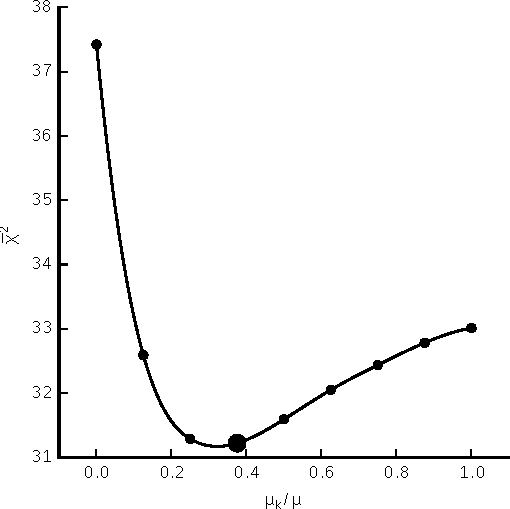
\includegraphics[scale=1.0]{ch3/figures/2016jb013114-f13}
\caption
[Misfit as a function of transient shear modulus]
{Mean chi-squared value as a function of the transient shear
modulus relative to the elastic shear modulus in a Zener rheology
upper mantle. Large dot indicates our preferred ratio.}
\label{ch3:fig:ShearModulusRatio}
\end{figure}

Because we are able to adequately describe the available five years of
postseismic deformation with a Zener model, we do not find it
necessary to explore the parameter space for a more complicated
Burgers rheology.  However, since the Zener model is a Burgers model
with an infinite steady-state viscosity, we can conclude that any
Burgers rheology that has a transient viscosity consistent with that
found in Section \ref{ch3:sec:InitialInversion} and a steady-state
viscosity $\gtrsim10^{20}$ Pa s, which is effectively infinite on the
time scale of five years, would also be able to satisfactorily
describe the observable postseismic deformation.
  
The regularized inference of coseismic slip and afterslip for our
preferred Zener model is shown in Figure \ref{ch3:fig:FinalSlip}.  The
inferred coseismic potency is $3.0\times10^{9}\ \mathrm{m}^3$,
equivalent to a Mw=7.26 earthquake, where most of the slip is shallow
and on the Sierra Cucapah fault segment.  The potency of five years of
afterslip is $1.1\times10^{9}\ \mathrm{m}^3$. Most of the afterslip in
our preferred model occurs within the first year after the earthquake
and coincides with the location of our inferred coseismic slip.
Inferred afterslip within the first year is accounting for the most
rapid near-field transient deformation (Figure \ref{ch3:fig:S3}).  After one year,
afterslip is inferred to be deeper down on the Sierra Cucapah segment.
The sustained near-field postseismic deformation is being explained by
this continued afterslip as well as viscoelastic relaxation in the
lower crust. We emphasize, that the GPS station closest to where we
infer afterslip, P496, is still about 30 km away, which is too far for
us to conclusively discern deep afterslip from viscoelastic relaxation
in the lower crust.  The deep afterslip inferred after one year could
potentially be compensating for an overestimated lower crustal
viscosity.  To test this, we have modified our preferred model by
decreasing the lower crustal viscosity from $4.4\times10^{19}$ Pa s
to $1\times10^{19}$ Pa s, which is still consistent with our viscosity
inference from Section \ref{ch3:sec:InitialInversion}, and we inverted
for fault slip.  We find that a model with a weaker lower crust
adequately describes the postseismic displacements without any
afterslip after one year, while still requiring about the same amount
of afterslip over the first year. We do believe that the early
afterslip on the Sierra Cucapah segment is a robust feature in our
preferred model, while we are not confident in our inference of later
deep afterslip.

The postseismic displacements predicted by our preferred Zener model
are shown in Figures \ref{ch3:fig:NearField}, \ref{ch3:fig:FarField}
and \ref{ch3:fig:RecordSectionMain}.  The largest misfit occur within
the Imperial Valley where there does not appear to be any systematic
trend in the residuals.  This suggests that the large errors are due
to localized processes such as fault slip in the Imperial Valley
triggered by the El Mayor-Cucapah earthquake \citep{Wei2011a,Wei2015}.
We do not see any pattern in the residuals that would suggest a
laterally heterogeneous viscosity structure, which has been explored
by \citet{Pollitz2012} and \citet{Rollins2015}.  We do notice regional
scale seasonal oscillations in the lateral and vertical components of
the residuals with an amplitude of 1-2 millimeters.  This is the
result of our method for data processing which is not able to
completely remove the seasonal signal in the GPS data, which was
discussed in Section \ref{ch3:sec:Data}.  Additionally, we see
systematic misfit in the later postseismic period west of the Landers
and Hector Mine earthquakes, which may be the result of unmodeled
postseismic deformation following those earthquakes.  Lastly, there
are clear discrepancies between the observed and predicted vertical
displacements following the first year after the El Mayor-Cucapah
earthquake. We observe a broad uplift throughout Southern California
which is inconsistent with any postseismic model.

\begin{figure}
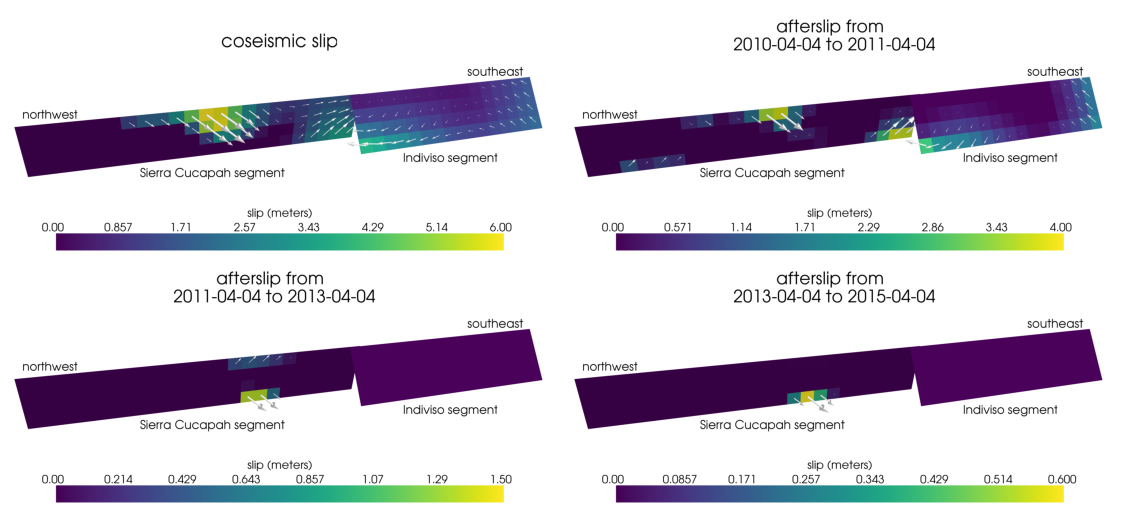
\includegraphics[scale=0.9]{ch3/figures/2016jb013114-p14}
\caption
[Coseismic slip and afterslip inferred from all available postseismic
data]
{Inferred coseismic slip and afterslip for our preferred
model, which has a Maxwell rheology in the lower crust and a Zener
rheology in the upper mantle.  The transient viscosity, $\eta_K$, in
the mantle and steady-state viscosity, $\eta_M$, in the crust are set
equal to the effective viscosities from Figure
\ref{ch3:fig:EffectiveViscosity}. We use $\frac{\mu_K}{\mu}=0.375$ in
the upper mantle.}
\label{ch3:fig:FinalSlip}
\end{figure}
  
\section{Discussion}\label{Discussion}
It has long been recognized that deep afterslip and viscoelastic
relaxation following an upper crustal earthquake can result in similar
horizontal ground deformation at the surface
\citep[e.g.,][]{Savage1990, Pollitz2001, Hearn2003, Feigl2006}. The
similarity of the horizontal postseismic deformation results in a
non-uniqueness in inferences of afterslip or viscoelastic relaxation.
The spatial pattern of vertical postseismic deformation has been
proposed to be a discriminant between deep afterslip and viscoelastic
relaxation \citep[e.g.,][]{Pollitz2001, Hearn2003}. It is, however,
important to note that patterns of vertical deformation are very
sensitive to the depth-dependence of viscosity below the upper crust
\citep{Yang1981,Hetland2014}.  The similarity between deformation
resulting from deep afterslip and viscoelastic relaxation of coseismic
stresses is different from the ill-posedness described in Section
\ref{ch3:sec:InitialInversion}. In our method, any inferred afterslip
will also mechanically drive additional viscoelastic relaxation.  The
horizontal deformation resulting from deep afterslip will generally be
in the opposite direction as horizontal deformation resulting from
viscoelastic relaxation of subsequent stresses in the lower crust
(Figure \ref{ch3:fig:LowerCrust}).  As a result, there is a trade-off
between inferences of deep afterslip and lower crustal viscosity.  In
our synthetic tests in \citet{Hines2016}, we have found that inverting
surface deformation for afterslip and viscosity within the same depth
interval tends to result in overestimated afterslip and an
underestimated viscosity.

Most postseismic studies assume Maxwell viscoelasticity in the lower
crust and upper mantle \citep[e.g.,][]{Nur1974, Pollitz2000,
Hetland2003, Freed2006a, Johnson2009, Hearn2009}, which is the
simplest viscoelastic rheologic model.  In Southern California,
postseismic studies following the Landers \citep{Pollitz2000}, Hector
Mine \citep{Pollitz2001}, and El Mayor-Cucapah earthquake
\citep{Spinler2015,Rollins2015}, have assumed Maxwell viscoelasticity
in the lower crust and upper mantle and have inferred upper mantle
viscosities on the order of $10^{17}$ to $10^{18}$ Pa s and lower
crust viscosities $\gtrsim 10^{19}$ Pa s. These postseismic studies
are consistent with \citet{Kaufmann2000} and \citet{Cavalie2007}, who
found that an upper mantle viscosity of $10^{18}$ Pa s and a crustal
viscosity $\gtrsim10^{20}$ Pa s are necessary to describe subsidence
resulting from changes in loading from Lake Mead. This isostatic
adjustment is a process with similar spatial and temporal scales as
postseismic deformation, and thus the inferred viscosities of these
two types of studies would likely agree. While these studies found
viscosities that are consistent with our effective viscosities from
Section \ref{ch3:sec:InitialInversion}, they are inconsistent with
viscosity estimates made from geophysical processes that occur over
longer time scales. For example, \citet{Lundgren2009} found that lower
crust and upper mantle viscosities on the order of $10^{21}$ and
$10^{19}$ Pa s, respectively, are needed to describe interseismic
deformation along the Southern San Andreas fault zone in the Salton
Sea region.  An even higher mantle viscosity, on the order of
$10^{20}$ Pa s, is required to describe isostatic adjustment resulting
from the draining of Lake Bonneville, which occurs on the time scales
of $10^{4}$ years \citep{Crittenden1967, Bills1987}.

An additional deficiency with the Maxwell rheology is that it predicts
a steady decay in the rate of postseismic deformation over time, which
fails to describe the commonly observed rapid, early transience
followed by a relatively steady rate of postseismic deformation.  One
could explain the early transient postseismic deformation with fault
creep and the later phase with relaxation in a Maxwell viscoelastic
lower crust and upper mantle \citep[e.g][]{Hearn2009,Johnson2009}.
However, postseismic deformation at distances greater than ${\sim}200$
km from the El Mayor-Cucapah epicenter can only be attributed to
viscoelastic relaxation \citep[e.g.,][]{Freed2007a} and we have
demonstrated that the far-field deformation cannot be explained with a
Maxwell rheology (Figure \ref{ch3:fig:RecordSectionMain}).

We found that a Zener rheology in the upper mantle with a transient
viscosity of ${\sim}10^{18}$ Pa s does a noticeably better job at
predicting far-field postseismic deformation.  A generalization of the
Zener viscoelastic model, schematically represented as several Kelvin
elements connected in series, is commonly used to describe seismic
attenuation \citep{Liu1976}.  The highest viscosity needed to describe
seismic attenuation is on the order of $10^{16}$ Pa s \citep{Yuen1982}
which has a characteristic relaxation time on the order of days. Even
though our inferred transient viscosity is orders of magnitude larger
than that required for seismic attenuation models, the two models are
not incompatible.  Rather, the delayed elasticity in seismic
attenuation models occurs on such short time scales that it can be
considered part of the instantaneous elastic phase of deformation
associated with the preferred Zener model in this study.

Of course, a Zener rheology provides an incomplete description of the
asthenosphere because it does not have the fluid-like behavior
required to explain isostatic rebound or convection in the mantle
\citep{OConnell1971}.  \citet{Yuen1982} proposed a Burgers rheology
with a low transient viscosity ($\eta_K\approx10^{16}$ Pa s) and high
steady-state viscosity ($\eta_M\approx10^{21}$ Pa s) to describe both
seismic attenuation and long term geologic processes.  The
justification of a Burger's rheology mantle is further supported by
laboratory experiments on olivine \citep{Chopra1997}.
\citet{Pollitz2003} sought to describe postseismic deformation
following Hector Mine with a Burgers rheology mantle and they found a
best fitting transient viscosity of $1.6\times10^{17}$ Pa s and
steady-state viscosity of $4.6\times10^{18}$ Pa s. While the Burgers
rheology was introduced as a means of bridging the gap between
relaxation observed in long and short term geophysical processes, the
inferred steady state viscosity from \citet{Pollitz2003} is still
inconsistent with the Maxwell viscosities inferred from studies on the
earthquake cycle and Lake Bonneville.  The transient viscosity
inferred by \citet{Pollitz2003} is constrained by the earliest phase
of postseismic deformation following the Hector Mine earthquake. While
\citet{Pollitz2003} ruled out deep afterslip as an alternative
mechanism based on inconsistent vertical deformation, it is still
possible to successfully describe all components of early postseismic
deformation following the Hector Mine earthquake with afterslip at
seismogenic depths \citep{Jacobs2002}. It is then possible that the
preferred rheologic model from \citet{Pollitz2003} was biased towards
inferring a particularly low transient viscosity by neglecting to
account for afterslip.  This is in contrast to the present study,
where we have inferred a viscosity structure simultaneously with
afterslip.  We also argue that a transient rheology is necessary to
explain postseismic deformation; however, our preferred transient
viscosity of ${\sim}10^{18}$ Pa s in the upper mantle is an order of
magnitude larger than the transient viscosity found by
\citet{Pollitz2003}.  The transient viscosity inferred here is
consistent with the results of \citet{Pollitz2015}, who reanalyzed
postseismic data following the Landers and Hector Mine earthquake
allowing the first few months of transient deformation to be described
by afterslip.  Since a Zener model is able to describe the available
postseismic deformation following the El Mayor-Cucapah earthquake, any
Burgers rheology with a steady-state viscosity that is
$\gtrsim10^{20}$ Pa s, effectively infinite over five years, would
also be able to describe the postseismic deformation. Such a Burgers
model might then be consistent with the steady-state viscosities
necessary for lake loading, interseismic deformation, and mantle
dynamics.

\section{Conclusion}
We have extracted a smoothed estimate of postseismic deformation
following the El Mayor-Cucapah earthquake from GPS displacement time
series.  Our estimated postseismic deformation reveals far-field
(epicentral distances ${\gtrsim}200$ km) transient deformation which
is undetectable after about three years. Near-field deformation
exhibits transience that decays to a sustained, elevated rate after
about one or two years.  We found that near-field transient
deformation can be explained with shallow afterslip.  The sustained
rate of near-field deformation can be explained with viscoelastic
relaxation in the lower crust and possibly continued afterslip.
Far-field transient deformation can be more definitively ascribed to
viscoelastic relaxation at depths greater than ${\sim}60$ km. Beneath
that depth, a transient viscosity of ${\sim}1\times10^{18}$ Pa s is
required to describe the rate of far-field deformation throughout the
five years considered in this study.  By describing the available
postseismic deformation with a transient rheology in the mantle, our
preferred model does not conflict with the generally higher
steady-state viscosities inferred from geophysical processes occurring
over longer time scales.

\section{Acknowledgements}
We thank Andy Freed for an illuminating discussion on the data used in
this study.  We thank Fred Pollitz and an anonymous reviewer for
comments that improved this manuscript. We also thank the editor,
Martha Savage.  This material is based on EarthScope Plate Boundary
Observatory data services provided by UNAVCO through the GAGE Facility
with support from the National Science Foundation (NSF) and National
Aeronautics and Space Administration (NASA) under NSF Cooperative
Agreement No. EAR-1261833.  The data used in this study can be found
at www.unavco.org. This material is based upon work supported by the
National Science Foundation under Grant Numbers EAR 1045372 and EAR
1245263.

%\bibliographystyle{agu04}
%\bibliography{refs}

\section{Supporting information}
Figures \ref{ch3:fig:S1} and \ref{ch3:fig:S2} provide additional
information about the inversion in Section \ref{ch3:sec:Model} of the
main text. Figures \ref{ch3:fig:S3} and \ref{ch3:fig:S4} show the
predicted displacements, which have been decomposed into elastic and
viscoelastic components, for the preferred model from Section
\ref{ch3:sec:FullInversion}.

\begin{figure}
\noindent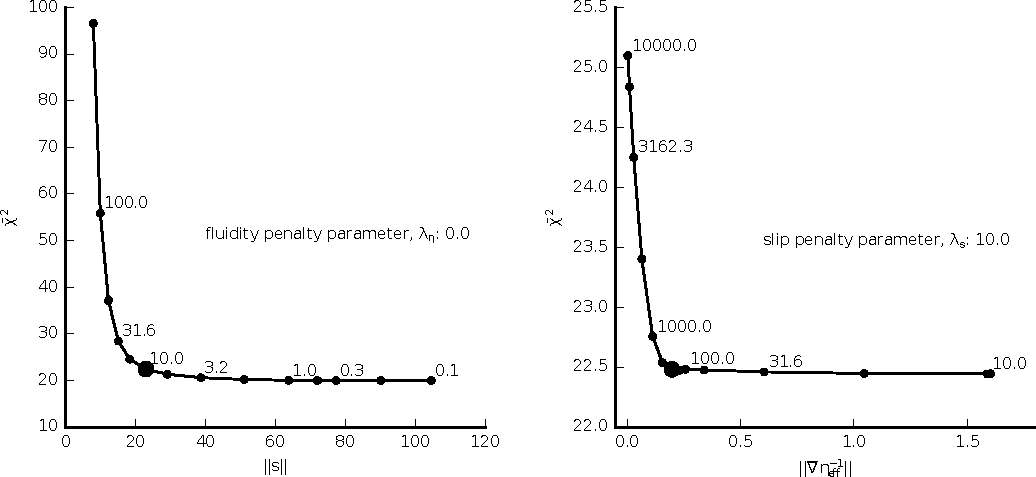
\includegraphics[scale=0.9]{ch3/figures/2016jb013114-fS01}
\caption
[Trade-off curves]
{Trade-off curves used to determine the damping parameters
$\lambda_s$ and $\lambda_\eta$ in eq.  (15) of the main text.  The
left panel shows the trade-off curve for the fault slip penalty
parameter, $\lambda_s$.  We pick $\lambda_s$ while keeping the penalty
parameter for fluidity, $\lambda_\eta$, fixed at zero.  The right
panel shows the trade of curve for selecting $\lambda_\eta$, where we
fix $\lambda_s$ at the chosen value from the left panel. Chosen values
are indicated with the larger marker.  When picking $\lambda_s$, we
try to find a good balance between the mean chi-squared value,
$\bar{\chi}^2$, and the size of the slip parameters, $||s||$.  Our
choice of $\lambda_\eta$ is a balance between $\bar{\chi}^2$ and the
size of the Laplacian of fluidity, $||\nabla
\eta_\mathrm{eff}^{-1}||$.}
\label{ch3:fig:S1}
\end{figure}

\begin{figure}
\noindent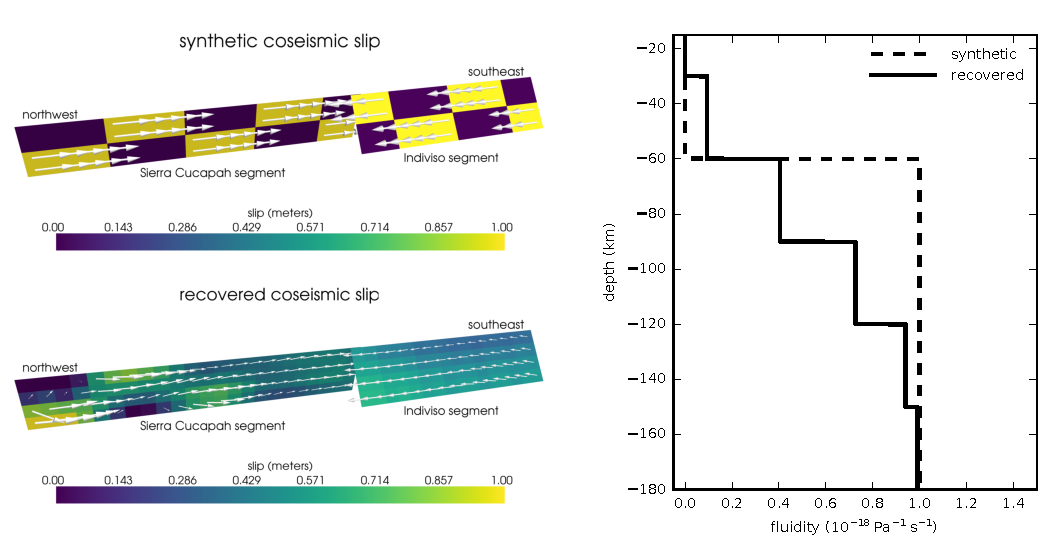
\includegraphics[scale=0.9]{ch3/figures/2016jb013114-pS02}
\caption
[Synthetic checkerboard test]
{Checkerboard test used to assess the resolving power of the
inversion in Section \ref{ch3:sec:InitialInversion} of the main text.  We create synthetic data
at all of the GPS stations considered in this study by evaluating eq.
(14) with the synthetic coseismic slip distribution and fluidity
distributions. Our synthetic fluidity model has a jump from 0.0 to
$10^{-18}$ Pa$^{-1}$ s$^{-1}$ at 60 km depth.  Our synthetic slip
model does not include afterslip, although we estimate afterslip along
with coseismic slip and fluidity in this test.  We estimate these
values in the same way as described in the main text and we also use
the same penalty parameters.  We do not add any noise to our synthetic
data so that the recovered model just indicates how much the
regularization influences the solution.  Note that our ability to
recover slip decreases towards the southern end of the fault, farthest
from the available data.  Also note that the smoothing constraint on
fluidity largely obscures the jump in the synthetic model.}
\label{ch3:fig:S2}
\end{figure}

\begin{figure}
\noindent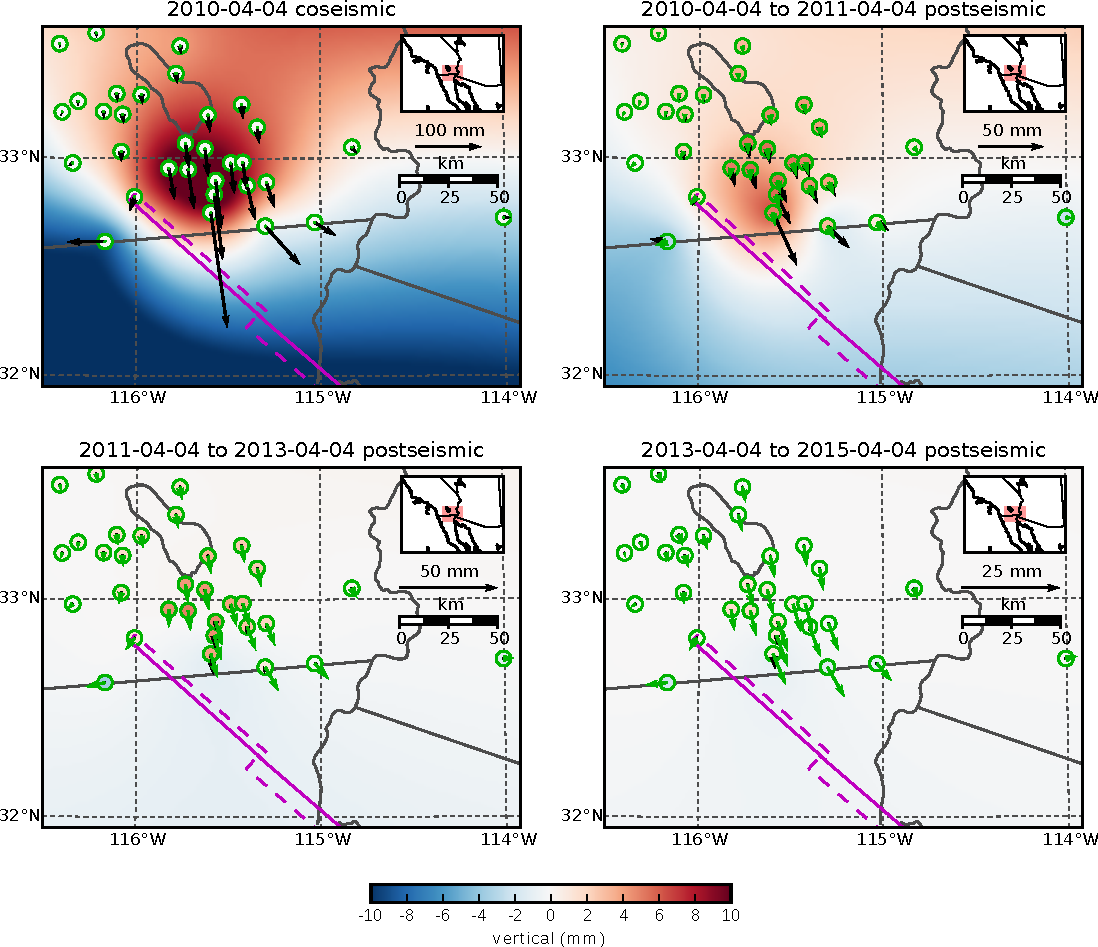
\includegraphics[scale=0.9]{ch3/figures/2016jb013114-pS03}
\caption
[Elastic and viscous components of predicted near-field postseismic
displacments]
{Elastic (black) and viscoelastic (green) components of the
near-field predicted displacements for the preferred Zener model from
Section \ref{ch3:sec:FullInversion}.  The elastic component is the deformation resulting from
fault slip and the viscoelastic component is the deformation resulting
from viscoelastic relaxation of stresses induced by the fault slip.
The elastic and viscoelastic components are calculated from the first
and second terms in eq. (11), respectively.  The vertical elastic
component is shown as an interpolated field and the vertical
viscoelastic component is shown within the green circles.}
\label{ch3:fig:S3}
\end{figure}

\begin{figure}
\noindent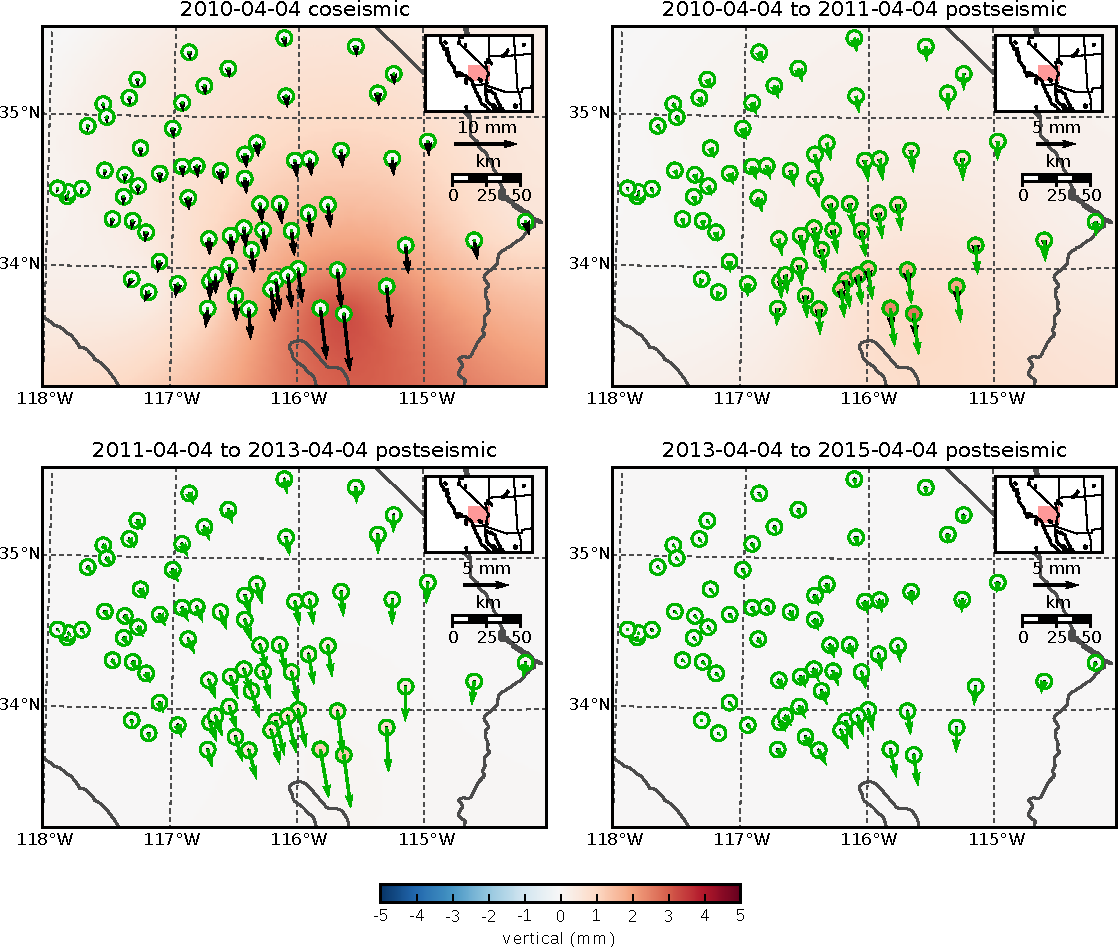
\includegraphics[scale=0.9]{ch3/figures/2016jb013114-pS04}
\caption
[Elastic and viscous components of predicted far-field postseismic
displacments]
{Same as figure \ref{ch3:fig:S3} but for far-field stations.}
\label{ch3:fig:S4}
\end{figure}



\chapter{Unbiased characterization of noise in geodetic data}

\section{Abstract}
Geodetic time series contain temporally correlated noise that must be quantified before the data can be used to make geophysical inferences. If the noise is not accurately quantified then there is a risk of underestimating the uncertainties on inferred geophysical parameters. The maximum likelihood estimation (MLE) method is commonly used to characterize noise in geodetic time series; however, this method is known to be biased. Specifically, the MLE method has a tendency to underestimate the amplitude of random walk noise. This bias is most pronounced when estimating the noise in shorter time series. We discuss an unbiased alternative to the MLE method, which is known as the restricted maximum likelihood (REML) method. We use synthetic tests to demonstrate that the REML method does not suffer from the bias inherent in the MLE method. Considering that the computational costs of the REML and MLE methods are nearly equivalent, there is no reason to prefer the MLE method over the REML method for quantifying noise in geodetic data. 

\section{Introduction}\label{ch4:sec:Introduction}
Before geodetic data can be used to make geophysical inferences, it is necessary to have an accurate noise model. Here we consider noise to be any observed deformation that is not representative of tectonic processes. The noise in geodetic time series is temporally correlated and its power spectrum is often described by the power law relationship \citep{Agnew1992}       
\begin{equation}\label{eq.PowerLaw}
  P(f) = P_o f^{-k},
\end{equation}
where $f$ is frequency, $k$ is the spectral index and $P_o$ is the noise amplitude. For data recorded by strain and tilt meters \citep{Wyatt1982,Wyatt1989} and electronic distance measuring (EDM) instruments \citep{Langbein1997}, the temporally correlated noise can be modeled as a random walk ($k = 2$). In those studies, the random walk noise was attributed to unstable geodetic monuments. Global Navigation Satellite System (GNSS) data, which is prone to additional non-physical sources of error, often has temporally correlated noise that is best modeled as flicker noise ($k = 1$) \citep[e.g.,][]{Zhang1997,Mao1999,Williams2004}. However, the most appropriate model can vary between stations. Generally, the noise in GNSS data is best described as white noise plus some combination of random walk and flicker noise \citep{Langbein2008}. 

If temporally correlated noise is mismodeled or ignored then the uncertainties in geophysical parameters inferred from geodetic data may be underestimated \citep[e.g.,][]{Zhang1997,Langbein2012}. Since no single noise model is universally appropriate, it may be preferable to determine a noise model for each station before attempting to study any underlying signal. \citet{Langbein1997} introduced a maximum likelihood estimation (MLE) method to determine the hyperparameters (e.g., $P_o$ and $k$) that best characterize the noise in geodetic time series. Furthermore, the MLE method can be used to discern which type of stochastic process (e.g., power law or Gauss-Markov) is most appropriate \citep{Langbein2004}. There are other methods for determining noise models, such as the least squares variance component estimation method \citep{Amiri-Simkooei2007} and the network noise estimator \citep{Dmitrieva2015}. However, the MLE method from \citet{Langbein1997} is the most widely used \citep[e.g.,][]{Langbein2004,Langbein2008,Zhang1997,Mao1999,Williams2004,Hill2009,King2009,Murray2017}.  

One deficiency with the MLE method, which was recognized by \citet{Langbein1997}, is that it can be biased towards underestimating the amplitude of random walk noise. The MLE method is biased because it assumes that residual geodetic time series, with geophysical signals estimated and removed, are representative samples of noise. This is not always a fair assumption because estimating and removing geophysical signals will inevitably also remove low frequency components of noise. \citet{Langbein2012} further explored the bias in the MLE method and how it propagates into the uncertainties for estimated tectonic rates of deformation. They demonstrated with synthetic data, consisting of white noise and random walk noise, that the bias is stronger for shorter time series. \citet{Langbein2012} emphasized the role of the crossover frequency, $f_c$, which is the frequency where the power of the white noise is equal to the power of the random walk noise. They suggested that a time series should be several times longer than $f_c^{-1}$ in order to accurately quantify its random walk noise. 

In this paper we discuss an alternative to the MLE method, which is known as the restricted maximum likelihood (REML) method \citep[e.g.,][]{Cressie1992}.  We use synthetic tests to demonstrate that the REML method produces unbiased estimates of random walk noise. With the REML method, we can accurately quantify the random walk noise in time series that are as short as $f_c^{-1}$. Furthermore, the REML and MLE methods have practically equivalent computational costs. For these reasons, we argue that there is no reason to prefer using the MLE method over the unbiased REML method. 

\section{Maximum likelihood methods}\label{ch4:sec:2}
In this section we briefly describe the MLE method and explain why it is biased. We then provide a description of the REML method. Let $\mathbf{d_*}$ denote a column vector of $n$ observations. We treat $\mathbf{d_*}$ as a realization of the random vector
\begin{equation}
  \mathbf{d} = \mathbf{Gm} + \mathbf{\epsilon},
\end{equation}
where $\mathbf{\epsilon}$ is the data noise vector, $\mathbf{G}$ is an $n \times m$ matrix with linearly independent columns that are used to describe geophysical signal in $\mathbf{d}$ (e.g., secular rates, coseismic offsets, postseismic transience), and $\mathbf{m}$ is a column vector of $m$ model parameters which have uninformative priors (i.e. $\mathbf{m} \sim \mathcal{N}(\mathbf{0},\lambda\mathbf{I})$ in the limit as $\lambda \to \infty$).  We assume that the data noise can be described as $\mathbf{\epsilon} \sim \mathcal{N}(\mathbf{0},\mathbf{\Sigma}(\mathbf{\theta}))$, where $\mathbf{\theta}$ are the hyperparameters which we want to estimate appropriate values for. If we had chosen an informed prior for $\mathbf{m}$, we would select $\mathbf{\theta}$ such that the probability of drawing $\mathbf{d_*}$ from $\mathbf{d}$, $p_\mathbf{d}(\mathbf{d_*}|\mathbf{\theta})$, is maximized. However, the uninformed prior on $\mathbf{m}$ makes $\mathbf{d}$ improper and $p_\mathbf{d}$ is infinitesimally small for all choices of $\mathbf{\theta}$. Consequently, it is not possible to numerically maximize $p_\mathbf{d}$ and we must seek an alternative likelihood function to maximize. 

The MLE method chooses $\mathbf{\theta}$ such that the probability of sampling the least squares residual vector,
\begin{equation}
  \mathbf{r}_* =  \left(\mathbf{I} - 
                  \mathbf{G}\left(\mathbf{G}^T\mathbf{\Sigma}(\mathbf{\theta})^{-1}
                  \mathbf{G}\right)^{-1}\mathbf{G}^T\mathbf{\Sigma}(\mathbf{\theta})^{-1}\right)
                  \mathbf{d_*},
\end{equation}  
from $\mathbf{\epsilon}$ is maximized. To put it explicitly, The MLE method maximizes the probability density function
\begin{equation}\label{ch4:eq:mle}
p_\mathbf{\epsilon}(\mathbf{r}_*|\mathbf{\theta}) = 
\left(\frac{1}{(2\pi)^n\left| \mathbf{\Sigma}(\mathbf{\theta}) \right|}\right)^{\frac{1}{2}} 
e^{-\tfrac{1}{2}\mathbf{d}_*^T\mathbf{K(\mathbf{\theta}})\mathbf{d}_*}
\end{equation}
with respect to $\mathbf{\theta}$, where
\begin{equation}
\mathbf{K}(\mathbf{\theta}) = \mathbf{\Sigma}(\mathbf{\theta})^{-1} - 
                              \mathbf{\Sigma}(\mathbf{\theta})^{-1}\mathbf{G}
                              \left(\mathbf{G}^T\mathbf{\Sigma}(\mathbf{\theta})^{-1}\mathbf{G}\right)^{-1}
                              \mathbf{G}^T\mathbf{\Sigma}(\mathbf{\theta})^{-1}.
\end{equation}
Implementations of the MLE method typically maximize the logarithm of eq. (\ref{ch4:eq:mle}) with the downhill simplex method \citep{Press2007}. It is important to recognize that the MLE method assumes that $\mathbf{r}_*$ is a representative sample of $\mathbf{\epsilon}$. This assumption is only valid when $n$ is sufficiently large. To elaborate, we note that $\mathbf{r_*}$ is a sample of the random variable
\begin{equation}
  \mathbf{r} =  \left(\mathbf{I} - 
                \mathbf{G}\left(\mathbf{G}^T\mathbf{\Sigma}(\mathbf{\theta})^{-1}\mathbf{G}\right)^{-1}
                \mathbf{G}^T\mathbf{\Sigma}(\mathbf{\theta})^{-1}\right)\mathbf{d},
\end{equation}  
which is distributed as
\begin{equation}\label{ch4:eq:res}
  \mathbf{r} \sim \mathcal{N}\left(\mathbf{0},
                  \mathbf{\Sigma}(\mathbf{\theta}) - 
                  \mathbf{G}\left(\mathbf{G}^T\mathbf{\Sigma}(\mathbf{\theta})^{-1}
                  \mathbf{G}\right)^{-1}\mathbf{G}^T\right).
\end{equation}
The term being subtracted in eq. (\ref{ch4:eq:res}) is the covariance of the least squares prediction vector, which will typically get smaller as $n$ increases. The distribution of $\mathbf{r}$ will then tend towards that of $\mathbf{\epsilon}$ as $n$ increases. Hence, we can only assume that $\mathbf{r}_*$ is a representative sample of $\mathbf{\epsilon}$ when $n$ is sufficiently large. We can also observe from eq. (\ref{ch4:eq:res}) that the variance of $\mathbf{r}$ will always be less than the variance of $\mathbf{\epsilon}$. This is the reason why the MLE method is biased towards underestimating the noise in short time series.

Having demonstrated that the MLE method is biased, we move on to discuss the REML method for selecting $\mathbf{\theta}$.  The REML method was introduced by \citet{Patterson1971}, and is now established in the Kriging literature as an unbiased method for estimating covariance functions \citep[e.g.,][]{Cressie1992}. The REML method can be understood by first considering an $(n-m)\times n$ matrix $\mathbf{R}$ which satisfies $\mathbf{R}\mathbf{G}=\mathbf{0}$.  We then consider the random variable $\mathbf{x}=\mathbf{R}\mathbf{d}$, which is distributed as $\mathbf{x} \sim \mathcal{N}(\mathbf{0},\mathbf{R}\mathbf{\Sigma}(\mathbf{\theta})\mathbf{R}^T)$.  As opposed to $\mathbf{d}$, $\mathbf{x}$ is a proper random variable since it is independent of the prior on $\mathbf{m}$. The REML method chooses $\mathbf{\theta}$ such that the probability of drawing $\mathbf{x}_*=\mathbf{R}\mathbf{d}_*$ from $\mathbf{x}$, $p_\mathbf{x}(\mathbf{x}_*|\mathbf{\theta})$, is maximized. As shown by \citet{Harville1974}, the $\mathbf{\theta}$ which maximizes $p_\mathbf{x}(\mathbf{x}_*|\mathbf{\theta})$ also maximizes $p_\mathbf{d}(\mathbf{d}_*|\mathbf{\theta})$ because the two likelihood functions are proportional. The REML method thus circumvents the numerical difficulty that $p_\mathbf{d}$ is infinitesimally small and identifies the $\mathbf{\theta}$ which we initially sought to find. The particular choice for $\mathbf{R}$ does not matter because it will only change the likelihood function which we are maximizing by a scale factor. Following \citet{Harville1974}, we then let $\mathbf{R}$ have the properties $\mathbf{R}^T\mathbf{R} = \mathbf{I} - \mathbf{G}(\mathbf{G}^T\mathbf{G})^{-1}\mathbf{G}^T$ and $\mathbf{R}\mathbf{R}^T = \mathbf{I}$. The probability density function for $\mathbf{x}$ can then be written as 
\begin{equation}\label{ch4:eq:reml}
p_\mathbf{x}(\mathbf{x}_*|\mathbf{\theta}) =
\left(\frac{\left|\mathbf{G}^T\mathbf{G}\right|}
           {(2\pi)^{n-m}
            \left| \mathbf{\Sigma}(\mathbf{\theta}) \right| 
            \left| \mathbf{G}^T\mathbf{\Sigma}(\mathbf{\theta})^{-1}\mathbf{G} \right|}\right)^{\frac{1}{2}} 
e^{-\tfrac{1}{2}\mathbf{d}_*^T\mathbf{K}(\mathbf{\theta})\mathbf{d}_*}.
\end{equation}
Note the similarity between eq. (\ref{ch4:eq:reml}) and eq. (\ref{ch4:eq:mle}). If programmed efficiently (see Appendix 4A) and if $m \ll n$, the computational cost of the REML method is practically equivalent to that of the MLE method. What remains to be determined is whether the REML method remediates the bias in the MLE method. We demonstrate that this is indeed the case with a numerical test. 

\section{Synthetic demonstration}\label{ch4:sec:3}
We compare the REML and MLE methods by using them to estimate hyperparameters from synthetic data. This demonstration is modeled after the demonstration from \citet{Langbein2012} which highlights bias in the MLE method. Our synthetic noise is a combination of white and random walk noise, which has a power spectrum described by
\begin{equation}\label{ch4:eq:synth_freq}
P(f) = \frac{\sigma_{rw}^2}{2\pi^2 f^2} + 2\sigma_w^2\Delta t,
\end{equation}  
where $\sigma_{rw}$ and $\sigma_w$ are hyperparameters for the random walk and white noise components, respectively. $\Delta t$ is the sampling period, which is set at one day. The crossover frequency for the synthetic noise is then
\begin{equation}
f_c = \frac{1}{2\pi\sqrt{\Delta t}}\frac{\sigma_{rw}}{\sigma_w}.  
\end{equation}
In order to use the MLE or REML method, we must express the power law relationship in the frequency domain as a covariance matrix in the time domain. A general procedure for doing  so can be found in \citet{Langbein2004}. The components of the covariance matrix corresponding to eq. (\ref{ch4:eq:synth_freq}) can be concisely written as
\begin{equation}
\Sigma_{ij} = \sigma_{rw}^2 \min(i\Delta t,j\Delta t) + \sigma_w^2 \delta_{ij},
\end{equation} 
where $\delta_{ij}$ is the Kronecker delta function. Similar to \citet{Langbein2012}, we set $\sigma_{rw} = 1.3$ mm/yr$^{0.5}$ and $\sigma_w = 1.1$ mm. We generate 5,000 synthetic noise time series, which each have a length of 2.5 yr. 

We consider $\sigma_w$ to be known, and we want to estimate $\sigma_{rw}$ from the synthetic data. Although our synthetic data just consists of noise, we assume that the unknown underlying geophysical signal (i.e. $\mathbf{G}\mathbf{m}$) consists of an offset plus a linear trend. We estimate $\sigma_{rw}$ with the MLE and REML methods using varying lengths of the synthetic time series. The time series lengths range from 0.1 yr to 2.5 yr at 0.1 yr increments. The distribution of estimated $\sigma_{rw}$ is shown in Figure \ref{ch4:fig:1}. 

\begin{figure}
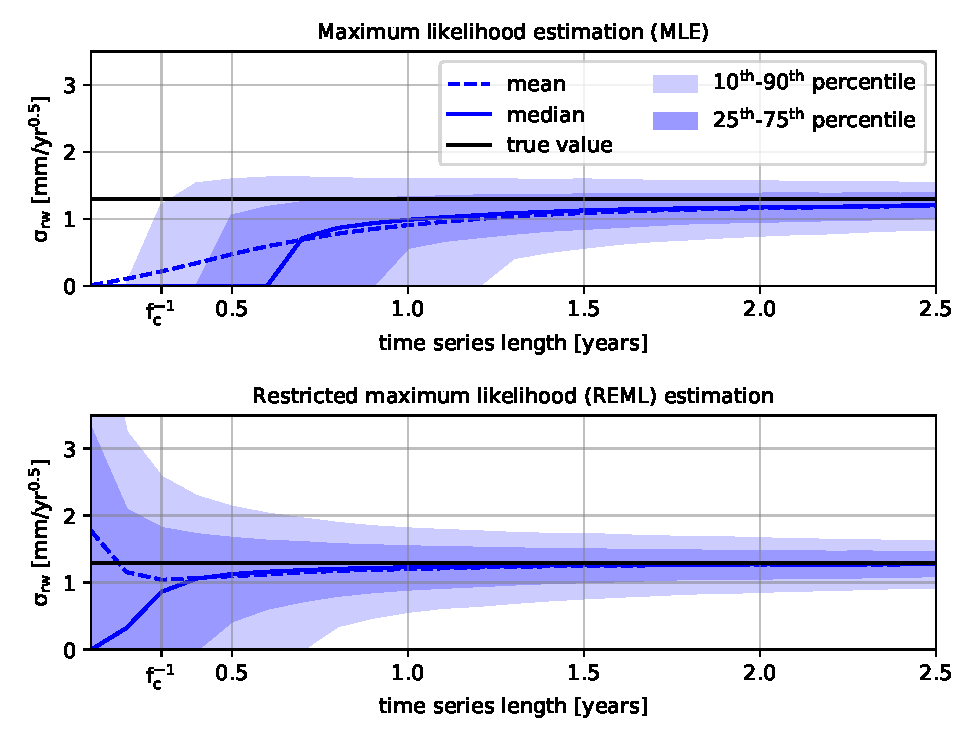
\includegraphics{ch4/figures/fig1.pdf}
\caption{Random walk amplitudes, $\sigma_{rw}$, estimated by the MLE and REML methods from synthetic data. The length of the synthetic time series used to estimate $\sigma_{rw}$ is varied from 0.1 yr to 2.5 yr. The black line indicates the true random walk amplitude ($\sigma_{rw}=1.3$), the light blue region shows the 10-90 percentile of estimates, the dark blue region shows the 25-75 percentile of estimates, the solid blue line indicates the median, and the dashed blue line indicates the mean.}   
\label{ch4:fig:1}
\end{figure}

The distribution of $\sigma_{rw}$ estimated by the MLE method indicates that there is a bias towards underestimating $\sigma_{rw}$ when the length of the time series is comparable to $f_c^{-1}$, which is 0.3 yr in this demonstration. The bias is appreciable when the time series is shorter than ${\sim}1$ yr, and estimates of $\sigma_{rw}$ cluster around 0.0 when the time series is shorter than $f_c^{-1}$. The distribution tightens up around the true value and remains relatively constant for time series with length greater than ${\sim}1$ yr. This is consistent with \citet{Langbein1997} who said that the time series should be at least 5 times greater than $f_c^{-1}$ to get a good estimate of the random walk component. Even when the full length of the time series is used, the mean and median of the distribution tend to be slightly less than the true value.

In contrast, the REML method does significantly better at estimating $\sigma_{rw}$. For every time series length considered, the true value for $\sigma_{rw}$ is within the 25-75 percentile of estimated $\sigma_{rw}$. For time series longer than $f_c^{-1}$, the mean and median of estimated $\sigma_{rw}$ closely resembles the true value, indicating that the REML method is indeed unbiased. When the length of the time series is less than $f_c^{-1}$, the mean and median deviate from the true value and the variance of estimated $\sigma_{rw}$ sharply increases. For such short time series, the random walk component cannot be resolved because it is being masked by the white noise.

\section{Discussion and conclusion}\label{ch4:sec:conclusion}
The MLE method is the most commonly used method for quantifying noise in geodetic time series, despite the fact that it is known to be biased. The bias in the MLE method can result in underestimated uncertainties in geophysical parameters derived from geodetic time series \citep{Langbein2012}. The intention of this paper is to bring the REML method to light in the geodetic community as an unbiased alternative. Since the MLE method is well established, it may not be reasonable to suggest that researchers abandon it in favor of the REML method.  However, the REML method is nearly identical to the MLE method in terms of its computational cost and in terms of its implementation. Indeed, the only difference between the log likelihood functions being maximized by the REML and MLE methods is that the REML method includes two additional, easily computed, terms (See Appendix 4A). We can therefore view the REML method as merely an unbiased correction to the MLE method.     

In this paper, we have used synthetic tests to demonstrate that the REML method does not suffer from the bias inherent in the MLE method from \citet{Langbein1997}. We show that the REML method is able to characterize random walk noise in geodetic time series that are as short at $f_c^{-1}$. In contrast, the MLE method can only accurately quantify random walk noise for time series that are several times longer than $f_c^{-1}$. We believe that the REML method should always be preferred over the MLE method for quantifying noise in geodetic time series. 

\section{Acknowledgements}
This material is based upon work supported by the National Science Foundation under grant EAR 1245263.

\bibliographystyle{agu04}  
\bibliography{refs}   % name your BibTeX data base

\newappendix{Appendix 4A: REML algorithm}
Algorithm 1 demonstrates how to efficiently compute the log of the REML likelihood function. For comparison, we include Algorithm 2, which evaluates the log of the MLE likelihood function. If we assume that $m \ll n$, then the main computational burden in both algorithms is computing the Cholesky decomposition of $\mathbf{\Sigma}$. Since we are just interested in finding the $\mathbf{\Sigma}$ that maximizes these functions, we can omit the terms in the log likelihood functions that are independent of $\mathbf{\Sigma}$. In that case, the only difference between the two algorithms is that Algorithm 1 includes a summation along the diagonals of $\mathbf{C}$ in the log likelihood function.    

\begin{algorithm}\label{ch4:alg:1}
\caption{Function that takes $\mathbf{d}$, $\mathbf{\Sigma}$, and $\mathbf{G}$ as input and returns the logarithm of eq. (\ref{ch4:eq:reml}). We use the notation $\mathbf{X} \backslash \mathbf{Z}$ to denote solving the system of equations $\mathbf{XY} = \mathbf{Z}$ for $\mathbf{Y}$.} 
\begin{algorithmic}
\Function{$reml\_log\_likelihood$}{$\mathbf{d}$,$\mathbf{\Sigma}$,$\mathbf{G}$}
\State $\mathbf{A} \gets cholesky(\mathbf{\Sigma})$ 
\State $\mathbf{B} \gets \mathbf{A} \backslash \mathbf{G}$
\State $\mathbf{C} \gets cholesky(\mathbf{B}^T\mathbf{B})$
\State $\mathbf{D} \gets cholesky(\mathbf{G}^T\mathbf{G})$
\State $\mathbf{a} \gets \mathbf{A} \backslash \mathbf{d}$
\State $\mathbf{b} \gets \mathbf{C} \backslash (\mathbf{B}^T\mathbf{a})$
\State \Return $\sum_i^m \log(D_{ii}) - 
                \sum_i^n \log(A_{ii}) - 
                \sum_i^m \log(C_{ii}) - 
                \frac{1}{2}\mathbf{a}^T\mathbf{a} + 
                \frac{1}{2}\mathbf{b}^T\mathbf{b} -
                \frac{n-m}{2}\log(2\pi)$
\EndFunction
\end{algorithmic}
\end{algorithm}

\begin{algorithm}\label{ch4:alg:2}
\caption{Function that takes $\mathbf{d}$, $\mathbf{\Sigma}$, and $\mathbf{G}$ as input and returns the logarithm of eq. (\ref{ch4:eq:mle}).} 
\begin{algorithmic}
\Function{$mle\_log\_likelihood$}{$\mathbf{d}$,$\mathbf{\Sigma}$,$\mathbf{G}$}
\State $\mathbf{A} \gets cholesky(\mathbf{\Sigma})$ 
\State $\mathbf{B} \gets \mathbf{A} \backslash \mathbf{G}$
\State $\mathbf{C} \gets cholesky(\mathbf{B}^T\mathbf{B})$
\State $\mathbf{a} \gets \mathbf{A} \backslash \mathbf{d}$
\State $\mathbf{b} \gets \mathbf{C} \backslash (\mathbf{B}^T\mathbf{a})$
\State \Return $-\sum_i^n \log(A_{ii}) - 
                \frac{1}{2}\mathbf{a}^T\mathbf{a} + 
                \frac{1}{2}\mathbf{b}^T\mathbf{b} -
                \frac{n}{2}\log(2\pi)$
\EndFunction
\end{algorithmic}
\end{algorithm}





\chapter{Revealing transient strain in geodetic data with Gaussian process regression}

\section{Summary}
Transient strain rates derived from GNSS data can be used to detect and understand geophysical phenomena such as slow slip events and postseismic deformation. Here we propose using Gaussian process regression (GPR) as a tool for estimating transient strain rates from GNSS data. GPR is a non-parametric, Bayesian method for interpolating scattered data. Transient strain rates estimated with GPR have meaningful uncertainties, allowing geophysical signal to be easily discerned from noise. In our approach, we assume a stochastic prior model for transient displacements. The prior describes how much one expects transient displacements to covary spatially and temporally. A posterior estimate of transient strain rates is obtained by differentiating the posterior displacements. One limitation with GPR is that it is not robust against outliers, so we introduce a pre-processing method for detecting and removing outliers in GNSS data. As a demonstration, we use GPR to detect transient strain resulting from slow slip events in Cascadia. Maximum likelihood methods are used to constrain a prior model for transient displacements in this region. The temporal covariance of our prior model is described by a compact Wendland covariance function, which significantly reduces the computational burden that can be associated with GPR. Our results reveal the spatial and temporal evolution of strain from slow slip events. We verify that the transient strain estimated with GPR is in fact geophysical signal by comparing it to the seismic tremor that is associated with Cascadia slow slip events.

\section{Introduction}\label{ch5:sec:Introduction}
Crustal strain rates are fundamentally important quantities for assessing seismic hazard. Knowing where and how quickly strain is accumulating gives insight into where we can expect stored elastic energy to be released seismically. Consequently, secular crustal strain rates estimated from GNSS data have been used to constrain seismic hazard models such as UCERF3 \citep{Field2014}. Transient crustal strain, which is caused by geophysical phenomena such as slow slip events (SSEs) or postseismic deformation, is also relevant for assessing seismic hazard. While transient strain itself is not damaging, there is a risk that it can trigger major earthquakes \citep{Roeloffs2006,Freed2001}. Dense networks of continuous GNSS stations, such as the Plate Boundary Observatory (PBO), make it possible to identify transient strain with high fidelity. Developing and improving upon methods for deriving secular and transient strain from GNSS data is an active area of research.

Most methods for estimating strain rates from GNSS data assume some parametric form of the deformation signal. The simplest method for estimating secular strain rates assumes that GNSS derived velocities can be described with a first-order polynomial (i.e., having constant deformation gradients) over some subnetwork of the GNSS stations \citep[e.g.,][]{Feigl1990,Murray2000}. The components of the strain rate tensor  for each subnetwork are then determined through a least squares fit to the observations. The assumption that deformation gradients are spatially uniform is not appropriate when subnetworks span too large of an area. To help overcome this deficiency, \citet{Shen1996,Shen2015} used an inverse distance weighting scheme, in which the estimated strain rate at some point is primarily controlled by observations at nearby stations. However, the methods described in \citet{Shen1996,Shen2015} are still formulated by assuming that the deformation gradients are uniform over the entire network. The errors in this assumption manifest as implausibly low formal uncertainties for the estimated strain rates. Other methods for estimating secular strain rates have parameterized GNSS derived velocities with bi-cubic splines \citep{Beavan2001}, spherical wavelets \citep{Tape2009}, and elastostatic Green's functions \citep{Sandwell2016}. The type of basis functions and the number of degrees of freedom for a parameterization can be subjective. If there are too few degrees of freedom in the parameterization, then estimated strain rates will be biased and the uncertainties will be underestimated. On the other hand, if there are too many degrees of freedom, then there will not be any coherent features in the estimated strain rates. The methods described by \citet{Beavan2001} and \citet{Tape2009} also require the user to specify penalty parameters that control a similar trade-off between bias and variance in the solution. One could parameterize deformation with a physically motivated model of interseismic deformation \citep[e.g.,][]{Meade2005,McCaffrey2007}. In such models the lithospheric rheology and fault geometries are assumed to be known. Any errors in the assumed physical model could result in biased strain estimates and underestimated formal uncertainties. 

The aforementioned studies are concerned with estimating secular strain rates. In recent years the Southern California Earthquake Center (SCEC) community has shown interest in developing methods for detecting transient strain. SCEC supported a transient detection exercise \citep{Lohman2013}, where several research groups tested their methods for detecting transient geophysical signal with a synthetic GNSS dataset. Among the methods tested were the Network Strain Filter (NSF) \citep{Ohtani2010} and the Network Inversion Filter (NIF) \citep{Segall1997}. The NSF uses a wavelet parameterization to  describe the spatial component of geophysical signal. The NIF, which is intended for imaging slow fault slip from geodetic data, uses the elastic dislocation Green's functions from \citet{Okada1992}. For the NSF and NIF, the time dependence of the geophysical signal is modeled as integrated Brownian motion. The method described in \citet{Holt2013} was also tested in the SCEC transient detection exercise, which calculates strain rates using a bi-cubic spatial parameterization of displacements between time epochs. \citet{Holt2013} defined a detection threshold based on the strain rate magnitude, and below we demonstrate that this is indeed an effective criterion for identifying geophysical signal. For the same reasons descibed above, the transient deformation and corresponding uncertainties estimated by these methods can be biased by the chosen spatial parameterization. It is then difficult to distinguish signal from noise with these methods, which limits their utility for transient detection.   

Here we propose using Gaussian process regression (GPR) \citep{Rasmussen2006} to estimate transient strain from GNSS data. GPR is a Bayesian, non-parametric method for inferring a continuous signal from scattered data. Since GNSS stations are irregularly spaced and observation times may differ between stations, GPR is an ideal tool for synthesizing GNSS data into a spatially and temporally continuous representation of surface deformation. GPR is closely related to kriging \citep{Cressie1992} and least squares collocation \citep{Moritz1978}. The latter has been used by \citet{Kato1998} and \citet{El-Fiky1999} to estimate secular strain rates from GNSS data. GPR is Bayesian in that we describe our prior understanding of the geophysical signal with a Gaussian process. A Gaussian process is a normally distributed stochastic process that is fully defined in terms of a mean function and a positive definite covariance function. For example, Brownian motion, $B(t)$, is a well known Gaussian process in $\mathbb{R}^1$ which has zero mean and covariance function $\mathrm{cov}(B(t),B(t')) = \min(t,t')$, where $t,t' \ge 0$. If no prior information is available for the geophysical signal, then maximum likelihood methods can be used to objectively choose a prior Gaussian process that is most consistent with the observations.  We incorporate GNSS observations with the prior to form a posterior estimate of transient strain.  The posterior transient strain is also a Gaussian process, and we can use its distribution to confidently discern geophysical signal from noise. We use GPR to infer strain resulting from SSEs in Cascadia, demonstrating that GPR is an effective tool for detecting transient geophysical processes. 

\section{Estimating transient strain rates}\label{ch5:sec:Method}
We seek a spatially and temporally dependent estimate of transient crustal strain rates. We consider transient strain rates to be any deviation from secular strain rates, and our attention is limited to horizontal strain rates in this study. We denote transient crustal strain rates as $\dot\varepsilon(p)$, where $p$ represents the ordered pair $(\vec{x},t)$, $\vec{x}$ are spatial coordinates in $\mathbb{R}^2$, and $t$ is time. We determine $\dot\varepsilon(p)$ by spatially and temporally differentiating estimates of transient displacements, $\vec{u}(p)$. We make a prior assumption that each component of $\vec{u}$ is a Gaussian process,
\begin{equation}\label{ch5:eq:TransientDeformation}
u_i(p) \sim \mathcal{N}\left(0,C_{u_i}\right),
\end{equation}
where $C_{u_i}(p,p')$ is a covariance function indicating how we expect $u_i(p)$ to covary with $u_i(p')$. For simplicity, we treat each component of displacements independently and ignore any potential covariance between them. Hence, we drop the component subscripts with the understanding that the same analysis is being repeated to estimate the easting and northing components of $\vec{u}$. We assume that $C_u$ can be separated into spatial and temporal functions as 
\begin{equation}\label{ch5:eq:TransientCovariance}
C_{u}\left((\vec{x},t),(\vec{x}',t')\right) = X(\vec{x},\vec{x}')T(t,t').
\end{equation}  
As long as the functions $X$ and $T$ are positive definite, $C_u$ is guaranteed to also be positive definite and thus a valid covariance function \citep[sec. 4.2.4]{Rasmussen2006}. The appropriate choice for $X$ and $T$ may vary depending on the geophysical signal we are trying to describe, and we discuss this matter in Section \ref{ch5:sec:SignalModel}.  

We constrain $u$ with GNSS data, which records $u$ as well as other physical and non-physical processes that we are not interested in. We describe GNSS observations at position $\vec{x}_i$ and time $t_j$ as a realization of the random variable 
\begin{align}\label{ch5:eq:Data}
\begin{split}
d_{ij} = &u(\vec{x}_i,t_j) + \eta(\vec{x}_i,t_j) + w_{ij} + a^{(1)}_i + a^{(2)}_it_j + \\
         &a^{(3)}_i\sin(2 \pi t_j) + a^{(4)}_i\cos(2 \pi t_j) + a^{(5)}_i\sin(4 \pi t_j) + a^{(6)}_i\cos(4 \pi t_j), 
\end{split}
\end{align}
where $a^{(1)}_{i}$ is an offset that is unique for each GNSS monument, $a^{(2)}_{i}$ is the secular velocity at $\vec{x}_i$, and the sinusoids describe seasonal deformation (using units of years for $t_j$). We use $w_{ij}$ to denote normally distributed, uncorrelated noise. Correlated noise which does not have a parametric representation is denoted by $\eta$.  For example, $\eta$ can consist of temporally correlated noise describing benchmark wobble \citep[e.g.,][]{Wyatt1982,Wyatt1989}, and/or spatially correlated noise describing common mode error \citep[e.g.,][]{Wdowinski1997}. For now, we will only assume that $\eta \sim \mathcal{N}(0,C_\eta)$. We consider the six coefficients in eq. (\ref{ch5:eq:Data}) to be uncorrelated random variables distributed as $\mathcal{N}(0,\kappa^2)$ in the limit as $\kappa \to \infty$ (i.e., the coefficients have diffuse priors). Of course, the secular velocities, $a^{(2)}_{i}$, are spatially correlated and we could invoke a tectonic model to form a prior on $a^{(2)}_{i}$. However, in our application to Cascadia, we will be using displacement time series which are long enough to sufficiently constrain $a^{(2)}_{i}$ for each station, avoiding the need to incorporate a prior. Likewise, seasonal deformation is spatially correlated \citep{Dong2002,Langbein2008}, and it may be worth exploring and exploiting such a correlation in a future study. 

We now consider the column vector of $n$ GNSS observations made at $m$ stations, $\mathbf{d}_*$. Let $\mathbf{P}$ be the set of $(\vec{x}_i, t_j)$ pairs describing where and when each of the GNSS observations have been made. Let $\mathbf{a}$ be the vector of coefficients from eq. (\ref{ch5:eq:Data}) for each of the $m$ GNSS stations. We use $\mathbf{G}$ to represent the $n \times 6m$ matrix of corresponding basis functions evaluated at each point in $\mathbf{P}$. We  also denote the vector of uncorrelated noise for each observation as $\mathbf{w}$, whose standard deviations are given by the formal data uncertainty, $\mathbf{\sigma}$. The observations can then be viewed as a realization of the random vector
\begin{equation}
\mathbf{d} = u(\mathbf{P}) + \eta(\mathbf{P}) + \mathbf{w} + \mathbf{G}\mathbf{a},
\end{equation}
which is distributed as $\mathcal{N}(\mathbf{0},\mathbf{\Sigma} + \kappa^2\mathbf{G}\mathbf{G}^T)$, where
\begin{equation}\label{ch5:eq:Cd}
\mathbf{\Sigma} = C_u(\mathbf{P},\mathbf{P}) + C_\eta(\mathbf{P},\mathbf{P}) + 
              \mathrm{diag}\left(\mathbf{\sigma}^2\right).  
\end{equation}
It should be understood that notation such as $u(\mathbf{P})$ and $C_u(\mathbf{P},\mathbf{P})$ represents the column vector $[u(P_i)]_{P_i \in \mathbf{P}}$ and the matrix $[C_u(P_i,P_j)]_{(P_i,P_j) \in \mathbf{P} \times \mathbf{P}}$, respectively. 

The prior for transient displacements is then conditioned with $\mathbf{d}_*$ to form a posterior estimate of transient displacements, $\hat{u} = u | \mathbf{d}_*$. For now, we will assume that appropriate covariance functions and corresponding hyperparameters for $C_u$ and $C_\eta$ have already been chosen. In Section \ref{ch5:sec:NoiseModel} and \ref{ch5:sec:SignalModel}, we discuss how the covariance functions are chosen for our application to GNSS data from Cascadia. If $\kappa$ is kept finite then, from \citet[sec. 2.2]{Rasmussen2006}, we find that $\hat{u}$ is distributed as $\mathcal{N}(\mu_{\hat{u}},C_{\hat{u}})$, where
\begin{equation}\label{ch5:eq:PosteriorMean}
\mu_{\hat{u}}(p) = C_u(p,\mathbf{P})\left(\mathbf{\Sigma} + \kappa^2\mathbf{G}\mathbf{G}^T\right)^{-1}\mathbf{d}_*
\end{equation}    
and
\begin{equation}\label{ch5:eq:PosteriorCov}
C_{\hat{u}}(p,p') = C_u(p,p') - C_u(p,\mathbf{P})\left(\mathbf{\Sigma} + \kappa^2\mathbf{G}\mathbf{G}^T\right)^{-1}C_u(\mathbf{P},p').
\end{equation}
However, we are interested in the limit as $\kappa \to \infty$, and the form for eq. (\ref{ch5:eq:PosteriorMean}) and eq. (\ref{ch5:eq:PosteriorCov}) is not suitable for evaluating this limit. We use a partitioned matrix inversion identity \citep[sec. 2.7.4]{Press2007} to rewrite eq. (\ref{ch5:eq:PosteriorMean}) and eq. (\ref{ch5:eq:PosteriorCov}) as
 \begin{equation}\label{ch5:eq:PosteriorMean2}
\mu_{\hat{u}}(p) = \left[\begin{array}{cc}
                         C_u(p,\mathbf{P}) & \mathbf{0} \\
                         \end{array}\right]
                   \left[\begin{array}{cc}
                         \mathbf{\Sigma} & \mathbf{G} \\
                         \mathbf{G}^T  & -\kappa^{-2} \mathbf{I} \\
                         \end{array}\right]^{-1}
                   \left[\begin{array}{c}
                         \mathbf{d}_* \\
                         \mathbf{0} \\
                         \end{array}\right]
\end{equation}    
and
\begin{equation}\label{ch5:eq:PosteriorCov2}
C_{\hat{u}}(p,p') = C_u(p,p') - 
                    \left[\begin{array}{cc}
                          C_u(p,\mathbf{P}) & \mathbf{0} \\
                          \end{array}\right]
                    \left[\begin{array}{cc}
                          \mathbf{\Sigma} & \mathbf{G} \\
                          \mathbf{G}^T  & -\kappa^{-2} \mathbf{I} \\
                          \end{array}\right]^{-1}
                    \left[\begin{array}{c}
                          C_u(\mathbf{P},p') \\
                          \mathbf{0} \\
                          \end{array}\right].
\end{equation}
Taking the limit as $\kappa \to \infty$, we get the solution for the mean and covariance of $\hat{u}$,
 \begin{equation}\label{ch5:eq:PosteriorMean3}
\mu_{\hat{u}}(p) = \left[\begin{array}{cc}
                         C_u(p,\mathbf{P}) & \mathbf{0} \\
                         \end{array}\right]
                   \left[\begin{array}{cc}
                         \mathbf{\Sigma} & \mathbf{G} \\
                         \mathbf{G}^T  & \mathbf{0} \\
                         \end{array}\right]^{-1}
                   \left[\begin{array}{c}
                         \mathbf{d}_* \\
                         \mathbf{0} \\
                         \end{array}\right]
\end{equation}    
and
\begin{equation}\label{ch5:eq:PosteriorCov3}
C_{\hat{u}}(p,p') = C_u(p,p') - 
                    \left[\begin{array}{cc}
                          C_u(p,\mathbf{P}) & \mathbf{0} \\
                          \end{array}\right]
                    \left[\begin{array}{cc}
                          \mathbf{\Sigma} & \mathbf{G} \\
                          \mathbf{G}^T  & \mathbf{0} \\
                          \end{array}\right]^{-1}
                    \left[\begin{array}{c}
                          C_u(\mathbf{P},p') \\
                          \mathbf{0} \\
                          \end{array}\right].
\end{equation}

We use eq. (\ref{ch5:eq:PosteriorMean3}) and (\ref{ch5:eq:PosteriorCov3}) to find the posterior easting and northing components of transient displacements. Using $\hat{u}_i$ to denote the posterior transient displacements along direction $i$ and $x_i$ to represent the components of $\vec{x}$, we can write the components of $\dot\varepsilon$ as 
\begin{equation}\label{ch5:eq:StrainRate}
\dot\varepsilon_{ij}(p) = \frac{1}{2} \frac{\partial}{\partial t} \left(
                                        \frac{\partial \hat{u}_i(p)}{\partial x_j} +  
                                        \frac{\partial \hat{u}_j(p)}{\partial x_i}\right).
\end{equation}
The transient strain rate components are stochastic processes whose distributions can be interpreted as the distributions of samples of $\hat{u}$ that have been differentiated by the operator from eq. (\ref{ch5:eq:StrainRate}). Since differentiation is a linear operation, the transient strain rate components are Gaussian processes. From \citet[sec. 10.2]{Papoulis1991}, we find that the components of $\dot{\varepsilon}$ have mean functions
\begin{equation}\label{ch5:eq:StrainMean}
\mu_{\dot\varepsilon_{ij}}(p) = \frac{1}{2}\frac{\partial}{\partial t}\left(
                                  \frac{\partial \mu_{\hat{u}_i}(p)}{\partial x_j} + 
                                  \frac{\partial \mu_{\hat{u}_j}(p)}{\partial x_i} \right)
\end{equation} 
and covariance functions
\begin{equation}\label{ch5:eq:StrainCov}
C_{\dot\varepsilon_{ij}}(p,p') = \frac{1}{4} \frac{\partial^2}{\partial t \, \partial t'}\left(
                                   \frac{\partial^2 C_{\hat{u}_i}(p,p')}{\partial x_j \, \partial x'_j} + 
                                   \frac{\partial^2 C_{\hat{u}_j}(p,p')}{\partial x_i \, \partial x'_i} \right).
\end{equation} 

Our motivation for estimating transient strain rates is, in part, to detect geophysical phenomena. As we will see, geophysical signal can be easily identified by visually inspecting the solution for transient strain rates. However, if we want to detect geophysical phenomena automatically, then we need to define a detection criterion. We propose using a signal-to-noise ratio, SNR, based on $\dot\varepsilon$ for our detection criterion. The Frobenius norm of $\dot\varepsilon$, $||\dot\varepsilon||_\mathrm{F}$, which is sometimes referred to as the second invariant of strain rate in the geodetic literature, is often used as a metric for the strain rate ``magnitude''. Noting that $||\dot\varepsilon||_\mathrm{F}$ is a random variable, SNR can be taken as the ratio of the estimated mean and standard deviation of $||\dot\varepsilon||_\mathrm{F}$. Using nonlinear uncertainty propagation, we find SNR to be  
\begin{equation}\label{ch5:eq:SNR}
\mathrm{SNR}(p) = \frac{\mu_{\dot\varepsilon_\mathrm{nn}}(p)^2 +
                        \mu_{\dot\varepsilon_\mathrm{ee}}(p)^2 +
                        2\mu_{\dot\varepsilon_\mathrm{en}}(p)^2}
                       {\big(C_{\dot\varepsilon_\mathrm{nn}}(p,p)\mu_{\dot\varepsilon_\mathrm{nn}}(p)^2 + 
                              C_{\dot\varepsilon_\mathrm{ee}}(p,p)\mu_{\dot\varepsilon_\mathrm{ee}}(p)^2 + 
                              4C_{\dot\varepsilon_\mathrm{en}}(p,p)\mu_{\dot\varepsilon_\mathrm{en}}(p)^2
                        \big)^{\frac{1}{2}}}
,
\end{equation}
where the subscripts ``n'' and ``e'' denote north and east, respectively. For simplicity, we have ignored covariances between the transient strain rate components in eq. (\ref{ch5:eq:SNR}), even though they are non-zero.  

\section{Outlier detection}\label{ch5:sec:Outlier}
In our formulation for estimating transient strain rates, we have assumed that noise in the data vector is normally distributed. This is not an appropriate assumption for GNSS data, which often have more outliers than would be predicted for normally distributed noise. It follows that proposed methods for analyzing GNSS data should be robust against outliers \citep[e.g.,][]{Blewitt2016}. In order to make our estimates of transient strain more robust, we automatically identify and remove outliers in the GNSS data as a pre-processing step.

Our method for detecting outliers is based on the data editing algorithm described in \citet{Gibbs2011}. We calculate the residuals between the observations and a best fitting model. Data with residuals that are anomalously large are then identified as outliers. We treat $\mathbf{d}_*$ as a sample of $\mathbf{d}$ and assume that there is no correlated noise (i.e., $\eta(p) = 0$).  The best fitting model for $\mathbf{d}_*$ is considered to be the expected value of the random vector $u(\mathbf{P}) + \mathbf{G}\mathbf{a}$ after conditioning it with non-outlier observations.  We still consider $u$ to have a separable covariance function as in eq. (\ref{ch5:eq:TransientCovariance}), and the choice for $X$ and $T$ does not need to be the same as that used in Section \ref{ch5:sec:Method}. Since outliers are determined based on how well a spatially and temporally dependent model fits the data, we are able to identify anomalous observations which may not be immediately apparent from inspecting individual time series. 

To begin the algorithm, we let $\mathbf{\Omega}$ be the index set of non-outliers in $\mathbf{d}_*$ and initiate it with all $n$ indices. This algorithm is iterative, and for each iteration we calculate the residual vector
\begin{align}\label{ch5:eq:Residual}
\mathbf{r} &= \frac{\mathbf{d}_* - \mathrm{E}\left[(u(\mathbf{P}) + \mathbf{G}\mathbf{a})|\tilde{\mathbf{d}}_* \right]}{\mathbf{\sigma}} \\
       &= \frac{1}{\mathbf{\sigma}}\left(\mathbf{d}_*  - 
          \left[\begin{array}{cc}
                C_u(\mathbf{P},\tilde{\mathbf{P}}) & \mathbf{G} \\
                \end{array}\right]
          \left[\begin{array}{cc}
                C_u(\tilde{\mathbf{P}},\tilde{\mathbf{P}}) + \mathrm{diag}(\tilde{\mathbf{\sigma}}^2) & \tilde{\mathbf{G}} \\
                \tilde{\mathbf{G}}^T  & \mathbf{0} \\
                \end{array}\right]^{-1}
          \left[\begin{array}{c}
                \tilde{\mathbf{d}}_* \\
                \mathbf{0} \\
                \end{array}\right]\right),
\end{align}
where the tilde indicates that only elements corresponding to indices in $\mathbf{\Omega}$ are retained (e.g., $\tilde{\mathbf{P}} = \{P_i\}_{i\in\mathbf{\Omega}}$). We then update $\mathbf{\Omega}$ to be
\begin{equation}\label{ch5:eq:Update}
\mathbf{\Omega} = \{i : |r_i| < \lambda \cdot \mathrm{RMS}\}, \ \ \ r_i \in \mathbf{r},
\end{equation} 
where RMS is the root-mean-square of $\tilde{\mathbf{r}}$ and $\lambda$ is an outlier tolerance. We use $\lambda=4$ in this study, which in our experience accurately identifies outliers without unnecessarily decimating the data. Iterations continue until the new $\mathbf{\Omega}$ is equal to the previous $\mathbf{\Omega}$. 

It should be noted that this algorithm does not identify jumps in GNSS time series, which are another common issue. Some, but not all, jumps can be automatically removed by looking up the dates of equipment changes and earthquakes. However, it is still necessary to manually find and remove jumps of unknown origin. That being said, this outlier detection algorithm significantly reduces the effort needed to manually clean GNSS data.       

\section{Application to Cascadia slow slip events}\label{ch5:sec:Cascadia}
We use our method to estimate transient strain rates in Cascadia, and we are specifically interested in identifying strain resulting from SSEs \citep[e.g.,][]{Dragert2001}. In Cascadia, SSEs can be detected by monitoring for associated seismic tremor \citep{Rogers2003}, which is actively being done by the Pacific Northwest Seismic Network \citep{Wech2010}. We can thus compare the tremor records to the transient strain rates estimated with GPR to verify that we are indeed identifying strain from SSEs.  

We use the daily displacement solutions generated by the Geodesy Advancing Geosciences and EarthScope (GAGE) facility for continuous GNSS stations \citep{Herring2016}. This data is publicly available and can be found at www.unavco.org. We limit the dataset to the stations and time ranges which are pertinent to the seven most recent SSEs in the Puget Sound region. The earliest SSE considered in this study began in August 2010, and the most recent SSE began in February 2017. We use these most recent SSEs because the station coverage is sufficiently dense for us to use maximum likelihood methods to constrain prior models.  The positions of GNSS stations used to estimate transient strain rates are shown in Figure \ref{ch5:fig:Context}.  

\begin{figure*}
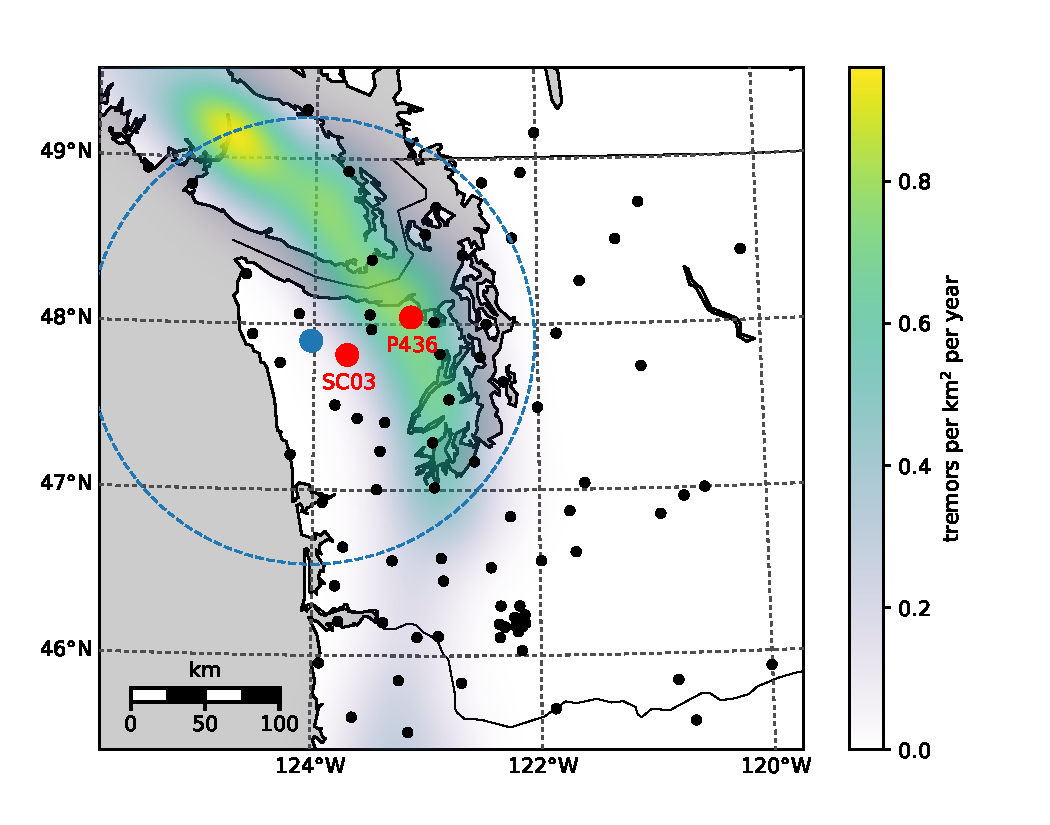
\includegraphics{ch5/figures/context_map/context-map.pdf}
\caption{Positions of continuous GNSS stations used to estimate transient strain rates. The colored regions indicate the distribution of seismic tremor as determined by \citet{Wech2010}. The red dots show the positions of GNSS stations mentioned in this paper. The blue dot indicates the location of the transient strain rates shown in Figure \ref{ch5:fig:StrainTs} and the signal-to-noise ratio shown in Figure \ref{ch5:fig:StrainMag}. The blue dashed circle demarcates the spatial extent of the tremors shown in Figure \ref{ch5:fig:StrainMag}.}    
\label{ch5:fig:Context}
\end{figure*}

\subsection{Noise model}\label{ch5:sec:NoiseModel}
Before we determine the transient strain rates, we must establish a prior for the transient displacements, $u$, and the noise, $\eta$. In this section we discuss our choice for the noise covariance function $C_\eta$. There have been numerous studies on temporally correlated noise in GNSS data \citep[e.g.,][]{Zhang1997,Mao1999,Williams2004,Langbein2008}. In these studies, temporally correlated noise was described with some combination of Brownian motion, a first-order Gauss-Markov (FOGM) process, and/or flicker noise. There is some physical justification for using Brownian motion as a noise model because it accurately describes the power spectrum of motion resulting from instability in geodetic monuments \citep[e.g.,][]{Wyatt1982,Wyatt1989}. Here we describe the time dependence of $\eta$ as a FOGM process and consider $\eta$ to be spatially uncorrelated. A FOGM process is a solution to the stochastic differential equation
\begin{equation}\label{ch5:eq:FOGMdef}
\dot{\eta}(t) + \alpha \eta(t) = \beta w(t),
\end{equation}
where $w(t)$ is white noise with unit variance. The FOGM process degenerates to the commonly used Brownian motion noise model under the condition that $\alpha=0$ and $\eta(0) = 0$. Our noise model that satisfies eq. (\ref{ch5:eq:FOGMdef}) is a Gaussian process with zero mean and the covariance function
\begin{equation}\label{ch5:eq:FOGM}
C_\eta\left((\vec{x},t),(\vec{x}',t')\right) = \frac{\beta^2}{2\alpha}\exp\left(-\alpha|t - t'|\right) \delta(||\vec{x} - \vec{x}'||_2). 
\end{equation}

We constrain the hyperparameters for $\eta$, $\alpha$ and $\beta$, with a set of 38 continuous GNSS stations in Cascadia that are east of 121$^\circ$W.  These stations are sufficiently far from the subduction zone that they are unlikely to contain transient signal associated with SSEs.  We clean the data for these stations by removing jumps at times of equipment changes, and we remove outliers that have been detected with the algorithm described in Section \ref{ch5:sec:Outlier}. We then find $\alpha$ and $\beta$ for each station time series with the Restricted Maximum Likelihood (REML) method \cite[e.g.,][]{Harville1974,Cressie1992,Hines2017}. The REML method finds the hyperparameters, which we collectively refer to as $\mathbf{\theta}$, that maximize the likelihood function
\begin{equation}\label{ch5:eq:REML}
\mathcal{L}(\mathbf{\theta}) = \left(\frac{\left|\mathbf{G}^T\mathbf{G}\right|}
                           {(2\pi)^{n-6m} 
                           \left| \mathbf{\Sigma}(\mathbf{\theta}) \right| 
                           \left| \mathbf{G}^T\mathbf{\Sigma}(\mathbf{\theta})^{-1}\mathbf{G} \right|}\right)^{\frac{1}{2}} 
                           e^{-\tfrac{1}{2}\mathbf{d}_*^T\mathbf{K}(\mathbf{\theta})\mathbf{d}_*},
\end{equation}
where
\begin{equation}
\mathbf{K}(\mathbf{\theta}) = \mathbf{\Sigma}(\mathbf{\theta})^{-1} - 
                      \mathbf{\Sigma}(\mathbf{\theta})^{-1}\mathbf{G}
         \left(\mathbf{G}^T\mathbf{\Sigma}(\mathbf{\theta})^{-1}\mathbf{G}\right)^{-1}
         \mathbf{G}^T\mathbf{\Sigma}(\mathbf{\theta})^{-1}.
\end{equation}
\citet{Harville1974} showed that choosing the hyperparameters which maximize eq. (\ref{ch5:eq:REML}) is equivalent to choosing the hyperparameters which maximize the probability of drawing $\mathbf{d}_*$ from $\mathbf{d}$. We use the REML method over the maximum likelihood method \citep[e.g.,][]{Langbein1997} because the REML method accounts for the improper prior that we assigned to $\mathbf{a}$ \citep{Hines2017}. We independently estimate $\mathbf{\theta}$ for each station, and so $\mathbf{d}_*$ consists of displacements for an individual station. We are assuming $u(p)=0$ when estimating the noise hyperparameters for this section. The distribution of inferred $\alpha$ and $\beta$ are shown in Figure \ref{ch5:fig:NoiseParams}. The amplitude of FOGM noise, $\beta$, for the easting and northing components is notable low and are clustered around 0.5 mm/yr$^{0.5}$. The corresponding estimates of $\alpha$ tend to cluster around 0 yr$^{-1}$, suggesting that noise can be described with Brownian motion. We also estimate hyperparameters for the vertical component of displacements, under the hope that vertical deformation gradients could reveal some geophysical signal. The amplitude of FOGM noise for the vertical component is relatively large with a median value of 13.5 mm/yr$^{0.5}$.  The inferred values for $\alpha$ are also higher for the vertical component with a median value of 8.21 yr$^{-1}$. In Figure \ref{ch5:fig:NoiseSamples}, we use the median values of $\alpha$ and $\beta$ to generate two random samples of FOGM noise for each component. The samples span five years and over these five years the easting and northing samples drift by about 1 mm. In the context of detecting SSEs, which produce several mm's of surface displacement on the time-scale of weeks, the estimated FOGM noise for the easting and northing component is negligible. In contrast, the estimated FOGM noise for the vertical component is larger than the signal we would expect from SSEs. We suspect that the higher amplitude for the FOGM noise in the vertical component is accommodating for deficiencies in our rather simple seasonal model. Based on this analysis, we henceforth ignore temporally correlated noise in the easting and northing component because of its low amplitude. We also do not use vertical displacements because of the presumably low signal-to-noise ratio.

\begin{figure*}
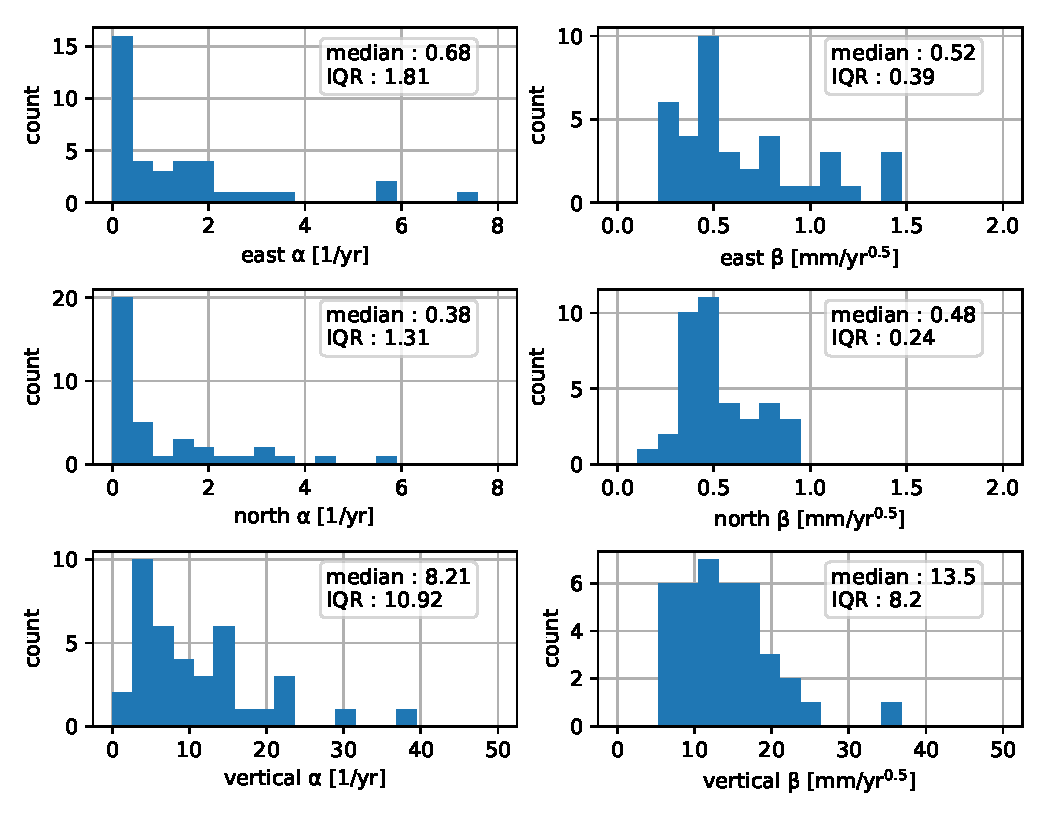
\includegraphics{ch5/figures/noise/noise-params.pdf}
\caption{Distribution of estimated FOGM hyperparameters (eq. \ref{ch5:eq:FOGM}). Hyperparameters are estimated with the REML method for 38 stations in Cascadia that are east of $121^\circ$W. ``IQR'' is the interquartile range.}   
\label{ch5:fig:NoiseParams}
\end{figure*}

\begin{figure*}
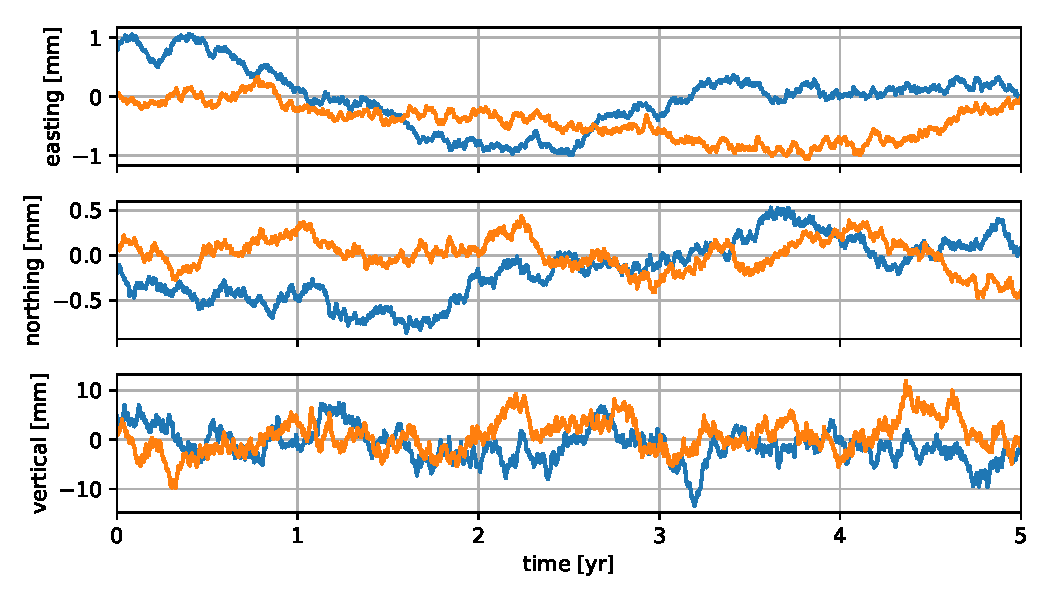
\includegraphics{ch5/figures/noise/noise-samples.pdf}
\caption{Two FOGM noise samples for each component. The FOGM hyperparameters have been set to the median values from Figure \ref{ch5:fig:NoiseParams}.}   
\label{ch5:fig:NoiseSamples}
\end{figure*}

Another significant source of noise in GNSS data is common mode error \citep[e.g.,][]{Wdowinski1997,Dong2006}, which is noise that is highly spatially correlated. When not accounted for, common mode error manifests as spatially uniform undulations in estimated transient displacements. However, estimated transient strain rates are insensitive to common mode error. We therefore do not include common mode error in our noise model. We then make the simplifying assumption that $\eta(p) = 0$ for the easting and northing component of GNSS data.  

\subsection{Prior model}\label{ch5:sec:SignalModel}
We next establish our prior model for transient displacements. Specifically, we discuss our choice for the covariance functions $X(\vec{x},\vec{x}')$ and $T(t,t')$. For $X$, we use the squared exponential (SE) covariance function,
\begin{equation}\label{ch5:eq:SE}
X(\vec{x},\vec{x}') = \exp\left(\frac{-||\vec{x} - \vec{x}'||_2^2}{2 \ell^2}\right).
\end{equation}
The SE covariance function is commonly used in kriging \citep[e.g,][]{Cressie1992} and Gaussian process regression \citep[e.g.,][]{Rasmussen2006}. The SE is a positive definite covariance function for any number of spatial dimensions. A Gaussian process with an SE covariance function is isotropic and has realizations that are infinitely differentiable. In terms of geodetic applications, \citet{Kato1998} and \cite{El-Fiky1999} demonstrated that the SE accurately describes the covariance of secular GNSS derived velocities in Japan.     

We consider three potential models for the temporal covariance of $u$. First, we consider the one-dimensional SE covariance function, 
\begin{equation}\label{ch5:eq:TimeSE}
T(t,t') = \phi^2\exp\left(\frac{-|t - t'|^2}{2\tau^2}\right).
\end{equation}
Note that $T$ includes the hyperparameter $\phi$, which serves to scale the covariance function $C_u$. Second, we consider integrated Brownian motion (IBM). IBM has zero mean and its covariance function can be found by integrating the covariance function for Brownian motion as
\begin{align}\label{ch5:eq:IBM}
T(t,t') &= \int_0^t \int_0^{t'} \phi^2 \min(s,s') \,ds'\,ds \\
        &= \frac{\phi^2}{2}\min(t,t')^2 \left(\max(t,t') - \frac{1}{3}\min(t,t')\right), \ \ \ t,t' \geq 0.
\end{align}
IBM has been used in the context of Kalman filtering as a non-parametric model for the time dependence of geophysical signals \citep[e.g.,][]{Segall1997,McGuire2003,Ohtani2010,Hines2016a}. It should be emphasized $t=0$ is a reference time at which the Gaussian process is exactly zero. For some geophysical signals, it is appropriate to have this reference time. For example, if we are trying to identify postseismic deformation then $t$ should be zero at the time of the earthquake.  However, if we are interesting in detecting transient events, where there is no known start time, then IBM may not be an appropriate prior, and an isotropic Gaussian process should be preferred. In the following analysis, we make the quite arbitrary choice that $t$ is zero on the first epoch of $\mathbf{d}_*$. Using an earlier reference time does not change the results discussed in this section. Our third option for $T$ is the Wendland class of covariance functions \citep{Wendland2005}. Wendland covariance functions have compact support and hence their corresponding covariance matrices are sparse. In our analysis, we exploit this sparsity with the CHOLMOD software package \citep{Chen2008}. Wendland functions are positive definite in $\mathbb{R}^d$, and they describes an isotropic Gaussian process with realizations that can be differentiated $k$ times. The form of the covariance function depends on the choice of $d$ and $k$. We use $d=1$ since we are describing the temporal covariance of $u$. We use $k=2$, giving samples of $u$ continuous velocities and accelerations. The corresponding Wendland covariance function is 
\begin{equation}\label{ch5:eq:Wendland}
T(t,t') = \phi^2\left(1 - \frac{|t - t'|}{\tau}\right)^5_+ \left(\frac{8|t - t'|^2}{\tau^2} + \frac{5|t - t'|}{\tau} + 1\right), 
\end{equation}
where
\begin{equation}
(t)_+ = 
\begin{cases}
t, \ \ \ t > 0 \\
0, \ \ \ \mathrm{otherwise}.
\end{cases}
\end{equation}

We next determine appropriate hyperparameters for $X$ and each of the three candidate covariance functions for $T$. First, we clean the GNSS datasets by removing offsets at times of equipment changes and removing outliers with the method describe in Section \ref{ch5:sec:Outlier}. For the outlier detection algorithm, our prior model, $u$, is chosen to have a length-scale and time-scale which is able to approximately describe SSE displacements. We use the SE covariance function for $X$ with length-scale $\ell = 100$ km, and we use the Wendland covariance function for $T$, due to its computational efficiency, with time-scale $\tau = 0.1$ yr and $\phi = 1$ mm.  The outlier detection algorithm is particularly effective at removing outliers for stations at high elevation (Figure \ref{ch5:fig:Outliers}), which can be adversely affected by ice or snow during the winter \citep{Lisowski2008}. After cleaning the dataset, we divide it into seven subsets which are four months long and each centered on the time of a SSE. The times of the seven SSEs are determined with tremor records from \cite{Wech2010}. We use the REML method to find the optimal hyperparameters for $T$ and $X$ for each subset of data. We choose to make each data subsets four months long because it is long enough to encompass a SSE in Cascadia, while it is short enough to still be computationally tractable. However, four months is too short to resolve the sinusoids in $\mathbf{d}$, and they are omitted from $\mathbf{d}$ in this REML analysis for Cascadia SSEs. The estimated hyperparameters for $u$ are summarized in Table 1. Based on the interquartile ranges, the estimated hyperparameters for the SE and Wendland covariance functions do not vary significantly between SSEs. This suggests that the median of estimated hyperparameters should be an appropriate prior model for all Cascadia SSEs. For the IBM model, there are several anomalously large values for $\ell$ and $\phi$, which results in large interquartile ranges.   

\begin{figure*}
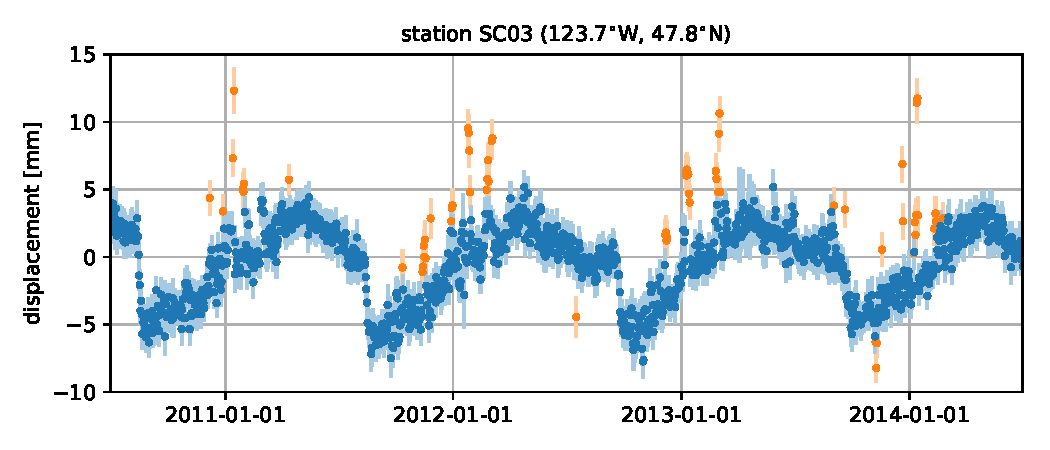
\includegraphics{ch5/figures/outliers/outliers.pdf}
\caption{Detrended easting component of displacements at station SC03, which is located on Mount Olympus in Washington. The orange markers indicate outliers that were automatically detected using the algorithm from Section \ref{ch5:sec:Outlier}. The error bars show one standard deviation uncertainties. Note that outliers tend be observed in the winter, suggesting that they were caused by snow or ice.}   
\label{ch5:fig:Outliers}
\end{figure*}

\begin{table}\label{ch5:tab:Parameters}
\caption{Optimal hyperparameters for the prior on transient displacements determined with the REML method. The temporal covariance function is indicated by the ``$T$'' column. The SE, IBM, and Wendland covariance functions are defined in eqs. (\ref{ch5:eq:TimeSE}), (\ref{ch5:eq:IBM}), and (\ref{ch5:eq:Wendland}), respectively. The spatial covariance function, $X$, is the squared exponential (eq. \ref{ch5:eq:SE}) in all cases. The hyperparameters are estimated for each of the seven SSEs considered in this study, and the tabulated values indicate the median and interquartile ranges of estimates. The ``diff $\log$(REML)'' column compares the log REML likelihood to the log REML likelihood when using the SE covariance function for $T$. Negative values indicate that observations are more consistent with the SE covariance function.} 
\begin{tabular} {l l l l l l}
$T$ & direction & $\ell$  & $\phi$   & $\tau$  & diff. $\log$(REML) \\ \hline
SE & east   & 92 $\pm$ 25 km  & 0.62 $\pm$ 0.11 mm  & 0.026 $\pm$ 0.011 yr  &  - \\
SE & north  & 91 $\pm$ 53 km  & 0.43 $\pm$ 0.05 mm  & 0.030 $\pm$ 0.017 yr  &  - \\
Wendland & east   & 95 $\pm$ 30 km  & 0.66 $\pm$ 0.15 mm  & 0.093 $\pm$ 0.044 yr &  0.78 $\pm$ 0.87 \\
Wendland & north  & 92 $\pm$ 57 km  & 0.46 $\pm$ 0.10 mm  & 0.116 $\pm$ 0.057 yr &  0.08 $\pm$ 0.58 \\
IBM & east   & 110 $\pm$ 130 km & 290 $\pm$ 420 mm/yr$^{1.5}$  & -          & -16.4 $\pm$ 7.8 \\
IBM & north  & 150 $\pm$ 560 km & 110 $\pm$ 250 mm/yr$^{1.5}$ & -           & -10.1 $\pm$ 2.3 \\
\end{tabular}
\end{table}

Next we identify which covariance function for $T$ best describes the SSEs. One approach is to compare the REML likelihoods for each covariance function, similar to the analysis in \citet{Langbein2004}. In Table 1, we summarize how the log REML likelihoods for the Wendland and IBM covariance functions compare to the SE covariance function.  Based on the differences in log REML likelihoods, the data is substantially more likely to come from a Gaussian process with a SE or Wendland covariance function than an IBM covariance function. The REML likelihoods do not definitively indicate whether the SE or Wendland covariance function is preferable. 

To further explore which covariance function for $T$ best describes SSEs, we compare the observations to the predicted displacements for each covariance function. We consider the data prediction vector to be $\hat{\mathbf{d}} = \left(u(\mathbf{P}) + \mathbf{G}\mathbf{a}\right)|\mathbf{d}_*$. Following a similar procedure as in Section \ref{ch5:sec:Method}, it can be shown that $\hat{\mathbf{d}}$ is normally distributed with mean 
\begin{equation}\label{ch5:eq:DataPredMean}
\mathbf{\mu}_{\hat{d}} = \left[\begin{array}{cc}
                           C_u(\mathbf{P},\mathbf{P}) & \mathbf{G} \\
                           \end{array}\right]
                     \left[\begin{array}{cc}
                           \mathbf{\Sigma} & \mathbf{G} \\
                           \mathbf{G}^T  & \mathbf{0} \\
                           \end{array}\right]^{-1}
                     \left[\begin{array}{c}
                           \mathbf{d}_* \\
                           \mathbf{0} \\
                           \end{array}\right]
\end{equation}  
and covariance
\begin{equation}\label{ch5:eq:DataPredCov}
\mathbf{C}_{\hat{\mathbf{d}}} = C_u(\mathbf{P},\mathbf{P}) - 
                        \left[\begin{array}{cc}
                              C_u(\mathbf{P},\mathbf{P}) & \mathbf{G} \\
                              \end{array}\right]
                        \left[\begin{array}{cc}
                              \mathbf{\Sigma} & \mathbf{G} \\
                              \mathbf{G}^T  & \mathbf{0} \\
                              \end{array}\right]^{-1}
                        \left[\begin{array}{c}
                              C_u(\mathbf{P},\mathbf{P}) \\
                              \mathbf{G}^T \\
                              \end{array}\right].
\end{equation}
We compute $\hat{\mathbf{d}}$ using SE, Wendland, and IBM covariance functions for $T$ and the median hyperparameters from Table 1. Figure \ref{ch5:fig:Fit} compares the easting component of $\mathbf{d}_*$ to $\hat{\mathbf{d}}$ for the winter 2015-2016 SSE at station P436, which is among the stations that record the strongest signal. The data prediction vector reasonable fits the displacements throughout the SSE, regardless of the choice of $T$. The prediction for the IBM covariance function contains slightly more high frequency, and perhaps spurious, features. The predictions for the Wendland and SE covariance functions are nearly indistinguishable. Overall, the predicted displacements are not strongly sensitive to the choice of temporal covariance function. In our estimates of transient strain discussed in the next section, we ultimately settle on the Wendland covariance function for $T$ and use the median values from Table 1 for the hyperparameters. We choose the Wendland covariance function over the SE covariance function because of its computational advantages.     

\begin{figure*}
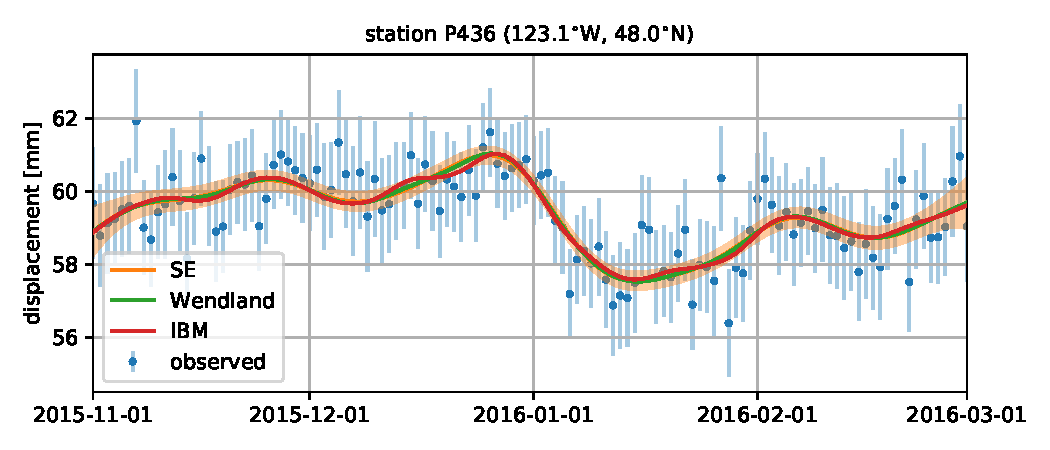
\includegraphics{ch5/figures/signal_fit/signal-fit.pdf}
\caption{Observed easting component of displacements at station P436 and predicted displacements when using different covariance functions for $T$. The one standard deviation uncertainties are shown for the observations and the predicted displacements when using the SE covariance function. For clarity, uncertainties are not shown for the IBM and Wendland covariance functions, but they are nearly equivalent to the uncertainties for the SE covariance function.}   
\label{ch5:fig:Fit}
\end{figure*}

\subsection{Transient strain rates}\label{ch5:sec:Results} 
Having established a noise model and a prior for transient displacements, we use the cleaned GNSS dataset to calculate transient strain rates in the Puget Sound region.  We calculate transient strain rates for each day from January 1, 2010 to May 15, 2017. The strain rates are estimates at a grid of points spanning the study area. In Figure \ref{ch5:fig:StrainMap} we show the transient strain rates on January 1, 2016, which coincides with the height of an SSE. We have included an animation showing the map view of strain rates through time as supplementary material. The strain rates shown in Figure \ref{ch5:fig:StrainMap} are generally similar to the strain rates during the other six SSEs considered in this study. The SSEs cause trench perpendicular compression in the Olympic Peninsula and extension east of Puget Sound. The strain transitions from compressional to extensional strain around the southern tip of Vancouver Island, which coincides with the location of where thrust slip tends to be inferred for SSEs in the Puget Sound region \citep[e.g.,][]{Dragert2001,Wech2009,Schmidt2010}. Thus, this pattern of strain is to be expected. During the period in between SSEs, secular strain rates indicate trench perpendicular compression throughout this study region \citep{Murray2000,McCaffrey2007,McCaffrey2013}. When comparing inferred strain rates from SSEs to the secular strain rates, we see that SSEs are concentrating tectonically accumulated strain energy towards the trench, and presumably pushing the subduction zone closer to failure. 

%A key difference between the strain inferred here and strain that can be derived from fault slip models is that our estimated strain rates are not based on an assumed physical model. In contrast, fault slip models can be biased by errors in the assumed fault geometry or lithospheric rheology. Moreover, the degrees of freedom in fault slip models usually cannot be constrained by GNSS data alone, and it is necessary to impose regularization which further biases the results. Since our estimated strain rates lack such systematic errors, we can be more confident that our solution is unbiased and has meaningful uncertainties.  

\begin{figure*}
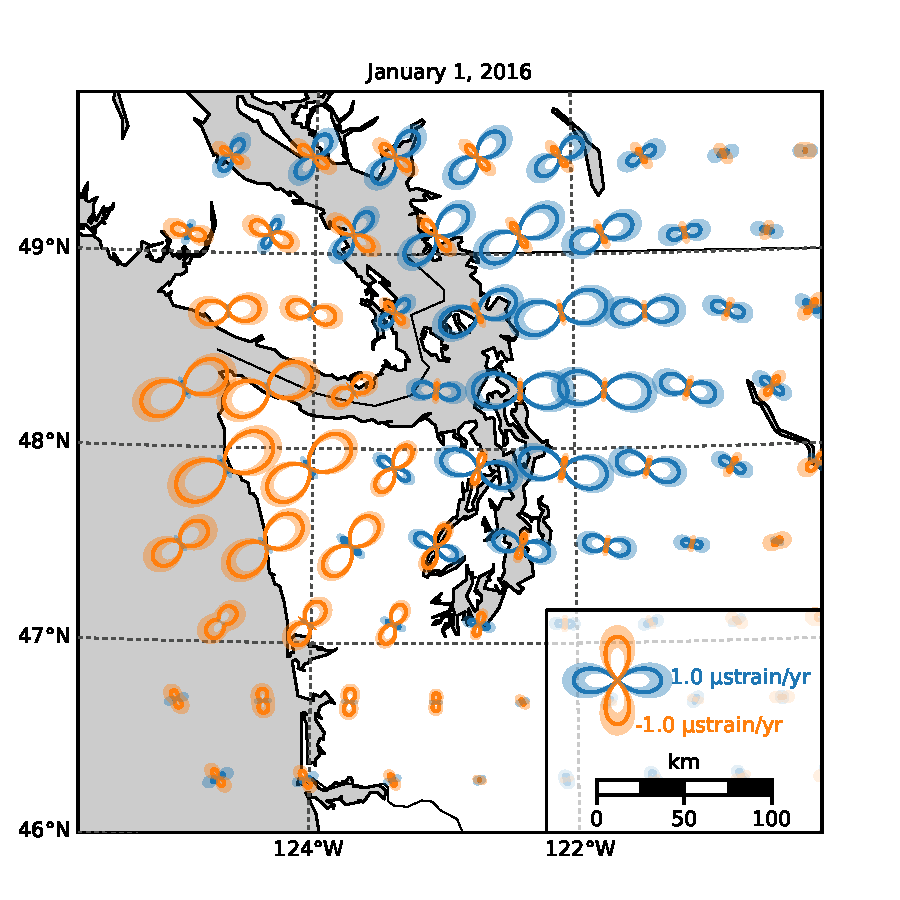
\includegraphics{ch5/figures/strain_map/strain-map.pdf}
\caption{Estimated transient strain rates during the Winter 2015-2016 SSE. Strain glyphs show the normal strain rate along each azimuth, where orange indicates compression and blue indicates extension. The shaded regions indicate one standard deviation uncertainties in the normal strain rates.}   
\label{ch5:fig:StrainMap}
\end{figure*}

In Figure \ref{ch5:fig:StrainTs} we show the time dependence of estimated transient strain rates at a position on the Olympic Peninsula, where transient strain rates from SSEs are largest. To verify that the estimated transient strain rates are accurately identifying geophysical signal, we compare the signal-to-noise ratio from eq. (\ref{ch5:eq:SNR}) to the frequency of seismic tremor (Figure \ref{ch5:fig:StrainMag}). A signal-to-noise ratio greater than ${\sim}3$ can be interpreted as a detected geophysical signal. For each detected event there is a corresponding peak in seismic tremor. We are also able to clearly identify transient strain associated with a more subtle SSE in August 2014. In between peaks in seismic tremor, the signal-to-noise ratio is consistently between 0 and 2, suggesting that all the transient strain detected at this location is associated with SSEs.

\begin{figure*}
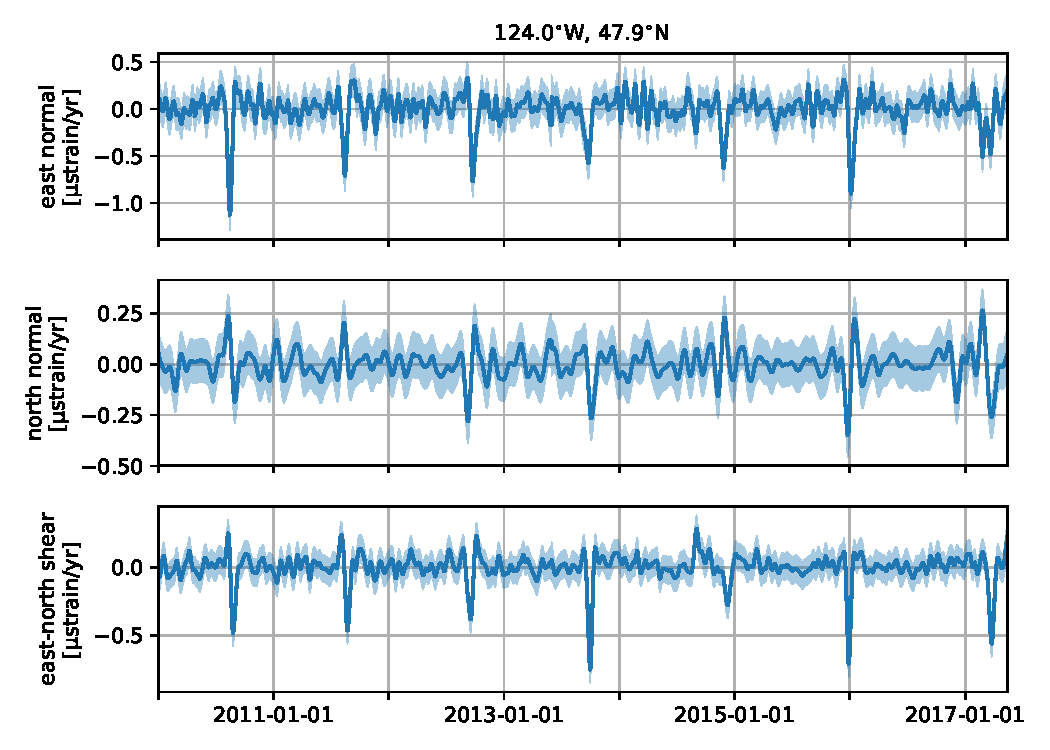
\includegraphics{ch5/figures/strain_ts/strain-ts.pdf}
\caption{Three components of the transient horizontal strain rate tensor estimated at the position shown in Figure \ref{ch5:fig:Context}. The shaded regions indicate one standard deviation uncertainty.}   
\label{ch5:fig:StrainTs}
\end{figure*}

\begin{figure*}
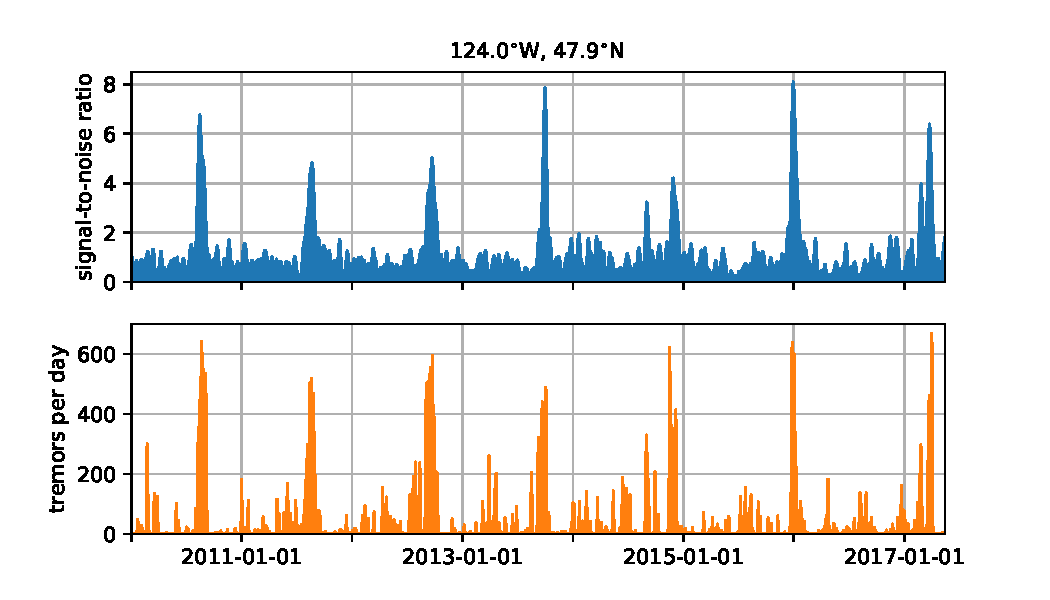
\includegraphics{ch5/figures/strain_ts/mag-ts.pdf}
\caption{(top) Signal-to-noise ratio (eq. \ref{ch5:eq:SNR}) at the position shown in Figure \ref{ch5:fig:Context}. (bottom) Frequency of tremors in the region shown in Figure \ref{ch5:fig:Context}.}   
\label{ch5:fig:StrainMag}
\end{figure*}

The results we have presented thus far indicate that we are identifying the strain that we should expect to see. There are, however, subtle features in our estimated transient strain rates which we were not expecting. For example, there is a brief period of east-west extension on the Olympic Peninsula several days prior to some of the SSEs. This feature can be seen before the summer 2012 and winter 2015-2016 SSEs in Figure \ref{ch5:fig:StrainTs} as well as in the supplementary animation. While this deformation is noteworthy, a discussion on the mechanisms causing it is outside the scope of this study.

\section{Discussion}\label{ch5:sec:Discussion}
Our results demonstrate that GPR is an effective tool for estimating transient strain from GNSS data, which can then be used to detect geophysical processes. One may argue that geophysical signal can also be detected by merely inspecting the GNSS displacement time series. Indeed, the SSEs identified in Figure \ref{ch5:fig:StrainMag} do produce visible displacements in the GNSS data. However, the GNSS data also contains outliers and non-tectonic deformation that is localized to individual stations. In contrast, our estimates of transient strain only identify features that are sufficiently spatially and temporally coherent, based on our chosen prior model. Furthermore, our estimates of transient strain are insensitive to common mode noise, which is highly spatially correlated noise resulting from factors such as reference frame error. Common mode noise can obscure geophysical signal in the GNSS data, but it gets canceled out when computing the transient strain. Lastly, our estimates of transient strain rates are a spatial and temporal derivative of displacements, and thus any geophysical signal in the transient strain rates tends to be more pronounced than in the GNSS data. For these reasons, we argue that transient strain rates estimated with the method described in Section \ref{ch5:sec:Method} can illuminate geophysical signal that may not be discernible from the noise in the GNSS displacement data. 

In addition to detecting geophysical processes, the GNSS derived transient strain rates can be used to better understand the data from borehole strain meters (BSMs). The Plate Boundary Observatory maintains about forty BSMs in the Pacific Northwest, and it has been demonstrated that BSMs are able to record transient geophysical events such as SSEs \citep[e.g.,][]{Dragert2011}. However, there are complications that prevent BSM data from being used quantitatively in geophysical studies. One difficulty is that BSM data should be calibrated with a well known strain source, such as diurnal and semidiurnal tides \citep{Hart1996,Roeloffs2010,Hodgkinson2013}. Unfortunately, the tidal forces at BSMs which record SSEs are strongly influenced by local bodies of water such as the Straight of Juan de Fuca, making it difficult to form a theoretical prediction of tidal strains \citep{Roeloffs2010}. Another complication is that noise in BSM data is not well understood. The noise consists, in part, of a long-term decay resulting from the instrument equilibrating with the surrounding rock \citep{Gladwin1987}. Typically, this noise is dealt with in an ad-hoc manner by fitting and removing exponentials and low-order polynomials. We envision that the GNSS derived strain rates from this paper can be used as a reference strain for calibrating BSM data and quantify its noise.    

There is potential for a more thorough analysis of the spatio-temporal noise in GNSS data, $\eta$, than what was performed in Section \ref{ch5:sec:NoiseModel}. We did not explore the spatial covariance of $\eta$, which would describe common mode noise. We are able to ignore common mode error in this study; however, for other geophysical studies based on GNSS data, such as fault slip inversions, it may be necessary to incorporate a spatially covarying noise model \citep[e.g.,][]{Miyazaki2003}. We can also improve upon the seasonal model used in this study, which consists of four spatially uncorrelated sinusoids for each station. We did not explore the spatial covariance of seasonal deformation or the temporal roughness (i.e., the number of sinusoids needed to describe the observations). The periodic Gaussian process \citep{Mackay1998} is an alternative model for seasonal deformation and is well suited for exploring the roughness of seasonal deformation.  The periodic Gaussian process has zero mean and the covariance function
\begin{equation}\label{ch5:eq:Periodic}
T(t,t') = \phi^2 \exp\left(\frac{-\sin(\pi|t - t'|)^2}{2\tau^2}\right).
\end{equation}
Realizations have annual periodicity and the roughness is controlled by $\tau$. Decreasing $\tau$ has the same effect as including higher frequency sinusoids in the seasonal model. The optimal value for $\tau$ can be found with the REML method as described in Section \ref{ch5:sec:NoiseModel}. 

The transient strain rates estimated in this study are constrained by about seven years of daily displacement observations from 94 GNSS stations. It can be computationally intensive to evaluate eqs. (\ref{ch5:eq:PosteriorMean3}) and (\ref{ch5:eq:PosteriorCov3}) for a dataset with this size. We significantly reduce the amount of memory needed to estimate transient strain rates by describing the temporal covariance of displacements with a compact Wendland covariance function. Using a compact covariance function for our prior turns eqs. (\ref{ch5:eq:PosteriorMean3}) and (\ref{ch5:eq:PosteriorCov3}) into sparse systems of equations, which we then solve with CHOLMOD. CHOLMOD is designed for solving sparse, positive definite systems of equations. The matrix being inverted in eqs. (\ref{ch5:eq:PosteriorMean3}) and (\ref{ch5:eq:PosteriorCov3}) is not positive definite; however, we can use another partitioned matrix inversion identity from \citet{Press2007} to partition it into positive definite submatrices to be inverted. Even when using a compact covariance function, it may still be necessary to reduce the computational burden by dividing the data into subsets and evaluating transient strain rates for each subset.   

\section{Conclusion}\label{ch5:sec:Conclusion}
In this paper we propose using Gaussian process regression (GPR) to estimate transient strain rates from GNSS data. Most other methods for estimating strain rates assume a parametric representation of deformation, which can bias the results if the parameterization is not chosen carefully. Here we assume a stochastic, rather than parametric, prior model for displacements. Our prior model describes how much we expect transient displacements to covary spatially and temporally. If we know nothing about the underlying signal that we are trying to recover, then the prior model can be chosen objectively with maximum likelihood methods. Because GPR is a Bayesian method, the uncertainties on our estimated transient strain rates are well quantified, allowing one to discern geophysical signal from noise. We demonstrate that GPR is an effective tool for detecting geophysical phenomena, such as slow slip events, in our application to GNSS data from Cascadia. One limitation with GPR is that it is not robust against outliers. To overcome this limitation, we have introduced an effective pre-processing method for identifying and removing outliers from GNSS datasets. Another complication with GPR is that it usually involves inverting a dense matrix where the number of rows and columns is equal to the number of observations. This is prohibitive when using several years of daily GNSS observations from a network of several hundred stations. We significantly reduce the computational burden of GPR by using compact Wendland covariance function to describe our prior model. While this paper just focuses on estimating transient strain rates, we believe that GPR is a powerful tool that can be applied to a wide range of geophysical problems.   

\section{Acknowledgements}
This material is based upon work supported by the National Science Foundation under grant EAR 1245263. The EarthScope Plate Boundary Observatory data is provided by UNAVCO through the GAGE Facility with support from the National Science Foundation (NSF) and National Aeronautics and Space Administration (NASA) under NSF Cooperative Agreement EAR-1261833. An implementation of the method described in this paper is named Python-based Geodetic Network Strain software (PyGeoNS). PyGeoNS is distributed under the MIT License and can be found at www.github.com/treverhines/PyGeoNS. 

\bibliographystyle{ch5/agu04}
\bibliography{ch5/refs5}  



\chapter{Validating Plate Boundary Observatory borehole
strainmeter data with GNSS derived strain}

\section{Introduction}
The Plate Boundary Observatory (PBO) contains 82 borehole strain
meters (BSMs), most of which are installed along the western United
States. BSMs are able to detect geophysical processes such as
coseismic and postseismic deformation
\citep[e.g.,][]{Langbein2006,Langbein2015}, slow slip events (SSEs)
\citep[e.g.,][]{Dragert2011}, and seismic wave propagation
\citep{Barbour2017}. BSMs are intended for measuring deformation over
timescales of minutes to months. At longer timescales, BSM data is
contaminated by factors such as borehole relaxation
\citep{Gladwin1987}. SSEs and postseismic deformation occur on
timescales that near the upper limit of what BSMs can be expected to
resolve. Another complication with BSM data is that the strain
measured at the borehole may deviate from the regional strain due to
local topographic or geologic features \citep{Berger1976}. Due to
these sources of noise, it can be difficult to use BSM data
quantitatively in, for example, geophysical inverse problems. In this
study, we assess the ability of BSMs to measure strain resulting from
SSEs on the Cascadia subduction zone. This is done by comparing BSM
data to strain derived from GNSS data.

\begin{figure}
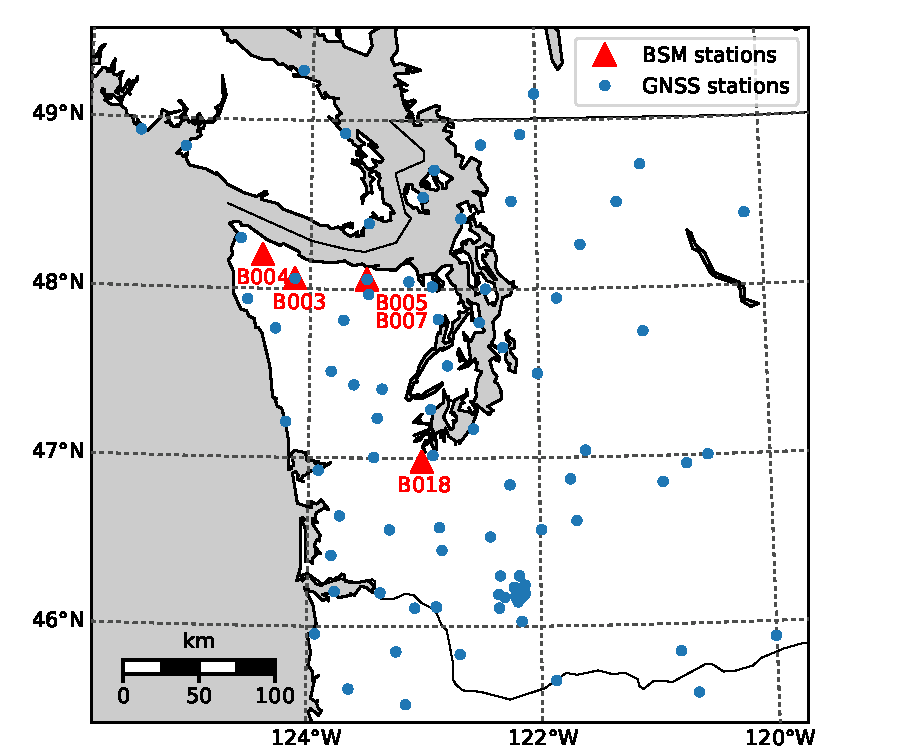
\includegraphics{ch6/figures/map.pdf}
\caption
[Location of BSM and GNSS stations used in this study]
{Location of BSM and GNSS stations used in this study.}   
\label{ch6:fig:Map}
\end{figure}

\section{BSM Data}
The are about forty PBO BSMs in the Pacific Northwest, and only five
of them, B003, B004, B005, B007, and B018, record noticeable
deformation from SSEs. We limit our attention to these five station in
this study.  The remaining stations either contain too much noise on
the timescale of SSEs or are too far away from the SSEs to observe any
strain. Each of the PBO BSMs are Gladwin four-component tensor
strainmeters, which are about 2 m long, 8.7 cm in diameter, and are
installed at about 100 to 200 m depth. Each BSM contains four
extensometers, or gauges. Only three gauges are necessary to
completely determine the horizontal strain tensor, and the fourth
gauge is included for redundancy. Gauges 1, 2, and 3 are oriented
$60^\circ$, $120^\circ$, and $150^\circ$ counterclockwise from gauge
0.

We use the level 2 gauge data provided by UNAVCO at www.unavco.org,
which has undergone several post-processing steps. In the level 2
gauge data a borehole curing trend is estimated and removed by fitting
two exponential terms and a linear trend to the data. The level 2 data
is corrected for tidal strains by estimating and removing sinusoids
with known tidal frequencies. There is also a correction for
barometric pressure because the normal stress imposed on the surface
by barometric pressure results in horizontal strains recorded by the
BSM. The barometric pressure correction is the observed barometric
pressure at each site multiplied by a best fitting scaling factor.
Lastly, offsets have been removed in the level 2 data product.

We denote the extension measured at gauge $i$ as $e_i$, and the
horizontal strain tensor components as $\varepsilon_{xx}$,
$\varepsilon_{yy}$, and $\varepsilon_{xy}$, where $x$ and $y$ indicate
the east and north direction, respectively. The extensions measured at
BSMs are traditionally converted to areal strain, $\varepsilon_a =
\varepsilon_{xx} + \varepsilon_{yy}$, differential strain,
$\varepsilon_d = \varepsilon_{xx} - \varepsilon_{yy}$, and engineering
shear strain, $\varepsilon_s = 2\varepsilon_{xy}$. We follow this
convention and use $\varepsilon_a$, $\varepsilon_d$, and
$\varepsilon_s$ for comparing BSM data to GNSS derived strains. Using
$\theta_0$ to denote the orientation of gauge 0, in degrees north of
east, these strain components can be expressed in terms of the gauge
measurements through the equation
\begin{equation}\label{ch6:eq:GaugeToStrain}
\left[\begin{array}{c}
\varepsilon_a \\
\varepsilon_d \\
\varepsilon_s \\
\end{array}\right]
=
2\mathbf{K}^{-1}\left[\begin{array}{ccc}
1 & \cos(2\theta_0) & \sin(2\theta_0) \\
1 & \cos(2(\theta_0 + 60)) & \sin(2(\theta_0 + 60)) \\
1 & \cos(2(\theta_0 + 120)) & \sin(2(\theta_0 + 120)) \\
1 & \cos(2(\theta_0 + 150)) & \sin(2(\theta_0 + 150)) \\
\end{array}\right]^+
\left[\begin{array}{c}
e_0 \\
e_1 \\
e_2 \\
e_3 \\
\end{array}\right],
\end{equation} 
where ``$+$" indicates the Moore-Penrose pseudoinverse and
$\mathbf{K}$ is a coupling matrix describing how the instrument
strains relate to the crustal strains \citep{Hart1996}. The components
$\varepsilon_a$, $\varepsilon_d$, and $\varepsilon_s$ represent
crustal strains, and $e_i$ are instrument strains. We assume that BSMs
are installed in homogeneous, isotropic rock, allowing us to write the
coupling matrix as
\begin{equation}\label{ch6:eq:CouplingMatrix}
\mathbf{K} = 
\left[\begin{array}{ccc}
c & 0 & 0 \\
0 & d & 0 \\
0 & 0 & d \\
\end{array}\right],
\end{equation}  
where $c$, and $d$ are response factors that depend on the elastic
properties of the instrument, the grout, and surrounding rock
\citep{Gladwin1985}. Based on the analysis of \citet{Gladwin1985}, we
use $c=1.5$ and $d=3.0$. UNAVCO, the organization responsible for
maintaining the PBO BSMs and disseminating their data, use these same
response factors for their final data products.

Local topographic or geologic features can cause $\mathbf{K}$ to have
non-zero off diagonal elements. If possible, the components of
$\mathbf{K}$ should be determined in-situ by calibrating the BSM data
with a well known strain source, such as diurnal and semi-diurnal
tides \citep{Hart1996,Roeloffs2010,Hodgkinson2013}. \citet{Hart1996}
calibrated a BSM at Pinyon Flat, using the tidal strains recorded at a
collocated laser strain meter. This calibration method is, of course,
not possible for most PBO BSMs. \citet{Roeloffs2010} and
\citet{Hodgkinson2013} calibrated PBO BSMs using theoretical
predictions of tidal strains \citep[e.g.,][]{Agnew1997}. This approach
is still not adequate for BSMs near large local bodies of water, which
can make it difficult to form an accurate theoretical estimate of
tidal strains. As determined by \citet{Roeloffs2010}, the five BSM
stations considered in this paper are too close to the Straight of
Juan de Fuca to be accurately calibrated with tidal strains. Since
in-situ calibration is not possible, we note that our choice for
$\mathbf{K}$ is likely to be a significant source of error in BSM
data. Another potential source of error is the assumed orientation for
$\theta_0$. This orientation is determined by a compass on the
instrument, and it is possible that magnetic minerals in the
surrounding rock can give the compass an incorrect reading.

\section{GNSS derived strain}
We compare the BSM strain components to transient strains estimated
from GNSS data. Here we consider transient strains to be any deviation
from the secular strain rate.  We use daily GNSS displacement
solutions for 94 continuous GNSS stations in the Pacific Northwest
(Figure \ref{ch6:fig:Map}). This data has also been made available through
UNAVCO. We convert the GNSS data to transient strains using Gaussian
process regression (GPR) as described in \citet{Hines2017a}. With GPR,
we select a prior spatio-temporal covariance model for the geophysical
signal that we want to recover. Following \citet{Hines2017a}, we
assume that our prior for displacements is a Gaussian process with
zero mean, and covariance function described by
\begin{equation}\label{cov}
C_u((t,x),(t',x')) = \phi^2 T(t,t')X(x,x'),
\end{equation}        
where $T$ is the Wendland covariance function
\begin{equation}\label{ch6:eq:Wendland}
T(t,t') = \left(1 - \frac{|t - t'|}{\tau}\right)^5_+ \left(\frac{8|t - t'|^2}{\tau^2} + \frac{5|t - t'|}{\tau} + 1\right), 
\end{equation}
and $X$ is the squared exponential covariance function
\begin{equation}\label{ch6:eq:SE}
X(\vec{x},\vec{x}') = \exp\left(\frac{-||\vec{x} - \vec{x}'||_2^2}{2 \ell^2}\right).
\end{equation}
The hyperparameters $\phi$, $\tau$, and $\ell$ control the amplitude,
characteristic time-scale, and characteristic length-scale of the
prior, respectively. \citet{Hines2017a} found that the optimal
hyperparameters for describing displacements from SSEs are roughly
$\phi =$ 0.5 mm, $\tau =$ 0.1 yr, and $\ell =$ 100 km. These
parameters were chosen objectively using maximum likelihood methods;
however based on our experience, this prior may not be sufficiently
flexible to described all the observed data. Consequently, we explore
using lower values for $\tau$ and $\ell$ and a higher value for
$\phi$. For each tested set of hyperparameters, we condition the prior
with the observed GNSS data and visually compare the posterior
displacements to the observations. We settle on the values $\phi =
1.0$ mm, $\tau =$ 0.05 yr, and $\ell =$ 80 km. With this final set of
hyperparameters, we condition the prior with the GNSS data and then
spatially differentiate the posterior displacements to obtain
transient strain.

\begin{figure}
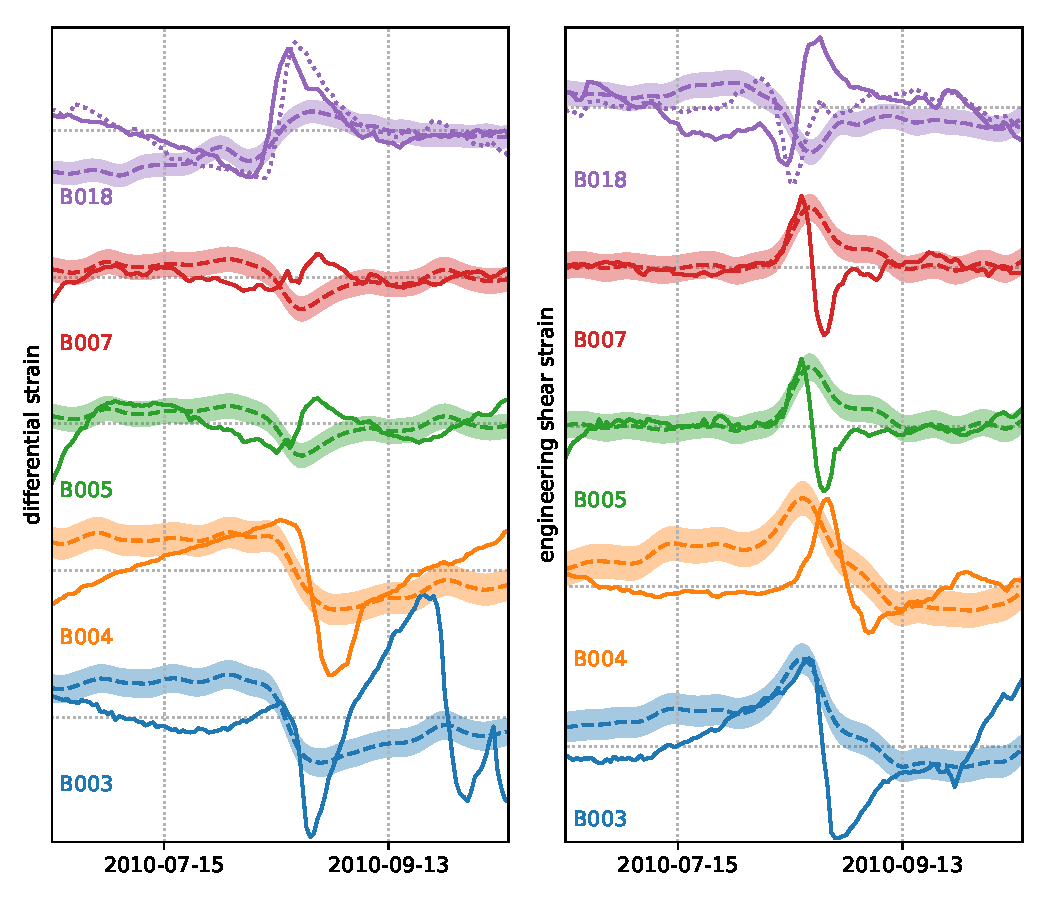
\includegraphics{ch6/figures/SSE1.pdf}
\caption
[BSM and GNSS derived strains for the summer 2010 SSE]
{differential (left) and engineering shear (right) strains
during the summer 2010 SSE observed at BSMs (solid) and derived from
GNSS data (dashed). The horizontal dotted lines are spaced by 0.1
micro-strain. The shaded region around the GNSS derived strains show
the one standard deviation confidence interval. The dotted line for
station B018 shows the BSM data using the optimal instrument
orientation. The shown BSM data has been detrended by estimating and
removing a second-order polynomial from each timeseries.}
\label{ch6:fig:SSE1}
\end{figure}

\section{Results}
We compare the BSM data to GNSS derived strains for eight SSEs in the
Puget Sound region. The earliest SSE considered occurred in spring
2009 and the latest SSE occurred in winter 2017. The two datasets are
in best agreement for the summer 2010 SSE, which is shown in Figure
\ref{ch6:fig:SSE1}. The data for the remaining SSEs are included at the
end of this manuscript in Figures \ref{ch6:fig:SSE0} through
\ref{ch6:fig:SSE7}. We only show the differential and engineering shear
strains because there is no clear signal in the areal strain for
either the GNSS derived strains or the BSM data. \citet{Roeloffs2010}
also expressed doubt in the areal strains measured at stations B003,
B004, B007, and B018 because the areal strains derived from different
combinations of gauges at these stations are not self consistent.
\citet{Roeloffs2010} also noted an inconsistency in the differential
strains at B003.

Station B004 records differential and engineering shear strains that
are most consistent with the GNSS derived strains. However, the
initiation of SSE strains recorded at B004 tend to lag several days
behind the GNSS derived strains. The strain rates recorded at B004
also tend to be greater than the GNSS derived strains. One possible
explanation for this discrepancy is that the GNSS station spacing is
too wide to resolve a relatively sharp pulse of strain from the SSE as
it traverses along the subduction zone.

The engineering shear strain, but not the differential strain,
recorded at B003 contain a clear signal from each SSE that is
consistent with the GNSS derived strains. Similar to B004, the
recorded strain rates exceed those predicted by the GNSS data. There
are many spurious features in the differential strains recorded at
B003, which makes it difficult determine whether or not that component
contains signal from SSEs.

Stations B005 and B007, which are located within a few hundred meters
of each other, both show clear SSE signals in their engineering shear
strains.  However, the temporal pattern of strain recorded at these
stations are not consistent with the GNSS derived strains.  For the
summer 2010 and summer 2011 SSEs, the GNSS derived strains predict a
single positive pulse of engineering shear strain at these locations,
but both B005 and B007 record an initially positive pulse that then
becomes negative. We cannot explain this discrepancy with mis-oriented
instruments because both B005 and B007 would need to have nearly
identical orientation errors. If the negative pulse of engineering
shear strain were a regional ($\gtrsim$50 km scale) feature, then it
would have been recognized in the GNSS data. We then suspect that the
discrepancy can be explained with topographic of geologic features
that may distort the local strain field. While, we are not saying that
the engineering shear strains at B005 and B007 are erroneous, it is
clear that they are inconsistent with the regional scale strains. The
differential strains at station B005 and B007 do not show any clear
SSE signal, even though a signal is observed in the GNSS derived
strains. This too could be due to distortion of the strain field from
local features.

\begin{figure}
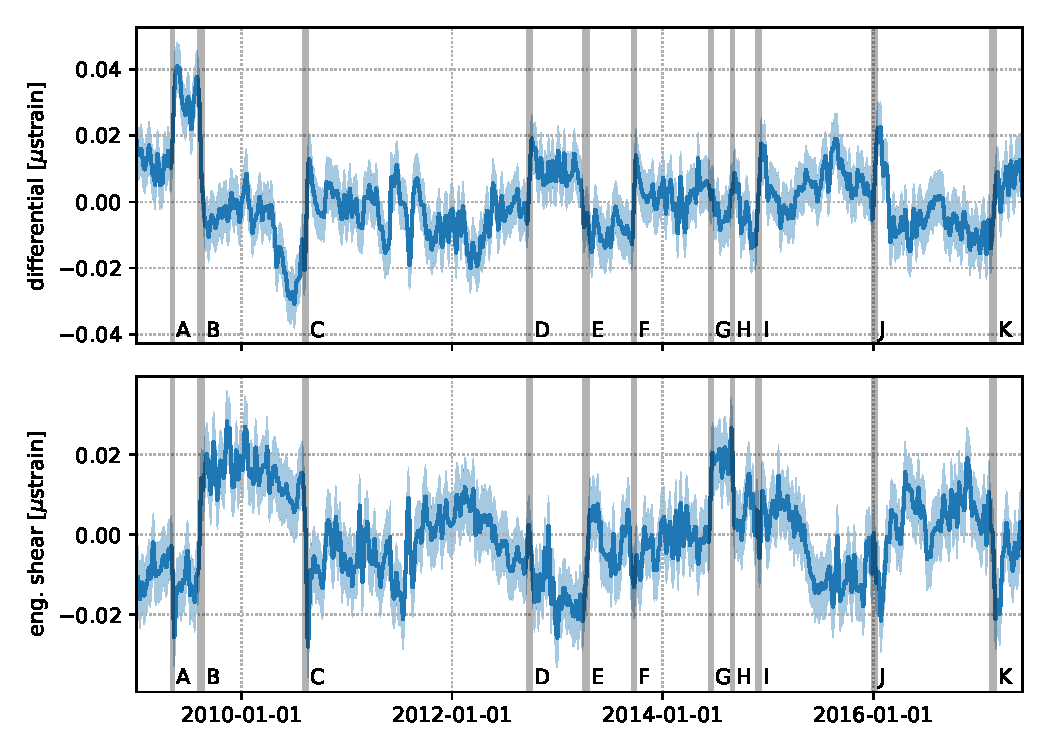
\includegraphics{ch6/figures/gnss.pdf}
\caption
[GNSS derived strains for station B018]
{GNSS derived differential and engineering shear strains for
station B018. The shaded blue regions indicate the one standard
deviation confidence interval. The shaded gray regions indicate times
of strain drops, which are the result of SSEs.}
\label{ch6:fig:Gnss}
\end{figure}

\begin{figure}
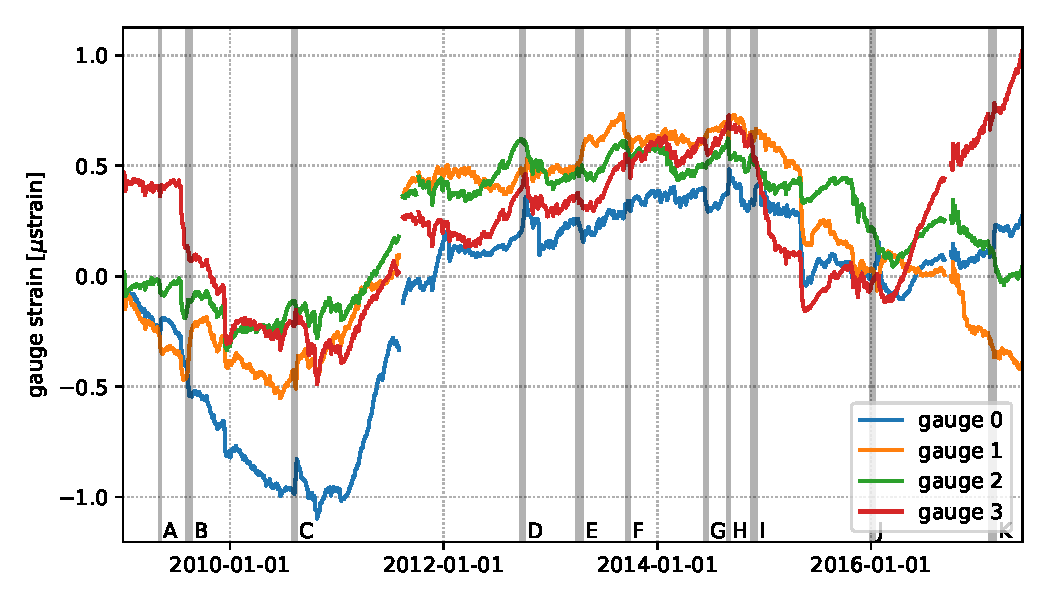
\includegraphics{ch6/figures/gauge.pdf}
\caption
[Gauge readings at station B018]
{Gauge readings at station B018. The gray shaded regions
indicate times of strain drops from Figure \ref{ch6:fig:Gnss}.}
\label{ch6:fig:Gauge}
\end{figure}

\begin{figure}
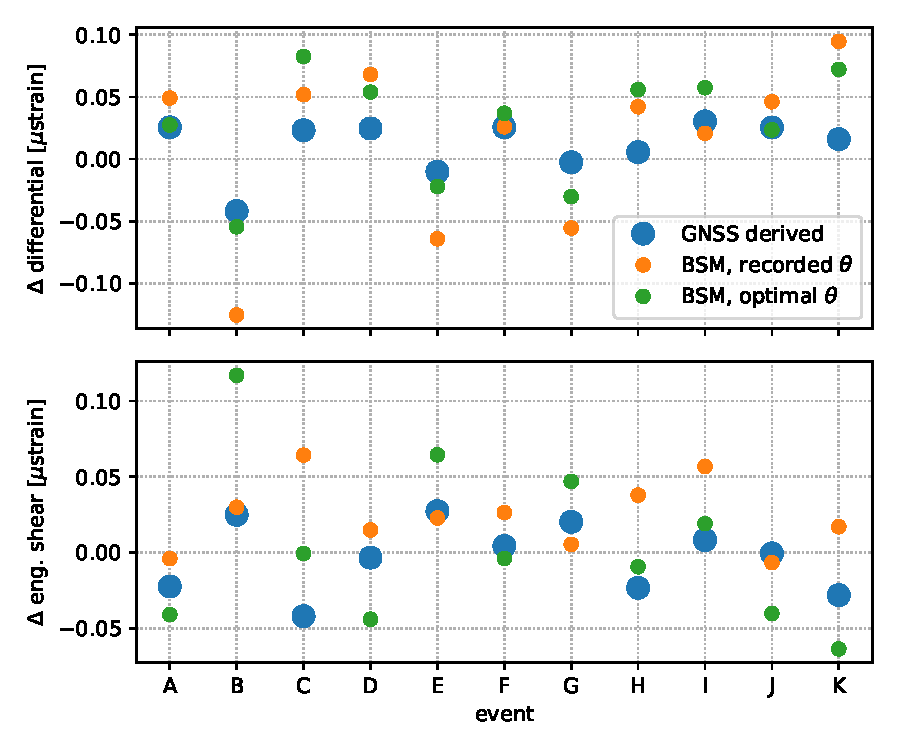
\includegraphics{ch6/figures/fit.pdf}
\caption
[GNSS and BSM strain dropts at station B018]
{GNSS derived strain drops at station B018 during the 11
events identified in Figure \ref{ch6:fig:Gnss} (blue dots), BSM strain
drops using the recorded orientation for B018 (orange dots), and BSM
strain drops using the optimal orientation for B018 (green dots).}
\label{ch6:fig:Fit}
\end{figure}

\begin{figure}
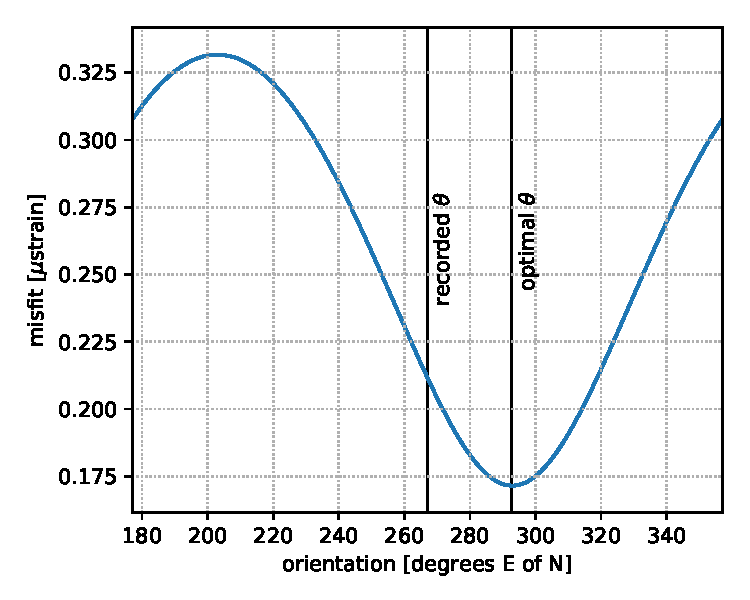
\includegraphics{ch6/figures/misfit.pdf}
\caption
[Misfit as a function of instrument orientation for station
B018]
{Misfit as a function of instrument orientation for station
B018.}
\label{ch6:fig:Misfit}
\end{figure}

The differential and engineering shear strains recorded at station
B018 have notably less noise than most BSMs. Nonetheless, the
engineering shear strains at B018 are not consistent with the GNSS
derived strains. For example, BSM data shows a strain increase from
the summer 2010 SSE, and the GNSS derived strains predict a strain
decrease with about equal magnitude. We consider the possibility that
this discrepancy is due to an error in the instrument orientation, and
we identify a new, optimal orientation for station B018. We want to
find the value for $\theta_0$ that causes the strain drops (or
increases) recorded at B018 to best match the strain drops derived
from GNSS data. We identify 11 strain drops in the GNSS derived
strains, which are due to SSEs in the Puget Sound region and in Oregon
(Figure \ref{ch6:fig:Gnss}). We define strain drops as the total strain
change over the hand-selected intervals shown in Figure
\ref{ch6:fig:Gnss}. The strain drops for each event are shown in Figure
\ref{ch6:fig:Fit}. For each tested $\theta_0$, we use eq.
(\ref{ch6:eq:GaugeToStrain}) to convert the strain drops recorded at each
gauge (Figure \ref{ch6:fig:Gauge}) to the differential and engineering
shear strain drops. We then use the L2 norm of the residuals, the
difference between the BSM strain drops and the GNSS derived strain
drops, as the misfit metric. We find an optimal value of $\theta_0$ to
be $293^\circ$ east of north, which can be compared to the recorded
value of $267^\circ$ (Figure \ref{ch6:fig:Misfit}). With the new
orientation, the engineering shear strain recorded at B018 decreases
during the summer 2010 SSE, which is now consistent with the GNSS data
(Figure \ref{ch6:fig:SSE1}). The differential strains at B018 are roughly
consistent with the GNSS derived strains, regardless of whether the
recorded $\theta_0$ or optimal $\theta_0$ is used.

\section{Conclusion}
We have compared BSM data to GNSS derived strains for eight of the
past SSEs in the Puget Sound region. The summer 2010 SSE produced the
clearest signal in both the BSM data and GNSS derived strain, and yet
it is still difficult to reconcile the two datasets. Of the five BSM
stations that record strain from SSEs, only one of them, B004, records
differential and engineering shear strains that are consistently in
agreement with the GNSS derived strains. For station B003, only the
engineering shear strains are consistent with the GNSS data. Both the
differential and engineering shear strains recorded at B018 can be
made to agree with the GNSS data when assuming a new instrument
orientation. For station B005 and B007 it may be necessary to use a
coupling matrix other than the isotropic one considered in this study.
We are unaware of a reliable calibration method for these stations,
since tidal calibration is not possible. In general, we urge caution
when attempting to use BSM data to describe regional strains.

\begin{figure}
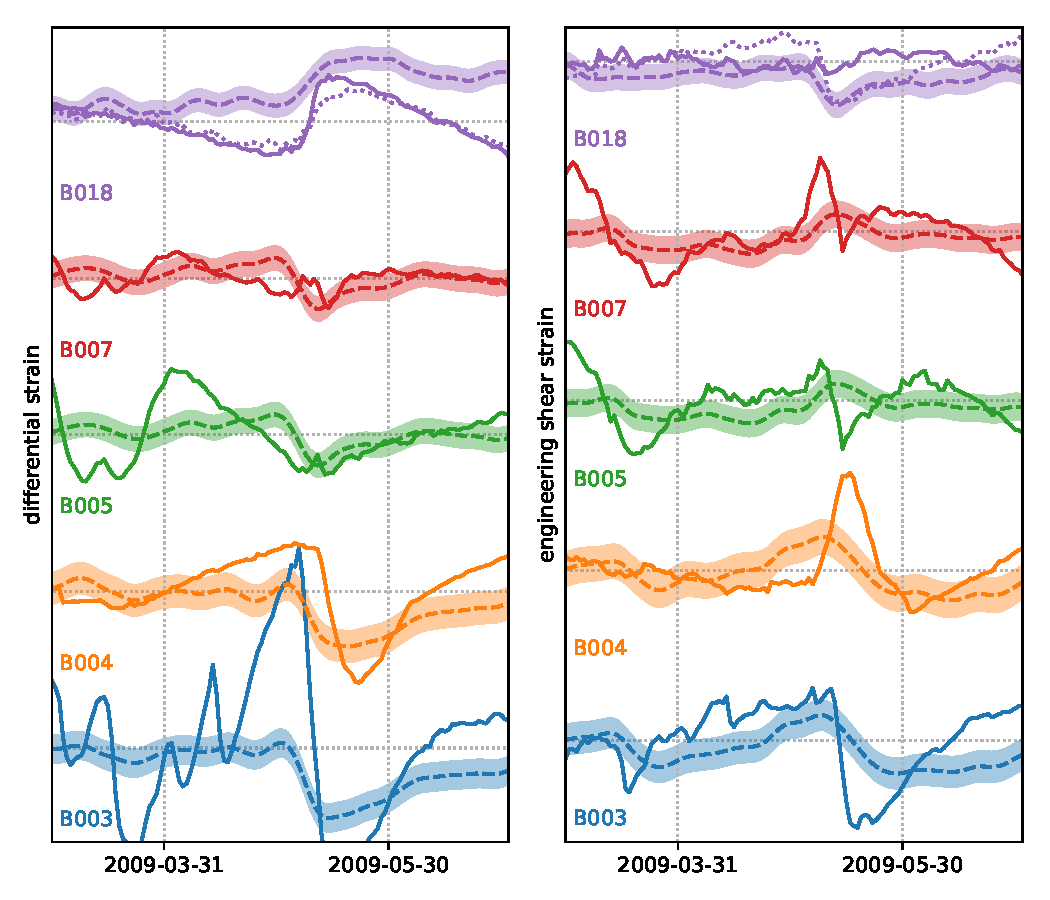
\includegraphics{ch6/figures/SSE0.pdf}
\caption
[BSM and GNSS derived strains for the spring 2009 SSE]
{Same as Figure \ref{ch6:fig:SSE1}, but for the spring 2009 SSE.}   
\label{ch6:fig:SSE0}
\end{figure}

\begin{figure}
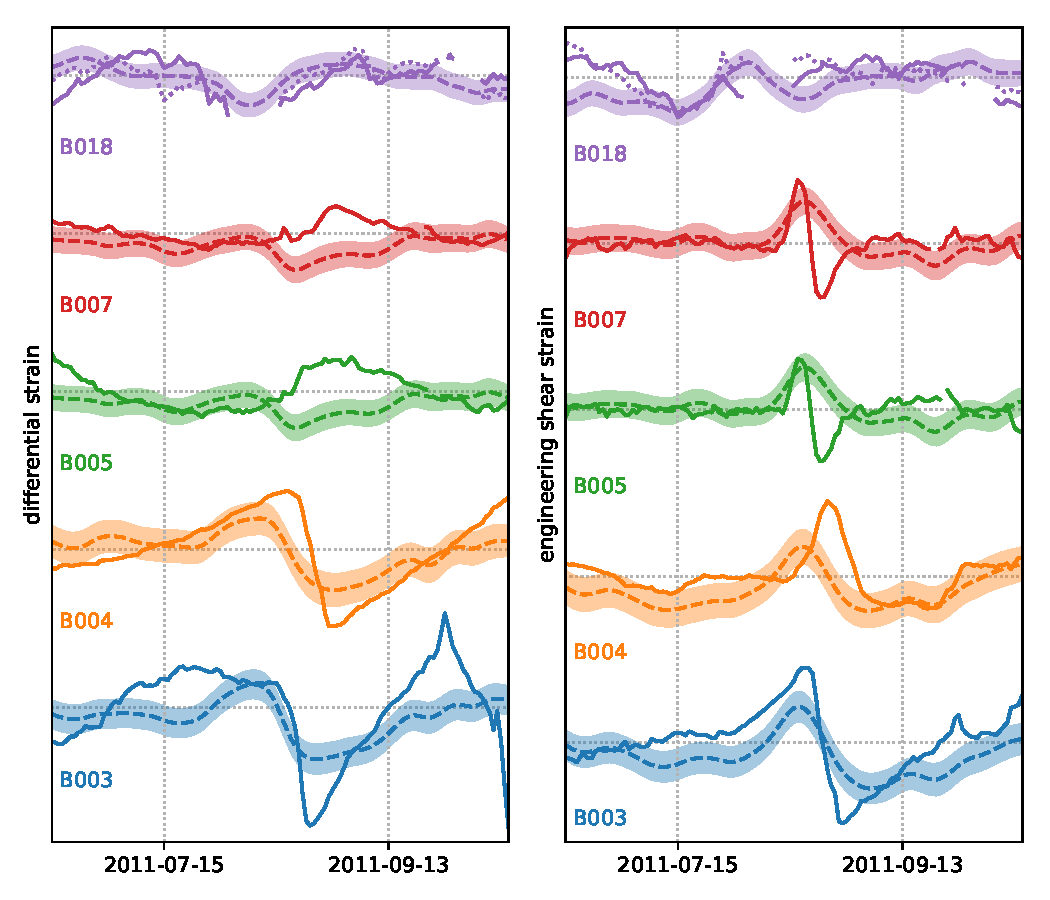
\includegraphics{ch6/figures/SSE2.pdf}
\caption
[BSM and GNSS derived strains for the summer 2011 SSE]
{Same as Figure \ref{ch6:fig:SSE1}, but for the summer 2011 SSE.}   
\label{ch6:fig:SSE2}
\end{figure}

\begin{figure}
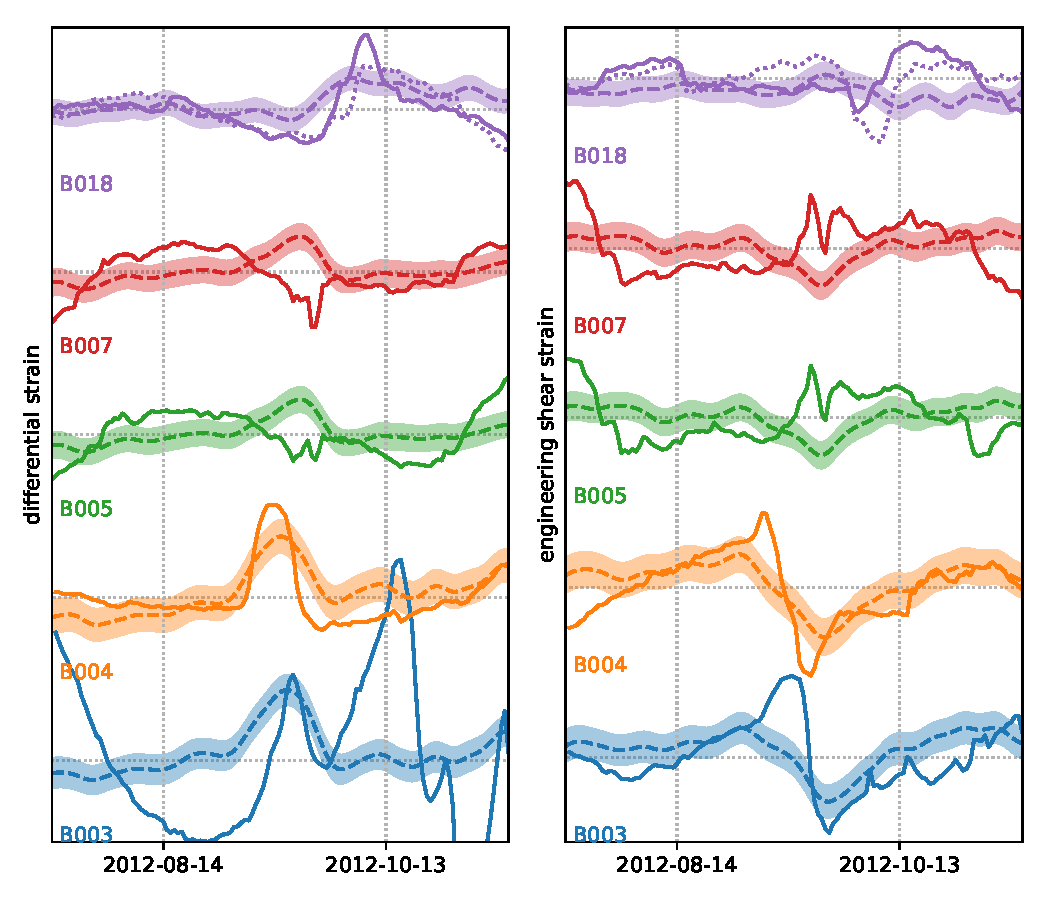
\includegraphics{ch6/figures/SSE3.pdf}
\caption
[BSM and GNSS derived strains for the summer 2012 SSE]
{Same as Figure \ref{ch6:fig:SSE1}, but for the summer 2012 SSE.}   
\label{ch6:fig:SSE3}
\end{figure}

\begin{figure}
\includegraphics{ch6/figures/SSE4.pdf}
\caption
[BSM and GNSS derived strains for the fall 2013 SSE]
{Same as Figure \ref{ch6:fig:SSE1}, but for the fall 2013 SSE.}   
\label{ch6:fig:SSE4}
\end{figure}

\begin{figure}
\includegraphics{ch6/figures/SSE5.pdf}
\caption
[BSM and GNSS derived strains for the fall 2014 SSE]
{Same as Figure \ref{ch6:fig:SSE1}, but for the fall 2014 SSE.}   
\label{ch6:fig:SSE5}
\end{figure}

\begin{figure}
\includegraphics{ch6/figures/SSE6.pdf}
\caption
[BSM and GNSS derived strains for the winter 2015-2016 SSE]
{Same as Figure \ref{ch6:fig:SSE1}, but for the winter 2015-2016 SSE.}   
\label{ch6:fig:SSE6}
\end{figure}

\begin{figure}
\includegraphics{ch6/figures/SSE7.pdf}
\caption
[BSM and GNSS derived strains for the winter 2017 SSE]
{Same as Figure \ref{ch6:fig:SSE1}, but for the winter 2017 SSE.}   
\label{ch6:fig:SSE7}
\end{figure}

%\bibliographystyle{agu04}
%\bibliography{refs}  


\bibliographystyle{agu04}
\bibliography{refs}

\end{document}
